%\documentclass[MSc, titlepagenumber=off]{icldt}

\documentclass[a4paper,11pt,twoside]{report}
\usepackage[left=2.5cm,right=2cm,top=2cm,bottom=2cm]{geometry}

\usepackage{graphicx}
\usepackage[T1]{fontenc}
\usepackage[scaled]{beramono}
\usepackage{amssymb}
\usepackage{amsmath}
\usepackage[lofdepth,lotdepth]{subfig}
\usepackage{paralist}
\usepackage{stfloats}
\usepackage[table]{xcolor}
\definecolor{lightgray}{gray}{0.9}
\newcommand{\classname}[1]{\texttt{#1}}

\usepackage{enumitem}
\usepackage{float}
\usepackage{url}

\usepackage{color}
\definecolor{bluekeywords}{rgb}{0.13,0.13,1}
\definecolor{greencomments}{rgb}{0,0.5,0}
\definecolor{redstrings}{rgb}{0.9,0,0}

\usepackage{algorithm}
\usepackage{algorithmic}

\usepackage{listings}
\usepackage[toc,page]{appendix}

\DeclareCaptionFont{white}{\color{white}}
\DeclareCaptionFormat{listing}{\colorbox{gray}{\parbox{\textwidth}{#1#2#3}}}
\captionsetup[lstlisting]{format=listing,labelfont=white,textfont=white}
\definecolor{javared}{rgb}{0.6,0,0} % for strings

\definecolor{javagreen}{rgb}{0.25,0.5,0.35} % comments

\definecolor{javapurple}{rgb}{0.5,0,0.35} % keywords

\definecolor{javadocblue}{rgb}{0.25,0.35,0.75} % javadoc
%make sure coding for all implementation paragraphs is relevant and up to date
\lstset{language=Java,
keywordstyle=\color{javapurple}\bfseries,
stringstyle=\color{javared},
commentstyle=\color{javagreen},
morecomment=[s][\color{javadocblue}]{/**}{*/},
basicstyle=\small\ttfamily,
numbers=none,
numberstyle=\tiny\color{gray},
columns=fullflexible,
frame=none,
showstringspaces=false
stepnumber=2,
numbersep=10pt,
tabsize=4,
showspaces=false,
breaklines = true,
breakautoindent=true,
breakatwhitespace = true
}

\newcommand{\blankpage}{
\newpage
\thispagestyle{empty}
\mbox{}
\newpage
}

%%Change caption name in code snippets
%\renewcommand*{\lstlistingname}{Code}

%\title{Sampling in a Large Network\\Final Report}
%\author{Xenofon Foukas}
%\date{}
% Please specify you department here.
%\department{Computing}
% The college regulations do not require that you mention 
% your supervisor on the titlepage of you dissertation.
% If you want to do so put her name here.
%\supervisor{\textit{Professor Alexander Wolf}}
% The college regulations do neither require nor forbid 
% a dedication of your dissertation to somebody or something. 
% If you want to include a dedication put the text here. 
%\dedication{}
%\college{Imperial College London}
%\field{Advanced Computing}


%\setlength{\topmargin}{0in}
%\setlength{\headheight}{0in}
%\setlength{\headsep}{0in}

%\setlength{\textwidth}{6.5in}
%\setlength{\oddsidemargin}{-0.12in}
%\setlength{\evensidemargin}{-0.12in}

\setdescription{leftmargin=\parindent,labelindent=\parindent}
\begin{document}


%\maketitle
  \begin{titlepage}

 

 \par

  \clearpage

  \thispagestyle{empty}

  

 \noindent\begin{minipage}[t]{\textwidth}

   \centering\large

   Imperial College London\\

   Department of Computing

  \end{minipage}

 

 

 \vskip 15em

 

 \begin{center}

   {\huge \textbf{Sampling in a Large Network} \par}

   \vskip 3em

   {\Large \lineskip 0.75em

   \begin{tabular}[t]{c}

    by\\\\

    Xenofon Foukas

   \end{tabular}\par}

   \vskip 1.5em

  \end{center}\par

 

 \vskip 24em

 \noindent\begin{minipage}[b]{\textwidth}

   \centering 

   Submitted in partial fulfilment of the requirements for the degree of\\

   Master of Science in Advanced Computing of Imperial College London

  \end{minipage}

 \vskip 5em

 \noindent\begin{minipage}[b]{\textwidth}

   \centering 

   September 2013

  \end{minipage}

 

 

 \end{titlepage}

\blankpage

\begin{abstract}


Decentralized networks are a very popular architectural design, since they are usually characterized by reliability and resiliency to failures, while offering high performance with a relatively small infrastructure cost. However, one of the disadvantages of such networks is the difficulty of computing some global properties, which are required, even as approximations, in numerous tasks, such as searching and maintenance. Computing these properties using either centralized or decentralized algorithms is generally a feasible task. However, the real challenge is finding a solution that can be efficient both in terms of time and communication cost.

In this project we propose a fully decentralized protocol implementing the Impulse response algorithm by Carzaniga et al. \cite{6195806}. This algorithm uses impulse measurements from neighboring nodes for the estimation of the network's spectrum, which can be used for deriving useful network properties like the mixing time. We propose an extension of the original approach to make our protocol robust in the presence of churn (unstable networks) by executing multiple partially overlapping instances of the impulse algorithm. We follow a layered approach which offers our protocol portability allowing its deployment into various networks with little effort from the developer. Finally, we present a realistic scenario of usage for this protocol in the form of a simple application for estimating the average number of files stored in any network node.


\end{abstract}

\blankpage

\thispagestyle{empty}
\section*{Acknowledgments}

I would like to thank my supervisor, Professor Alexander Wolf, for believing in me and giving me the opportunity to work on this project, as it turned out to be a very exciting and rewarding experience.  His comments and suggestions were very helpful and shaped a large part of my work.

I would also like to thank Professor Antonio Carzaniga from the University of Lugano for giving me some very useful advice regarding some technical issues, which greatly improved my final results.

A special thanks goes to my family, not only for their financial support throughout this year, but mostly for always being there for me, supporting me even from a distance.

Finally, I would like to thank all my friends for being so supportive and cheering me up whenever I was in a bad mood or felt disappointed.


\blankpage

\tableofcontents
\listoffigures
\listoftables
\blankpage




\chapter{Introduction}

\section{Motivation}


It is very often beneficial to architect networks and overlays as fully decentralized systems rather than choosing a centralized architectural design. Such an approach usually leads to networks that are more reliable and resilient to failures, while offering high performance with a relatively small infrastructure cost. Moreover, since only local information are being used for making decisions, no component has a complete view or control over the whole network, resulting in a more flexible and secure model. For instance, common network activities such as packet routing no longer rely in a single node for control and coordination, which could turn out to be a bottleneck or a single point of failure. A very popular example of a decentralized architecture are peer-to-peer (P2P) networks, in which individual nodes communicate with each other sharing their resources (e.g. processing power, memory etc) both as suppliers and as consumers. A wide range of services are based on protocols that run on peer-to-peer networks, which are often comprised of thousands or millions of nodes (e.g. BitTorrent).

\begin{figure}[h]
\centering
\subfloat[][A centralized network]{
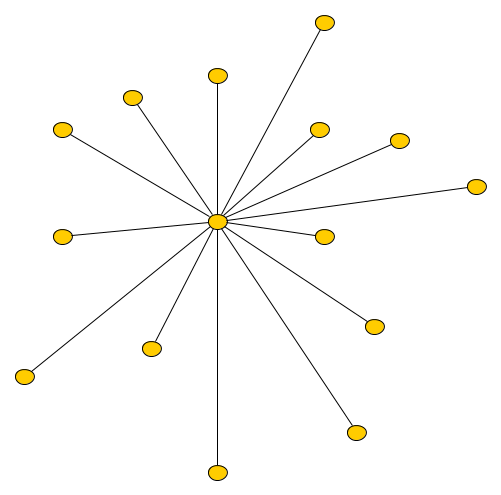
\includegraphics[width=0.3\textwidth]{../figures/centralized.png}
\label{fig:centralized}}
\qquad
\subfloat[][A decentralized network]{
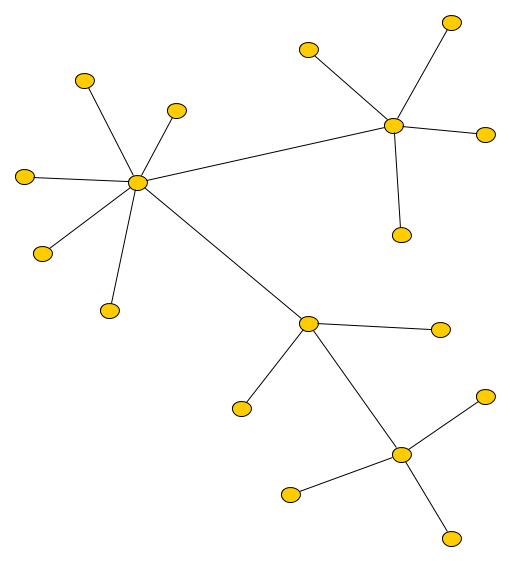
\includegraphics[width=0.3\textwidth]{../figures/decentralized.png}
\label{fig:decentralized}}
\caption{Centralized vs Decentralized networks}
\end{figure}

Regardless of the benefits that a decentralized architecture offers, it is very often necessary to compute global properties of the network which are required, even as approximations, in numerous tasks, such as searching and maintenance. Some typical examples of common global properties are the size of the network and its mixing time, i.e. the number of hops after which a random walk approaches the network's stationary distribution and becomes independent of the starting point. Computing these properties using either centralized or decentralized algorithms is generally a feasible task. However, the real challenge is finding a solution that can be efficient both in terms of time and communication cost.\\


There exist many proposals for efficient computation of global parameters in decentralized systems, each following different approaches, from sampling and projecting local properties to computing aggregates of data distributed over the network. Some algorithms are based on deriving useful properties from the spectrum of the network by computing the most significant eigenvalues of some descriptive matrix. There has been a proposal of a particularly interesting fully decentralized algorithm by Carzaniga et. al\cite{6195806} that can compute efficiently some global properties like the mixing time, by using the eigenvalues of a matrix closely related to the adjacency matrix of the network. While this algorithm appears to have good results in a simulation environment it has not been tested using some concrete implementation. Additionally, the estimates it provides are lacking accuracy in networks with high churn rates. Thus, it would be interesting to better investigate the algorithm's potential and to try and improve its weaknesses.


\section{Contributions}

In this project we try to design and implement a protocol based on the decentralized estimation algorithm proposed by Carzaniga et al. \cite{6195806}. Such a protocol should be able to efficiently perform the tasks required by the algorithm, while it should be designed in a way that allows its deployment into common network and overlay topologies, e.g. a Chord or Pastry topology. In addition, the project should attempt to enhance the proposed algorithm's robustness for better estimations in networks with high churn rates. This enhancement is important, since it will allow the algorithm to be applied in more realistic networks. For instance most common peer-to-peer networks are by nature unstable, since nodes continuously join and depart from the network, altering its topology and consequently its properties.\\

This project presents both theoretical and practical issues that need to be addressed in an elegant and efficient way. The nature of the project presents us with two main challenges. The first challenge is to design a protocol that is robust and efficient while remaining simple and to implement it with extensibility in mind, both in functionality and in compliance with a variety of underlying network communication protocols. The second challenge is that such a protocol should be evaluated in an environment that closely resembles a real large-scale network. This will allow us to better determine its applicability and usefulness in real-life scenarios. 


\section{Report Structure}

We begin by making a short introduction on decentralized networks, presenting techniques and related work in computing global properties of networks and overlays in Chapter \ref{sec:background}. We also make a short introduction into dynamic systems and realization algorithms, which will allow us to present and explain in greater depth the decentralized algorithm that will form the basis of our proposed protocol, discussing both its evaluation results and limitations.\\

In Chapter \ref{sec:design} we present the design requirements that our proposed protocol should fulfill, discussing both advantages and disadvantages that certain design decisions might incur to the applicability and efficiency of our proposal. Moreover, the general design overview of the proposed protocol is discussed and its constituent components are presented. The actual implementation of the protocol is presented in chapter \ref{sec:implementation}, where technical details are analyzed and justified in depth, also presenting optimizations performed and possible alternative solutions that were considered.\\

Chapter \ref{sec:evaluation} evaluates the success of this project and limitations and presents a realistic scenario of usage for this protocol in the form of a simple application for estimating the average number of files stored in any network node. Finally, Chapter \ref{sec:conclusion} presents a summary of the project and discusses possible future work.


\chapter{Background}
\label{sec:background}

This chapter makes a short introduction on networking concepts and technologies that are considered important for either the design or the evaluation part of this project and thus it would be beneficial to be briefly discussed. Additionally, techniques and related work in computing global properties of networks and overlays are presented, as it is important to create a solid context that better explains the motivation of our work. Furthermore, this chapter makes a short introduction into dynamic systems and realization algorithms before making a detailed presentation of the decentralized algorithm by Carzaniga et al. \cite{6195806} that forms the basis of our proposed protocol.

\section{Important Networking Concepts and Technologies} 

\subsection{Decentralized Networks}

A decentralized network is generally considered any network in which at least some of the processing is done at individual nodes and information is shared by and often stored locally at each node \cite{parker2003mcgraw}. In such a network participants are able to join or leave at any time, while generalized network failures are prevented through maintenance and adaptation routines ran individually by each participating node. One of the best and most popular examples of a decentralized network is a peer-to-peer network. Such a system is essentially a network of applications partitioning resources like processing power and disk storage and balancing work loads amongst peers. The whole partitioning process is performed directly by the network participants without the intervention of servers providing some sort of central coordination. Typically each peer maintains only a local view of the network that is limited to information regarding its neighboring nodes. A major advantage of peer-to-peer networks and generally of any decentralized network is their resiliency to failures due to the removal of a central point of coordination and control. Even if some network node fails, only its local information is lost and thus the overall network's operation is not interrupted. Additionally, in such networks there are usually no minimum requirements regarding the resources that each participating node must offer, i.e. a participant could offer disk storage of only a few megabytes or very limited processing power. Thus, while each individual node could be considered computationally weak and memory-limited, a whole network composed of thousands or even millions of such low-end nodes could create a system with a very high performance/price ratio. \\

However, due to the limited view that each node has for the global network state, discovering properties like the size and the diameter of the network is considered a more challenging task that usually requires the cooperation of all participating nodes through the exchange of their local information. If such a task is not performed in a smart and controlled manner, it could cause a number of issues, from increased network traffic to a complete failure of the service offered by the network. For instance, consider a naive size discovery mechanism, in which each node floods the network with its id and consequently infers the network's size through the individual ids gathered. While such a method is certainly correct, it would be unacceptable in a network of a million nodes, due to the extremely high number of messages required.\\
 
Moreover, many decentralized systems including peer-to-peer networks are affected by churn, that is, nodes continuously leaving and joining the network resulting in frequent topological changes. Such changes not only make sophisticated maintenance mechanisms a requirement for most protocols operating in decentralized networks, but also make it very hard to sample the network for global properties, since the data gathered during sampling might become obsolete before the sampling process is over, e.g. some nodes might fail during the sampling period, changing network features such as its size or its adjacency matrix as Figure \ref{fig:sampling_error} illustrates.

\begin{figure}[h]
\centering
\subfloat[node 1 makes a request to create adjacency matrix]{
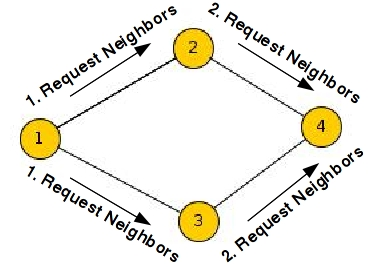
\includegraphics[width=0.25\textwidth]{../figures/sampling_error_arrows.jpg}
\label{fig:sampling_error_initial}}\hfill
\subfloat[node 4 sends its out-neighbors and fails]{
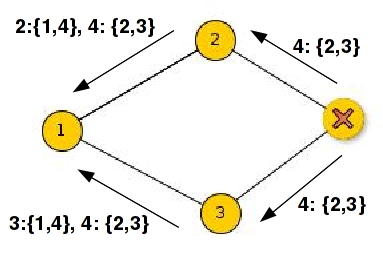
\includegraphics[width=0.25\textwidth]{../figures/sampling_error_arrows2.jpg}
\label{fig:sampling_error_final}}\hfill
\subfloat[adjacency matrix as computed by Node 1]{
\begin{tabular}[b]{l|cccc}
& 1 & 2 & 3 & 4\\
\hline 
1 & 0 & 1 & 1 & 0\\
2 & 1 & 0 & 0 & 1\\
3 & 1 & 0 & 0 & 1\\
4 & 0 & 1 & 1 & 0\\
\end{tabular}
\label{table:computed_matrix}} \hfill
\subfloat[real adjacency matrix]{
\begin{tabular}[b]{l|cccc}
& 1 & 2 & 3 & 4\\
\hline
1 & 0 & 1 & 1 & -\\
2 & 1 & 0 & 0 & -\\
3 & 1 & 0 & 0 & -\\
4 & - & - & - & -\\
\end{tabular}
\label{table:actual_matrix}}

\caption{In \ref{fig:sampling_error_initial}, node 1 requests a list of neighbors from each network node. All the nodes send their adjacency list to node 1, but while the lists are being transfered, node 4 fails as shown in \ref{fig:sampling_error_final}. As a result the adjacency matrix computed by node 1 is the one displayed in \ref{table:computed_matrix}, while the real adjacency matrix by the end of the sampling is shown in \ref{table:actual_matrix}
\label{fig:sampling_error}}

\end{figure}

There is a large number of decentralized networks used in practice. A typical example are systems that use a distributed hash table (DHT) to provide a lookup service of key-value pairs that is similar to a simple hash table, only spreading the pairs over nodes in the network based on some properties of both the nodes and the keys. Chord \cite{Stoica:2001:CSP:964723.383071} and Pastry \cite{Rowstron:2001:PSD:646591.697650} are two commonly used protocols that implement such DHT systems. Gnutella is also a very popular decentralized peer-to-peer network used by over 3 million users for file-sharing \cite{4146697} through clients like \textit{LimeWire} and \textit{Shareaza}.


\subsection{Network Overlays}
\label{subsec:overlay_diff}

The protocol that we propose in this project should be network-agnostic, in the sense that it should offer the capability to be applied in a wide range of networks, both physical and overlays, seamlessly. For this reason, it would be useful to briefly explain what a network overlay is and what are its differences and similarities to physical networks.\\

As an overlay network we generally define any virtual network topology that runs independently on top of some physical network, utilizing its infrastructure. From a logical point of view, an overlay network is very similar to physical networks, since it can be represented as a graph composed by a number of nodes that are connected to one another through either directed or undirected links or edges. The main difference of overlays from regular networks is that the nodes of the overlay can be thought as being connected by virtual links as Figure \ref{fig:overlay_network} illustrates. The black lines of the figure represent the links in a physical network, that actually connect nodes through some form of hardware, e.g. they could be Ethernet cables, optic fibers, coaxial cables etc. On the other hand, the yellow lines represent the logical links that are constructed by some overlay network, which in reality correspond to a path that could be composed by many physical links of the underlying network. \\

There is a wide range of overlays that are currently in existence, most of which run on top of the Internet. Some popular examples of overlay networks that are widely used in practice are peer-to-peer (P2P) networks, virtual private networks (VPN) and routing overlays like Skype for VoIP communications.  \\

Overlays are desirable in multiple occasions, since they allow network engineers and developers to design their own protocols and applications, which operate on top of an existing infrastructure, modifying its behavior to fit their needs. Since such a network is designed with specific goals in mind, it can be optimized to be more scalable and robust than a network of general purpose. For example, consider a file-sharing application operating over the Internet that uses an index to locate the files offered by users. If each participating node kept an index of its own shared files locally, then this would lead to an unbalanced network that would not be scalable for performing fast searches. If on the other hand an overlay was created that operated on top of the Internet and distributed the index keys uniformly amongst the participating nodes, the application would be more scalable, since any search would now require almost the same time.\\

On the other hand, overlays create several challenges that physical networks do not face due to their structure. First of all, since overlays are virtual networks, they have no control over the underlying physical network while at the same time they might even lack critical network information. For instance, a node in a physical network always knows which are its in and out-neighbors, through the physical network interfaces it controls, while a node of an overlay might lack some of these information, e.g. it might not know which nodes are considered its in-neighbors. Additionally, overlays do not always take into consideration the underlying network topology, resulting in inefficient utilization of network resources. For instance, nodes that are adjacent in an overlay, frequently exchanging messages, might actually be located multiple hops away from one another, generating traffic that is now spread throughout a large part of the network. Finally, since in most overlay networks all kind of users can join there are security concerns that need to be addressed, such as nodes generating malicious messages or refusing to comply with the protocol.


\begin{figure}[h]
\centering
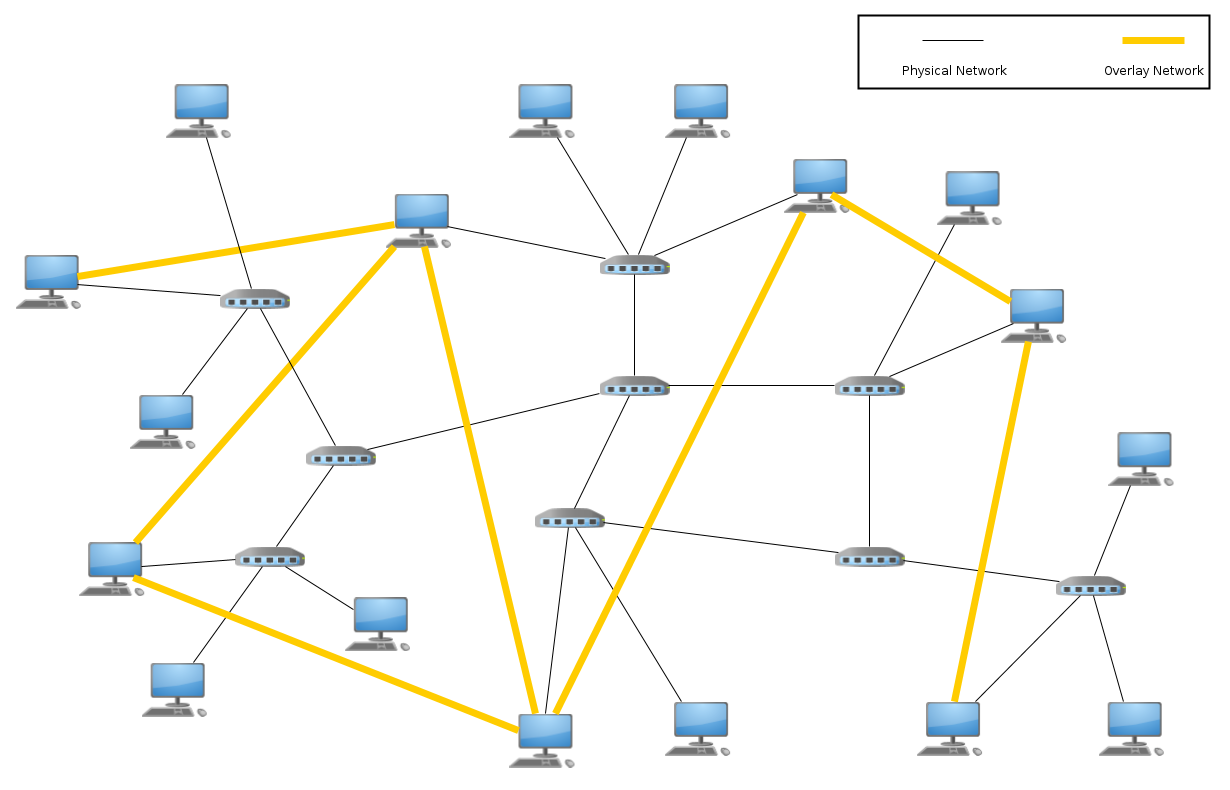
\includegraphics[width=0.9\textwidth]{../figures/network_overlay.png}
\caption{The thin black lines are links of the physical network, while the yellow lines are the virtual links of an overlay network.}
\label{fig:overlay_network}
\end{figure}

\subsection{Chord and Pastry}
\label{sec:pastry_chord}

This project aims at providing a protocol for computing the spectral properties of a wide variety of networks, both physical and overlays. It would thus be useful to briefly present two very popular peer-to-peer protocols, \textit{Chord} and \textit{Pastry}, that create network overlays in which our proposed protocol could potentially be deployed. Doing so, would allow us to locate the similarities that these networks share as well as their differences. This would provide us with a better understanding of our protocol's requirements as well as the restrictions posed to us. Additionally, these overlays could be used as a testbed for evaluating our results, and thus understanding how they operate would be important.



\subsubsection*{Chord}

Chord \cite{Stoica:2001:CSP:964723.383071} is a protocol for a peer-to-peer distributed hash table (DHT). Each Chord node stores key-value pairs for all the keys for which it is responsible. Every Chord node has as a unique ID its IP address. An important feature of the protocol is that all keys and IDs are assigned an $m$-bit identifier by hashing them using the SHA-1 algorithm \cite{Eastlake:2001:USH:RFC3174}, which is then used to perform all of the protocol's operations. There are two reasons for using the hash value as an identifier instead of the real values of keys and IDs. The first is that by hashing them, all the values belong to the same identifier space and can thus be referenced in the same manner. The second is that a hash function like SHA-1 uniformly distributes the keys and IDs to the network, greatly improving its performance and making it more robust.

\begin{figure}[h]
\centering
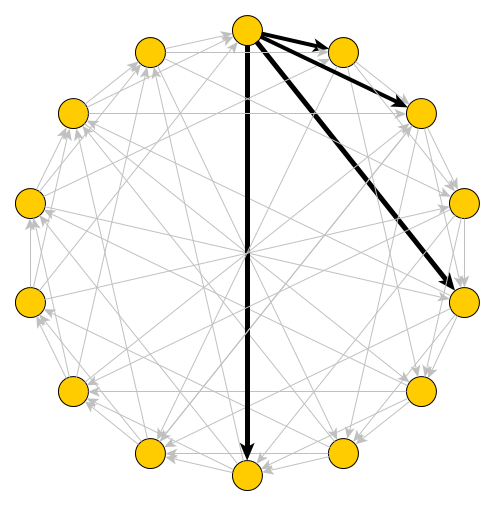
\includegraphics[width=0.6\textwidth]{../figures/chord.png}
\caption{The topology of a chord network overlay}
\label{fig:chord_overlay}
\end{figure}

Using their hashed identifiers the nodes are arranged in a circle of size at most $2^m$ as illustrated in Figure \ref{fig:chord_overlay}. The reason for this limitation in the number of participating nodes is that any ID or key can only be assigned a value from 0 to $2^m-1$. The hashed identifiers are placed in a clockwise incrementing manner in the ring and each node is assigned a successor and a predecessor, with which it can directly communicate. The successor of a node is the next node of the ring in a clockwise-direction and the predecessor is the previous one.
Any key $k$ is assigned to the node whose identifier is equal or follows the identifier of $k$. Due to the way that the identifiers are produced any node of the network will have at any time about $\frac{K}{N}$ keys, where $K$ is the total number of keys and $N$ is the number of nodes in the network. Apart from the successor and predecessor, every node keeps a $finger\ table$ which contains up to $m$ entries, with the $i^{th}$ entry of node $n$ being the IP of the node which is responsible for identifier $(n+2^{i-1}) mod 2^m$ (this means that the first entry in the finger table is its successor node).\\

When a node wishes to locate a value paired to a particular key $k$, it performs a search by using the nodes listed in its $finger\ table$, from the one that lies further away to the one that is closer. Using this method, the whole search process requires only $O(\log N)$ steps. The predecessor nodes are used only for maintenance purposes, i.e. for stabilizing the ring once a node joins/departs from the network.


 
\subsubsection*{Pastry}

Pastry \cite{Rowstron:2001:PSD:646591.697650} is also an overlay network for the implementation of a DHT similar to Chord. As in chord, every pastry node has a unique node id that is an 128-bit unsigned integer, produced by hashing the node's IP address or its public key. The nodes form a circular topology similar to chord based on the value of their ids. It is important to notice that since the ids are generated with the use of a hash function, the position that a node will have in the ring is irrelevant to its position in the physical network. For instance, two nodes that are adjacent in the physical network might be located in completely different locations within the Pastry ring. The keys stored in the overlay are also hashed by the same function to produce 128-bit values. For the purpose of routing, all node ids and keys are divided into digits, with each digit being $b$ bits long, yielding a numbering system of base $2^b$.\\

Every Pastry node maintains three data structures; a \textit{leaf set}, a \textit{neighborhood set} and a \textit{routing table}, which are used by the routing algorithm to locate the node that stores a particular key-value pair. The \textit{leaf set} contains the IP addresses of the nodes with the $l/2$ numerically closest larger node ids and the $l/2$ numerically closest smallest node ids, where $l$ is a protocol parameter that is typically set to 16. The \textit{neighborhood set} contains the $M$ closest peers in terms of some routing metric, which is defined by the user (e.g. the result of \textit{ping} or \textit{traceroute}). Finally, the \textit{routing table} is organized into $\lceil{\log _b N}\rceil$ rows with $2^{b-1}$ entries each, as illustrated in Figure \ref{fig:pastry_routing_table}. Each one of the entries in row $n$ of the routing table refers to a node that has the same $n$ first digits as the present node, but is different in the $n+1^{th}$ digit. Since there are a number of nodes that might have a particular prefix, the node that is closest to the present node, according to the routing metric, is chosen from the \textit{neighborhood set}.

\begin{figure}[h]
\centering
\subfloat[Routing table of a pastry node with id $75fax$, where $b=4$ and $x$ represents an arbitrary suffix]{
\fbox{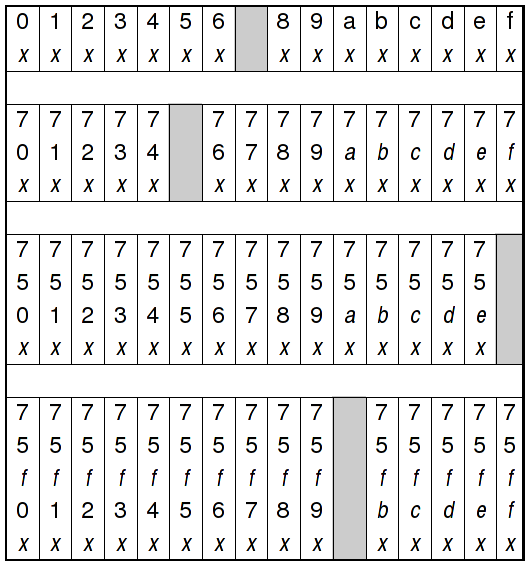
\includegraphics[width=0.4\textwidth]{../figures/pastry_table.png}}
\label{fig:pastry_routing_table}
}\hfill
\subfloat[Routing of a message with key $d46a1c$ from node with id $75fa12$]{
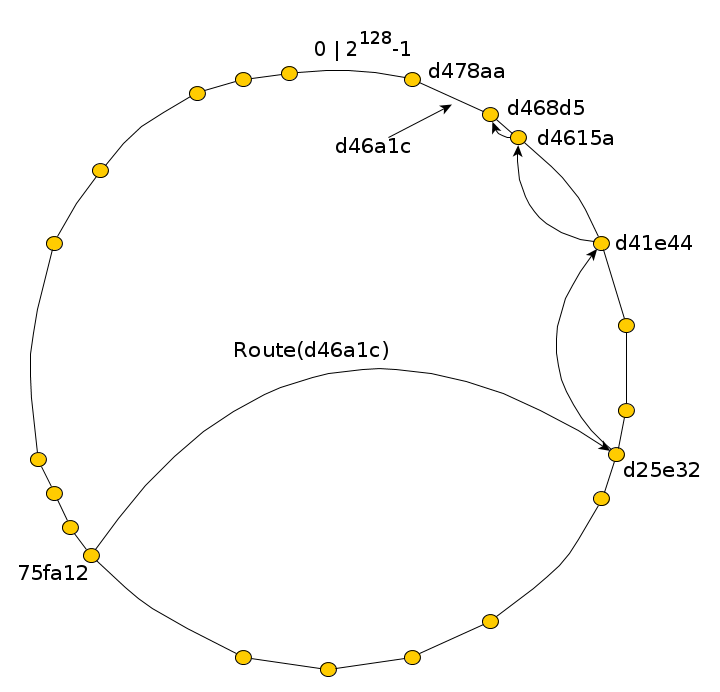
\includegraphics[width=0.45\textwidth]{../figures/pastry_routing.png}
\label{fig:pastry_routing_method}
}
\caption{Pastry overlay topology}
\label{fig:pastry_figures}
\end{figure}

When a node receives a request for a particular key $K$, it first checks its leaf set and forwards the request to the correct node if one is found. In the case that no such remote node exists, a check is performed by the local node to its routing table, trying to locate a node which shares a longer prefix with the requested key, than itself. In the case that no entry of the routing table satisfies this requirement, the node will forward the request to a peer from any of its tables (\textit{leaf set}, \textit{neighborhood set} or \textit{routing table}) that has a prefix of the same length as itself but whose full id is numerically closer to the destination. This means that all the nodes which could be contacted by any node for routing purposes in a Pastry ring are contained in the three aforementioned tables. Finally, a simplified version of Pastry was later proposed \cite{Castro:2003:TRS:1809315.1809337}, that completely removed the  \textit{neighborhood set}.


\section{Related Work}

In large scale decentralized networks there is often a need to know global state properties in order to deal with issues like maintenance, routing and quality of service. Since the aim of this project is to implement a system that samples for global network properties it would be useful to briefly present some related work. There has been a lot of research on computing global properties that can be broadly divided into three major categories; aggregation, sampling and spectral computation algorithms.

\subsection{Aggregation Algorithms}
\label{sec:aggregation_alg}

Aggregation acts as a summarizing mechanism of the overall state within the network. Each participating node shares some local information in the form of numerical values, that when combined can be used to infer global system information, which can in turn provide indicators that allow the evaluation of global network properties. Such indicators are very often desirable, since they can provide useful hints when attempting to ensure some level of performance, QoS etc \cite{Makhloufi:2009:DAP:1692742.1692756}. As an example consider a file-sharing network, where each node holds statistics like the size of all the locally stored files. An aggregation algorithm would provide an estimation of the whole network's average size of files, that could be a useful hint for calibrating the parameters that are relevant to the protocol used for transferring the files; e.g. a large average could mean that less file transfers should be made in parallel to avoid network congestion for a long time. Aggregation techniques can vary, from using simple aggregate functions (sum, max, average etc.) to more advanced like histograms \cite{Jurca:2009:CHL:1688933.1688991} and linear projections \cite{1662440}. Aggregation protocols can be further divided into two subcategories; gossip-based and tree-based aggregation schemes \cite{Makhloufi:2009:DAP:1692742.1692756}.

\subsubsection*{Gossip algorithms}

Gossip algorithms operate in rounds in an analogy to how gossip news spread in a social network. At each round nodes form pairs and exchange the values that they hold (e.g. the number of files stored on the disk of the node or the CPU-load). After a number of rounds, the values will have spread across the whole network like a virus, providing a good estimate of the global aggregate value. Due to the nature of gossip-based algorithms, they usually are simple, scalable and failure-resistant. However, every node needs to exchange and aggregate a large amount of data, resulting in high computation and communication costs.\\

Depending on the probability distribution used by a node to choose its pair, we can divide gossip algorithms in uniform \cite{Kempe:2003:GCA:946243.946317} and non-uniform \cite{Kempe:2004:SGR:1039488.1039491} \cite{Rabbat:2007:SGA:1524876.1525177}. Uniform algorithms are those in which nodes choose their pair uniformly and at random from the network or send a message that performs a random walk and terminates at some random node. \\

A fundamental uniform gossip-based algorithm proposed by Kempe et al. is \textit{Push-Sum} \cite{Kempe:2004:SGR:1039488.1039491}. The algorithm begins at round $i=0$, with each node $v$ maintaining a \textit{sum} $s_{v,i}$ and a \textit{weight} $w_{v,i}$. From that point on, every node executes Algorithm \ref{alg:push_sum} for $t$ rounds, sending at each round its current estimation to one of its out-neighbors. \\
 
\begin{algorithm}
\caption{Push-sum algorithm at node $v$}
\label{alg:push_sum}
\begin{algorithmic}[1]

\STATE $s_{v,0} \leftarrow x_v$ \COMMENT {Node $v$ holds an initial value $x_v$}
\STATE $w_{v,0} \leftarrow 1$
\STATE Send the pair $\{s_{v,0}, w_{v,0}\}$ to yourself
\FOR{$i=1 \dots t$}
\STATE $s_{v,i} = \sum_{r} \hat{s}_{u, i-1}$ \COMMENT {$\hat{s}_{u, i-1}$ are the values sent by any node $u$ to $v$ in the previous round}
\STATE $w_{v,i} = \sum_{r} \hat{w}_{u, i-1}$ \COMMENT {$\hat{w}_{u, i-1}$ are the weights sent by any node $u$ to $v$ in the previous round}
\STATE $\hat{s}_{v,i} \leftarrow \frac{1}{2}s_{v,i}$
\STATE $\hat{w}_{v,i} \leftarrow \frac{1}{2}w_{v,i}$
\STATE Choose target $f_t(i)$ uniformly at random by out-neighbors
\STATE Send the pair $(\hat{s}_{v,i},\hat{w}_{v,i})$ to $v$ (yourself) and $f_t(i)$
\STATE The estimate of the average in step $i$ is $\frac{s_{v,i}}{w_{v,i}}$
\ENDFOR

\end{algorithmic}
\end{algorithm}

This algorithm can also be used to compute sums instead of averages, simply by setting the weight $w_{v,0}$ to 1 only in one node and 0 to the rest. An interesting property of the algorithm is that, assuming that no failures occur, it will converge if executed for a sufficiently large number of steps. The convergence speed is related to a number of parameters including the size and topology of the network and the communication mechanism used for exchanging the messages.  \\

On the other hand, nodes in non-uniform gossip algorithms choose their pairs in a biased manner, showing preference to those that have some desirable properties. For instance \textit{Spatial gossip} \cite{Kempe:2004:SGR:1039488.1039491} \cite{Rabbat:2007:SGA:1524876.1525177} is a non-uniform algorithm, in which the selection of nodes is done according to their distance, with nearby nodes being chosen more often than those that are far away, reducing the network delays and improving the speed of execution. A pitfall of non-uniform algorithms is that if not designed properly, they can lead to bad estimates due to network partitioning. For example, consider the network of Figure \ref{fig:non_uniform}. The numbers in the nodes represent the values that each node initially has and the dotted line represents a link of great distance between two nodes. If a non-uniform algorithm is used that completely ignores nodes that are very far away, the network ends up with two partitions (yellow and gray) that are disjoint and make completely different estimations of the aggregate value, since they are not taking into account any of the values present in the other partition. However, if non-uniform algorithms are carefully designed, they can be faster and more efficient than those that are purely random. 

\begin{figure}[h]
\centering
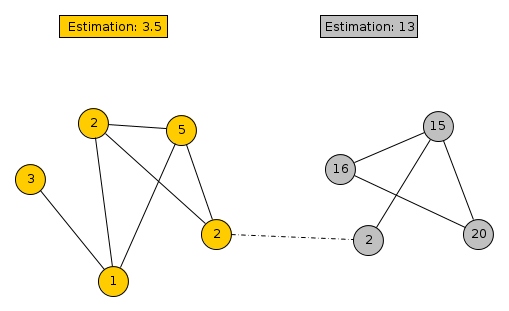
\includegraphics[width=0.9\textwidth]{../figures/non-uniform.png}
\caption{A network partitioned by a non-uniform gossip algorithm}
\label{fig:non_uniform}
\end{figure}




\subsubsection*{Tree-based algorithms}

Tree-based algorithms compute aggregates by using trees in a bottom-up fashion. Typically a node that initiates the protocol makes a request to build a spanning tree on the network (e.g. by using BFS) and then aggregate values are computed and propagated to the higher levels of the tree, achieving lower communication costs compared to gossip-based algorithms. \\

The simplest tree-based algorithm is \textit{SingleTree} \cite{Bawa03estimatingaggregates}, that works in two phases as illustrated in Figure \ref{fig:simpletree}. During the first phase, the node that needs to perform a query broadcasts an initiation message to the network and a spanning tree is built, in which each node $v$ sets as its parent the node $u$ that first transmitted the initiation message to $v$. In the second phase, the query is computed by aggregating the nodes' values through the spanning tree. A node will send the values it has collected to its parent only once it has received an answer containing a value from all of its children. While this algorithm is very simple it has the disadvantage of being very sensitive to failures. If a node $u$ crashes after it has communicated with its children and before it manages to send the values it collected to its parent, all the information provided by the nodes of the subtree that has as a root $u$ will be lost (Figure \ref{fig:spanning3}) and the tree needs to be reconstructed for a proper value to be computed. 

\begin{figure}[ht]
\centering
\subfloat[][]{
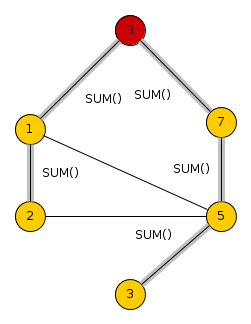
\includegraphics[width=0.25\textwidth]{../figures/spanning1.png}
\label{fig:spanning1}}\hfill
\subfloat[][]{
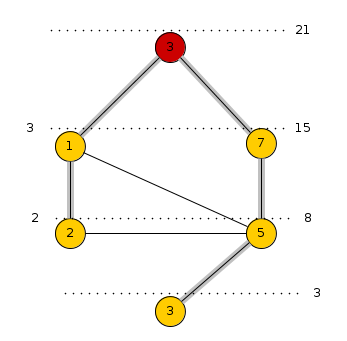
\includegraphics[width=0.33\textwidth]{../figures/spanning2.png}
\label{fig:spanning2}}\hfill
\subfloat[][]{
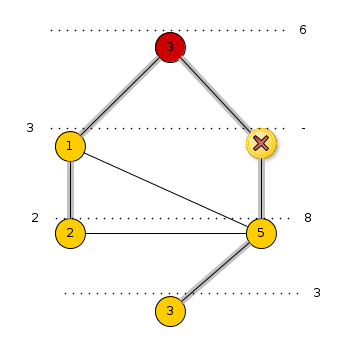
\includegraphics[width=0.33\textwidth]{../figures/spanning3.png}
\label{fig:spanning3}}

\caption{In \ref{fig:spanning1}, the  red querying node requests a \textit{sum} aggregate function and the spanning tree is constructed (thick gray lines). In \ref{fig:spanning2} each node propagates to the higher level the aggregated values it collected. In \ref{fig:spanning3} the node with the red X fails before sending the values it gathered, resulting in the computed value at the querying node being 6 instead of 21.}
\label{fig:simpletree}

\end{figure}

As an enhancement that tackles the aforementioned problem, Bawa et al.\cite{Bawa03estimatingaggregates} propose \textit{MultipleTrees}, where instead of just one, $k$ minimum spanning trees are constructed using BFS, all rooted at the node that performed the query. Again, the querying node sends an initiation message to all the nodes. Every node $u$ has a variable $l(u)$ that is associated with the level which $u$ will have on the spanning trees. A node $v$ that received the initiation message directly from the querying node will have $l(v)=1$, while any other node $w$ will have $l(w)=l(r)+1$, where $l(r)$ is the value of the first node $r$ from which $w$ received a message. Additionally each node $u$ will hold a set $S$ containing all the nodes $v$ it has seen, for which $l(v)<l(u)$. When the initiation phase terminates, all nodes will choose $k$ nodes from $S$ as their parents for the $k$ spanning trees. In the second phase, each node propagates its collected values to its parents. This algorithm is more robust compared to \textit{SingleTree}, since even if a node fails, there are additional spanning trees, where the failed node might be in a lower level (e.g. a leaf) and thus the results might be more precise.


\subsection{Sampling Algorithms}

In this category we find algorithms that try to infer global network properties by performing projections in local properties acquired by sampling a subset of the network nodes. If the selected nodes are chosen consistently, then a good estimation of the actual values could be computed.\\

A well-known sampling technique, used for estimating some statistics of an undirected network is \textit{Random Tour}\cite{Massoulie:2006:PCS:1146381.1146402}. The idea is that any node $i$ that wishes to make an estimation of some global value, initializes a counter $X$ to the value $\phi(i)/d(i)$, where $d(i)$ is the degree of $i$ and $\phi(i)$ is any function that produces the wanted value at $i$, e.g. if every node $j$ sets $\phi(j)=1$, then the algorithm will make an estimation of the size of the network. The initiator node sends a message containing $X$ to perform a random tour of the network, that is, to visit neighboring nodes, chosen uniformly at random, until it reaches the initiator node for a second time. Every node $j$ that receives this message, increments $X$ by a value $\phi(j)/d(j)$ and in the end, the initiator node $i$ makes an estimation of the wanted property by computing the value $Xd(i)$. An advantage of this algorithm is that it is guaranteed to produce unbiased estimations, however it scales linearly with network size, meaning that it can only be applied efficiently in small to moderate networks.\\

Another sampling technique, used for network size estimation is called \textit{BdayParadox} \cite{Bawa03estimatingaggregates}. This technique is based on the birthday paradox, i.e. if a population of size $n$ is sampled repeatedly with replacement and uniformly at random, then the number of trials required before a value is sampled twice will have an expected value of $\sqrt{n}$. \cite{Motwani:1995:RA:211390}. Using this property, the algorithm randomly samples network nodes and keeps track of the number of samples acquired before a collision is recorded. Then, if $X_r$ is the number of nodes sampled, the size of the network can be estimated as $\bar{n}=\frac{X_r^2}{2}$. The samples for this method are taken by performing discrete time random walks of length $r$, i.e. the querying node initiates a random walk that lasts for $r$ hops and the value of the node that is the last in the walk is taken as a sample. \\

A problem that the aforementioned method presents is that discrete time random walks can suffer from bias whenever peers have unequal degrees. An algorithm that deals with this problem is \textit{Sample and Collide} \cite{Massoulie:2006:PCS:1146381.1146402}. This algorithm relies in continuous time random walks to take the samples. The querying node initializes a timer $T$ in a sampling message and sends it off in a random walk. Any node $i$ which receives the sampling message picks a random number $R$ uniformly distributed in [0,1] and decrements $T$ by $\log(R)/d(i)$, where $d(i)$ is the degree of $i$. The node in which the timer will have a value $T\leq0$ will be the one to send a sample to the initiator. Both \textit{BdayParadox} and \textit{Sample and Collide} are sub-linear methods, which allows them to be used into large-scale networks. 

\subsection{Spectral Computation Algorithms }

While the algorithms presented in the previous sections can be very useful for producing simple network statistics and in most cases can be easily implemented, the information they provide us are network independent and they do not map properties related to the structure and the connectivity of the network \cite{6195806}. For instance in a file-sharing network, \textit{Push-sum} could give us an estimation of the size of the network, however there is nothing it could tell us about the network's topology (e.g. whether the network has a particular structure or  if it is random). \\

The spectral computation algorithms achieve exactly this by analyzing the spectrum of the network graph. The general idea behind all spectral algorithms is that they attempt to compute all or the most significant eigenvectors and eigenvalues of a matrix describing or being somehow closely related to the structural properties of the network, which is distributed among the network's nodes. Common examples of matrices used are the adjacency matrix that marks neighboring nodes and the transition probability matrix that holds the probabilities of going from any node $i$ to some other node $j$. The eigenvectors and the eigenvalues of such matrices can provide important structural information. For instance using the second largest eigenvalue of some network's transition probability matrix, we can compute its mixing time \cite{Snader:2009:ESP:1855663.1855672} \cite{Datta:2007:UDS:1270387.1270884}, that is, the necessary length of a random walk required to compute the steady state probabilities of the network. While such a network property might not appear to be useful by itself, it can be used as a parameter to compute the cost and precision of other methods like aggregation algorithms. \cite{Kempe:2003:GCA:946243.946317} \cite{Sauerwald:2007:MEE:1781574.1781600}.\\
 
 
There is a large number of algorithms which obtain information from the network's spectral properties. Kempe and McSherry \cite{Kempe:2004:DAS:1007352.1007438} propose a decentralized, distributed algorithm for computing the top-$k$ eigenvectors of a symmetric matrix and singular vectors of arbitrary matrices that are distributed across the network, by using a decentralized version of \textit{Orthogonal Iteration}(\textit{OI}). In the original method, $k$ random vectors are chosen for the initialization round before the algorithm performs a number of iterations. The first step of every iteration is to multiply the vectors by $A$, where $A$ is the weighted adjacency matrix under consideration. The resulting vectors are then orthonormalized and are used as an input for the next iteration. This algorithm terminates once the vectors converge. The difference of the distributed version lies in the way the orthonormalization is performed. In the original \textit{OI} the orthonormalization is usually performed by computing the QR factorization of the vectors. In the distributed version, \textit{Push-sum} is used to estimate a matrix $K$ which is factored by each node to compute the orthonormalization matrix. While this algorithm can be very useful for analyzing the structural properties of large networks by providing the most significant eigenvectors and eigenvalues, the amount of data that are exchanged during the iteration steps could lead to high traffic and eventually network congestion.\\


\textit{EigenSpeed}  \cite{Snader:2009:ESP:1855663.1855672} and \textit{EigenTrust}  \cite{Kamvar:2003:EAR:775152.775242} are also algorithms that are based in computing spectral properties of the network. \textit{EigenSpeed} uses the principal eigenvector of a matrix of bandwidth observations of the network to estimate the bandwidth capacity of nodes. \textit{EigenTrust} is a reputation management algorithm for peer-to-peer networks, which computes the principal eigenvector of a matrix $C$ containing trust values of the network's nodes using a distributed power method. The elements of the computed eigenvector represent the global trust values of the nodes and could be useful as a directive of whether the nodes should trust the content that a remote node has to offer or not. Additionally, both methods also take into account malicious nodes that could present wrong values to tamper with the results of the computation. It should also be mentioned, that the decentralized algorithm used as the basis of the protocol proposed in this project also belongs in the category of spectral computation algorithms and will be analyzed in greater depth in the following section.


\section{A Decentralized Algorithm for Estimation of Global Properties}
\label{sec:decentralized_algo}

In this section we make a detailed presentation of the decentralized spectral computation algorithm by Carzaniga et al. \cite{6195806} which forms the basis of our proposed protocol. This algorithm uses classic methods from system identification and realization to compute a matrix closely related to the network's adjacency matrix, which can provide us with some very useful network properties, like its mixing time and spectral gap. Therefore it would be useful, before discussing the details of the algorithm, to make a short introduction to dynamic systems and realization algorithms, to better understand how the proposed method works. Finally, we make a brief presentation of the algorithm's evaluation results as well as its limitations.

\subsection{Dynamic Systems}

A dynamic system is any physical or artificial system that evolves over time and whose behavior is described by taking time as a parameter \cite{luenberger1979introduction}. In order to define a dynamic system we need a time index, a description of the states of the system and a set of rules, called \textit{dynamics}, by which the state of the system evolves in time. In a mathematical language, the \textit{dynamics} would be a function that maps a state into another. As a simple example, consider our own solar system. A state of this system would be the positions and velocities of all the planets and the sun at a given time and the \textit{dynamics} for state evolution would be the laws of gravity. Using these laws, we could predict the positions and velocities of the planets at any given time in the future.\\

A dynamic system can have zero, one or more inputs and outputs. An input, also called an \textit{impulse}, originates outside the system and does not depend on what happens in it, but affects its state evolution, i.e. the new state now depends on both the previous state and the given input. On the other hand, outputs, or \textit{impulse responses} are generated by the system through some function that depends on the previous state and possibly the given input. 

\begin{figure}[h]
\centering
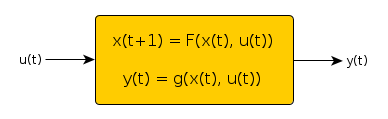
\includegraphics[width=0.6\textwidth]{../figures/dynamic_system.png}
\caption{An input-output dynamic system at time $t$, where $u$ is the input, $y$ is the output and $F$ and $g$ are functions changing the state of the system and computing the output respectively}
\label{fig:dynamic_system}
\end{figure}

Depending on their characteristics, we can use various classifications for dynamic systems:

\begin{description}
  \item[Linear versus Nonlinear] \hfill \\
   Linear dynamic systems are systems with linear evaluation functions, that obey the principles of superposition and homogeneity. In this type of systems, given a state and some input, we can always find an exact solution for the new state and the output. On the other hand, nonlinear dynamic systems do not hold that property and their behavior can be completely unpredictable.
  \item[Time-variant versus Time-invariant] \hfill \\
    A system is considered time-invariant if its parameters do not change with time. Formally, if an input $u(t)$ of a time-invariant system produces some output $y(t)$ at some time $t$, then the same input $u$ at some future time $t+\delta$, for $ \delta \ge 0$ will give the time shifted output $y(t+\delta)$. A common example of a time-invariant system is an electronic amplifier, since the same input signal will always produce the same output signal regardless of time. On the contrary, the parameters of a time-variant dynamic system change with time. As an example, consider a dynamic system describing the mass of a car, which changes with time, as fuel burns.
  \item[Continuous-time versus Discrete-time] \hfill \\
   The evolution of the system can occur smoothly over time or in discrete time steps. In the former case, we call this a continuous-time dynamic system, while in the latter we call it discrete-time. If $t$ is the time variable, we could consider the discrete-time as taking snapshots of the system state at fixed intervals, with $t = 0,1,2,3,\dots$, while the continuous-time would be like taking snapshots of the system state at any moment $t \geq 0$. Both continuous and discrete-time systems can be linear or nonlinear and time-variant or invariant.
\end{description}


In the context of this project we are interested in a discrete-time, linear, time-invariant, single-input-single-output model, that is defined by the following equations:


\begin{eqnarray}
x(t+1) = Ax(t)+Bu(t) \label{eq:one} \\
y(t)=Cx(t)   \label{eq:two}
\end{eqnarray}

where $x(t) \in \mathbb{R}^n$ represents the state of the system at time $t$, $u(t) \in \mathbb{R}$ is the input at time $t$ and $y(t) \in \mathbb{R}$ is the output. $A \in \mathbb{R}^{n \times n} $ is the state-transformation matrix, $B \in \mathbb{R}^n$ is a vector used for mapping the input to the state of the system and $C \in \mathbb{R}^n$ is a vector used for mapping the state to the output. The size $n$ of $x$ is also called the $order$ of the system. The impulse response of the system at time $t=0$ will be $h(0)=0$ and $h(t)=CA^{t-1}B$ for $t=1,2,3\dots$.



\subsubsection{Kung's Realization Algorithm}
\label{sec:kung}

A realization algorithm is a system identification technique which can generate a system realization by using impulse response data. Given the impulse responses of a dynamic system we can identify their modal parameters. For instance, feeding the impulse responses of the dynamic system described in the previous section in a realization algorithm, we could identify matrix $A$ and vectors $B$ and $C$ of equations \ref{eq:one} and \ref{eq:two}.\\

\noindent Kung proposes an approximate realization algorithm, which identifies the parameters of a system of order $n$ using $2n-1$ impulse responses  \cite{1992040} \cite{1164997}. The algorithm determines a reduced model of order $p \le n$ and fits the triple $[A, B, C]$ to the impulse responses provided. The steps of the algorithm are the following: \\

Given $2n-1$ impulse responses $h(1), h(2), \dots h(n-1)$, construct an $n \times n$ Hankel matrix:\\

$H = \begin{bmatrix}
       h(1) & h(2) & h(3) & \cdots & h(n) \\
       h(2) & h(3) & h(4) & \cdots & h(n+1) \\
       \vdots & \vdots & \vdots & \ddots & \vdots \\
       h(n) & h(n+1) & h(n+2) & \cdots & h(2n-1)
     \end{bmatrix}
$\\

and perform singular value decomposition (\textit{SVD}) \cite{citeulike:2342309}, i.e.,

\begin{equation}
H = USV^T
\end{equation}

where $U$ and $V$ are $n \times n$ orthogonal matrices and $S$ is an $n \times n$ diagonal matrix containing in its diagonal the singular values $s1, s2, \dots, sn$ of $H$ in decreasing magnitude. The singular value decomposition of $H$ can also be expressed as \\\\

$H = \begin{bmatrix}
U_1 & U_2 
\end{bmatrix}
\begin{bmatrix}
S_1 & 0 \\
0 & S_2
\end{bmatrix}
\begin{bmatrix}
V_1^T \\
V_2^T
\end{bmatrix}
$\\\\


where $U_1$ contains the first $p$ columns of $U$, $U_2$ the last $n-p$, $V_1$ contains the first $p$ columns of $V$ and $V_2$ the last $n-p$. Finally, $S_1$ is a $p \times p$ sub-matrix of $S$, composed of the $p$ largest singular values of $H$ in its diagonal and $S_2$ an $ (n-p) \times (n-p)$ sub-matrix of $S$, containing in its diagonal the $n-p$ smallest singular values of $H$.Then, $A$ can be computed as  

\begin{equation}
A = G_1^{-1}G_2
\end{equation}

where $G_1$ and $G_2$ are obtained from $U_1S_1^{\frac{1}{2}}$ as the first and the last $2n-2$ rows, respectively.\\

The order $p$ of the approximation can be any integer $0 \le p \le n$ and a usual approach into choosing $p$ is to set a threshold to the singular values of $H$. $p$ will then be the number of the singular values that are above this threshold. For instance, the threshold could be $cs_1$, where $s_1$ is the dominant singular value of $H$ and $c \in \mathbb{R}$ some small constant, e.g. $ 0.01$.

\subsection{Algorithm Overview}

The decentralized algorithm proposed by Carzaniga et al. \cite{6195806} can be applied in computer networks that fulfill certain requirements. A network of size $n$ can be represented as a graph $G$ of $n$ vertices, where each vertex represents a node and each edge a unidirectional network link (a bidirectional connection requires two edges). Then, $G$ should be strongly connected and aperiodic and the network should be of a low diameter $\varDelta << n$ and low maximum degree $d$. These requirements are reasonable for many types of networks as for instance peer-to-peer networks usually have a diameter of $\varDelta = \mathcal{O}(\log n)$ \cite{1258114}\cite{Rowstron:2001:PSD:646591.697650}\cite{Stoica:2001:CSP:964723.383071} \cite{citeulike:92971} \cite{Schlosser:2002:HHO:1756247.1756261} .\\

The idea behind the algorithm is that we can model a network fulfilling the aforementioned requirements as a dynamic system like the one described by Equations \ref{eq:one} and \ref{eq:two}. Matrix $A$ could be any matrix closely related to the adjacency matrix of graph $G$, as long as its elements can be produced by information held locally by the network nodes, so that each node can compute and store a part of $A$. Any matrix $A$ is considered related to the adjacency matrix of $G$ if $a_{uv} \ne 0$ only if $u=v$ or there is an edge from node $v$ to node $u$. An important notice is that an edge $(v,u)$ is stored at position $(u,v)$ of the matrix, as Figure \ref{table:adjacency_matrix} illustrates, for consistency with Equations \ref{eq:one} and \ref{eq:two}, resulting at each node $v$ storing the $v^{th}$ column of $A$, instead of storing a row, as most relevant models do. As an example consider the small network illustrated in Figure \ref{fig:modeled_network}. For the model of this network, $A$ is the transition probability matrix with $a_{uv}$ being equal to the probability of going from node $v$ to node $u$ when performing a random walk in the network. It is easy to see that this matrix will have zero elements only to those positions that the adjacency matrix will be 0. The probability distribution of any node can be different (uniform or non-uniform) and it depends on the type of the modeled network.\\

\begin{figure}[h]
\centering
\subfloat[The modeled network]{
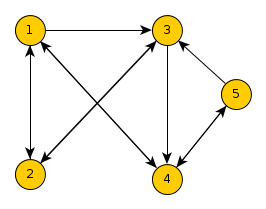
\includegraphics[width=0.25\textwidth]{../figures/example_network.png}
\label{fig:modeled_network}}\hfill
\subfloat[Adjacency matrix of the network]{
\begin{tabular}[b]{l|ccccc}
& 1 & 2 & 3 & 4 & 5\\
\hline 
1 & 0 & 1 & 0 & 1 & 0\\
2 & 1 & 0 & 1 & 0 & 0\\
3 & 1 & 1 & 0 & 0 & 1\\
4 & 1 & 0 & 1 & 0 & 1\\
5 & 0 & 0 & 0 & 1 & 0\\
\end{tabular}
\label{table:adjacency_matrix}} \hfill
\subfloat[Matrix A. Each column sums to 1]{
\begin{tabular}[b]{l|ccccc}
& 1 & 2 & 3 & 4 & 5\\
\hline 
1 & 0 & 0.7 & 0 & 0.2 & 0\\
2 & 0.33 & 0 & 0.5 & 0 & 0\\
3 & 0.33 & 0.3 & 0 & 0 & 0.5\\
4 & 0.33 & 0 & 0.5 & 0 & 0.5\\
5 & 0 & 0 & 0 & 0.8 & 0\\
\end{tabular}
\label{table:matrixA}}
\caption{Simple model network and adjacency-related matrices}
\label{fig:modeled_network_example}
\end{figure}

The purpose of the algorithm is for each network node to produce an estimate of the dominant eigenvalues of matrix $A$ by gathering impulse responses in a number of rounds. The computed eigenvalues could then be used to determine a number of spectral network properties. The properties that can be computed, depend on how we define matrix $A$. For instance, the second eigenvalue of the transition probability matrix can be used to compute the \textit{mixing time} of the network.\\

The steps required can be seen in Algorithm \ref{alg:basic}. Each node $v$ holds one column $a_v$ of matrix $A$, containing the local information related to the adjacency matrix.

\begin{algorithm}
\caption{estimation algorithm at node $v$}
\label{alg:basic}
\begin{algorithmic}[1]

\STATE $x_v \leftarrow$  Choose a value uniformly from $\{0,1\}$
\STATE $h_v(1) \leftarrow x_v$
\FOR{$t \leftarrow 2 \dots k$}

\FOR{$u \in$ out-neighbours$(v)$} 

\STATE send value $x_{v}a_{uv}$ to $u$
\STATE collect all values $w$ sent by in-neighbors
\STATE $x_v \leftarrow \sum{w}$
\STATE $h_v(t) \leftarrow x_v$

\ENDFOR

\ENDFOR
\STATE $\hat{A_v} = $ Kung's realization with $h_v(1),\dots, h_v(k)$
\STATE compute the dominant eigenvalues of $\hat{A_v}$
\STATE exchange the eigenvalues with neighbors
\STATE collect estimates from neighbors
\STATE adjust estimates to the median of the collected estimates

\end{algorithmic}
\end{algorithm}

In the beginning, each node must randomly select a value from 0 and 1 as the initial impulse. At each of the following rounds, every node computes locally $x_v a_{uv}$ and sends it to all its out-neighbors. Then, node $v$ updates its value $x_v$ by adding all the values received by its in-neighbors. This value is also stored as $h_v(t)$, i.e. the impulse response of node $v$ in round $t$.\\

As already stated, every node holds only partial information of matrix $A$ (one column each). However, to analyze it's spectrum, the whole matrix is required. Using the impulse responses gathered in the previous phase, $A$ or an approximation of $A$ of lower order can be computed by using Kung's approximate realization algorithm. As mentioned in Section \ref{sec:kung}, Kung's algorithm requires $2n-1$ impulse responses in order to realize a system of order $n$, which means that for an exact estimation of a network of size $n$, the number of rounds required by Algorithm \ref{alg:basic}, would normally be $k=2n-1$. However, Carzaniga et. al argue, that for a network fulfilling the requirements set in the beginning of the section (strongly connected, aperiodic, with low diameter and of low degree), shorter impulse responses in the order of the diameter of the network rather than its size, should be enough to provide a valid approximation. Using the approximation $A_v$ of matrix $A$ computed in this step, we can then proceed and find its dominant eigenvalues.\\

A problem that arises at this point is that nodes across the network can observe different systems (gather different impulse responses) and as a result compute different realizations and spectral estimations with different levels of accuracy. To make the results of the algorithm more accurate and uniform, an additional round is performed, where each node sends its estimated eigenvalues to all of its out-neighbors and then the final estimation of each node is computed by finding the median of all the available values. This round reminds the way gossip algorithms behave, so it could be called the \textit{gossip round}.

\subsection{Evaluation results and Limitations}

This algorithm was evaluated in a simulated synchronous environment for various types of networks and overlays (e.g. Chord) using a uniform transition probability matrix as matrix $A$, i.e. all the edges coming out of a node $v$ have the same probability $1/degree(v)$. The evaluated network properties were the network's \textit{spectral gap} and its \textit{mixing time}. The \textit{spectral gap} is defined as $|\lambda_1 - \lambda_2|$, where $\lambda_1$ and $\lambda_2$ are the two eigenvalues of the approximate matrix $A_v$ with largest moduli. Since the transition probability matrix is stochastic (all columns sum to 1), the first eigenvalue is always 1. Thus the \textit{spectral gap} can be computed by $1-|\lambda_2|$. The \textit{mixing time} can be approximated by $t_{mix} = \log _{|\lambda_2|}\epsilon$, where $\epsilon$ is the desired error \cite{Datta:2007:UDS:1270387.1270884} \cite{Snader:2009:ESP:1855663.1855672}.\\

In general, the algorithm performs well producing accurate estimates of the \textit{mixing time} and \textit{spectral gap} with a short number of impulse responses for very large networks (10000 nodes), when no failures occur. However, in unstable networks, where even one failure occurred, the results of the evaluation revealed large estimation errors that could go as high as $200 \%$. Additionally, the estimation incurred a small fixed error that seems to be independent of the number of impulse responses used. Finally, it should be noted that this algorithm does not take into account malicious nodes, i.e. the algorithm would not work properly if a node refused to cooperate and send the values it computed to its out-neighbors or if the values it sent were intentionally malformed. 


\chapter{Protocol Design}
\label{sec:design}

In this chapter we present the design requirements that our proposed protocol should fulfill, discussing advantages and disadvantages that certain design decisions might incur to the applicability and efficiency of our proposal. Moreover, we present an in-depth analysis of the proposed protocol. Finally, this section discusses the design and architecture of our implementation, presenting its constituent components at a high level. The goal is to allow the reader to understand how our implementation attempts to satisfy the requirements set in a simple manner, before discussing its details in Chapter \ref{sec:implementation}.

\section{Model Assumptions}
\label{sec:model_assumptions}

The first step before proceeding in presenting our proposed protocol and an overview of the implementation, is defining a model for the network, which will provide us with an abstract representation of important properties and relationships and  will give us an insight about its applicability in different types of real-life networks. \\

We model the network as a directed graph $G = (V,E)$, where $V$ is a set of vertices and $E$ is a set of edges. A vertex can be interpreted as a node (e.g. a workstation in the network) and an edge as a link or a channel between two nodes. In addition the graph is dynamic in the sense that vertices and edges can be added or removed, as nodes join in and depart from the network.\\

Since the network is represented by a directed graph, communications are by default unidirectional. Thus a bidirectional communication is represented as two independent unidirectional channels with the use of two edges. The use of unidirectional communications is very important for our model, since it allows us to define and distinguish the type of neighbors that each node can have to \textit{in-neighbors} and \textit{out-neighbors}. We say that a node $u$ is an \textit{in-neighbor} of $v$, if there exists an edge $(u,v) \in E$ and that a node $u$ is an \textit{out-neighbor} of $v$ if there exists an edge $(v,u) \in E$, as illustrated in Figure \ref{fig:neighbors}. A requirement that Algorithm \ref{alg:basic} presented in Section \ref{sec:decentralized_algo}, is for the analyzed graph to be strongly connected. This means that every node of the network needs to have at least one \textit{in-neighbor} and one \textit{out-neighbor}.\\


\begin{figure}[h]
\centering
\subfloat[The gray nodes are the \textit{in-neighbors} of $v$]{
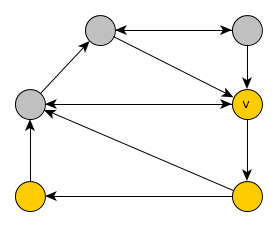
\includegraphics[width=0.4\textwidth]{../figures/in_neighbours.png}
\label{fig:in_neighbors}}\hfill
\subfloat[The blue nodes are the \textit{out-neighbors} of $v$]{
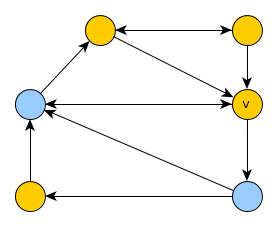
\includegraphics[width=0.4\textwidth]{../figures/out_neighbors.png}
\label{fig:out_neighbors}}

\caption{In and out-neighbors of a node}
\label{fig:neighbors}

\end{figure}

This model can be used to represent any network topology that our protocol should support. However, in order to make the model more realistic, we need to discuss in greater depth our assumptions about the communication medium used, the kinds of failures that might occur both in nodes and in links and the synchrony model that should be adopted. 


\subsubsection*{Synchrony Considerations}

One of the most important parameters that should be defined is whether the protocol will be deployed in a synchronous or an asynchronous environment. In a synchronous environment, there is a known upper bound in computations and communication steps, with nodes having perfectly or approximately synchronized physical clocks. Such a model would allow our protocol to operate in timed rounds and would greatly simplify all of its required actions. For instance, every node would know exactly which messages to expect by its neighbors in each time-slot and would not have to worry about received messages being out of order and probably being ignored in previous rounds.\\

On the other hand, an asynchronous environment gives no time guarantees, with processes not having even approximately synchronized clocks. In an asynchronous environment, every node could be in a different round than the rest. When all the messages required for some round have been received or the node has identified its neighbors as failed, it proceeds to the next round computing a new impulse response and sending messages to its out-neighbors. This means that any node could receive messages for future rounds, which should somehow be managed in order to be used when required. Obviously, the second approach is a lot more challenging than assuming that the network is synchronous. However, for any general network, the asynchronous model seems a more reasonable choice, as having synchronized clocks in large networks is not usually easily achievable and in fact you would never expect highly diverse networks, like peer-to-peer, to exhibit such a property. \\

\subsubsection*{Communication Medium}

Communications in the network are achieved by message passing through the predefined channels. For the requirements of our protocol it is absolutely necessary that the unicast operations of \textit{send()} and \textit{receive()} are supported by the network, for sending and receiving the values $x_va_{vu}$ as described in Algorithm \ref{alg:basic}. Additional support for a \textit{broadcast()} operation could be useful for the protocol initialization (i.e. let all the participating nodes know that a new sampling has been requested), however, our proposal does not make use of it, making the existence of a broadcast operation unnecessary.\\

Sending and receiving of messages should be non-blocking operations. The reason for this choice, is that since this is an asynchronous model, every node might be in a different round than the rest and a blocking operation could make the whole protocol inefficient. For instance, consider a network using the decentralized algorithm by Carzaniga et. al, where a node $u$ is in round $k=5$ and its \textit{out-neighbors} are still in round $k=3$, waiting for some values as illustrated in Figure \ref{fig:sending_operation}. Once round 5 is over for $u$, it computes the new impulse response $h(5)$ and begins sending values $x_ua_{vu}$ to all of its \textit{out-neighbors} $v$ for round 6. If the \textit{send()} operation was blocking, then $u$ would have to wait until all nodes $v$ reached round 6, in order to receive the messages sent by it. Moreover, any node waiting to send to or receive messages by $u$ in any round greater or equal to 6, would now also have to block waiting for $u$ to finish with the nodes of lesser rounds. The end result would be that the algorithm would terminate in all the nodes at approximately the same time, even though some nodes could have finished much faster. \\

Using non-blocking operations solves this problem. Every node proceeds to the next round as soon as all the messages for the previous round have arrived and an impulse response can be computed, without having to block waiting for the \textit{out-neighvbors} to call \textit{receive()}. In a sense, this approach will also lead to a blocking mode of operation, but in the context of whole rounds rather than simple communication operations, i.e. a node waits to receive all messages of its current round before proceeding to the next, but that doesn't mean that the node would refuse to accept messages sent by its \textit{in-neighbors} related to future rounds. More details regarding this will be discussed in the in-depth analysis of the protocol. 

\begin{figure}[h]
\centering
\subfloat[Network with blocking communication operations]{
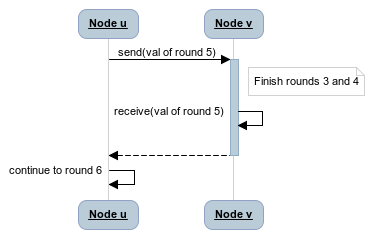
\includegraphics[width=0.5\textwidth]{../figures/sequence1.png}
\label{fig:blocking}}\hfill
\subfloat[Network with non-blocking communication operations]{
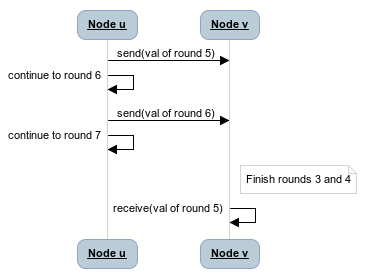
\includegraphics[width=0.4\textwidth]{../figures/sequence2.png}
\label{fig:non-blocking}}

\caption{Both networks execute the decentralized algorithm. In the beginning node $u$ is in round $k=5 $ and node $v$ in round $k=3$}
\label{fig:sending_operation}

\end{figure}

\subsubsection*{Types of failures}

The final assumption we need to make is about the types of failures that can appear in both channels and nodes. Defining the kinds of failures we have to expect will better explain the choices in the parts of the protocol that deal with interaction with other nodes.\\

In our model nodes can fail at any time and without a warning. Even though many networks provide liveness detection mechanisms for proactively notifying participants about possible failures, this is not a function that is always available. For this, and to make the proposed protocol truly portable, we need to assume that such a mechanism is not available by the network and if required, should be provided as part of the protocol. Additionally, we assume that a failing node can at some point in the future recover, without making any further assumptions about its state (it could be in the same state as before the failure or in a new one). As an example, consider a peer-to-peer network, where a node $u$ is briefly disconnected from the Internet while our protocol is running. The other nodes might quickly detect $u$'s failure and proceed to the execution of the protocol's future rounds, while $u$ right after re-connecting might attempt to continue the execution of the protocol, sending outdated messages.\\

Finally, we assume that links can also fail by dropping messages, either due to physical failures or due to congestion. However, we also make the assumption that messages cannot be transformed while transferred in a channel, i.e. the message sent will always be the message received. This final assumption is somehow debatable, in the sense that in real networks messages can arrive at their destination malformed. For instance, there are many security concerns regarding peer-to-peer networks due to the fact that often anonymous users are allowed to join, tampering with transfered messages \cite{chien2003malicious}. While this argument is valid, the time constraints of this project do not allow us to take into account such concerns. However, by designing the protocol in an extensible manner, we allow such matters to be addressed in future work.\\


\section{Design Requirements}

Before designing a protocol for computing spectral network properties in a decentralized manner, it is important to analyze the requirements that such a protocol should satisfy. This will help us to better confine our problem and mark some goals that our solution will need to achieve. There has been a wide analysis of requirements for protocols and decentralized systems \cite{Rose01onthe} \cite{Kendall:1994:NDC:974938}. Those that are the most important in our case, both functional and non-functional, are presented below:


\subsubsection*{Correctness}

The protocol should yield correct results. That is, the exchange of control messages and matrix components should lead to the computation of accurate estimations, which once analyzed should reveal properties of the network that closely resemble its actual properties. There are various ways of verifying the protocol's correctness, from manually checking the intermediate steps performed in multiple protocol runs to comparing the final results that these runs return with the results presented in the algorithm's original evaluation \cite{6195806}.


\subsubsection*{Robustness}

Robustness is a very important requirement of the proposed protocol, since most real-life networks and overlays present topological changes either due to node failures or due to churn. The protocol should be resilient and easily adaptable to such changes. This is translated into a requirement of retaining the algorithm's precision as much as possible regardless of the deployment environment. 

\subsubsection*{Complexity}

With the term complexity we generally refer to a number of parameters which can affect the performance of a system. Those that are important for our protocol are:

\begin{description}
\item[Time Complexity]  The protocol should terminate in as few steps as possible. Since the algorithm by Carzaniga et. al requires exactly $k$ steps to complete, one for each impulse response, we would like our protocol to terminate in at most $\mathcal{O}(k)$ steps, even after the extensions we propose.\\
\item[Space Complexity] The algorithm is expected to be used in large networks composed of hundreds or thousands of nodes, where normally the number of neighbors of each node will be relatively small. As a result, the adjacency matrix and all matrices related to it will be relatively sparse. If these data are not properly stored and managed, the space requirements of the protocol could be really high. The same thing holds for all the information that each node participating in the protocol should store, like lists of neighbors, information about protocol runs, impulse responses etc.\\
\item[Number and Size of Messages] The protocol should send as few messages as possible, in a compact manner such that the size of the messages is minimal. This requirement is particularly important for control messages. As control  messages, we refer to all those messages that are required by the protocol to ensure its proper functionality, but which are not related to the algorithm, e.g a message that checks whether a remote node is alive.  We would like to minimize the use of such messages and if possible to completely integrate them to messages that have a payload useful for the algorithmic operations.\\
\end{description}

\subsubsection*{Termination}

While the termination requirement might seem obvious, it is a very important property that the protocol must hold. It is easy to show that the original algorithm proposed by Carzaniga et al. does terminate in a finite number of rounds, defined by a constant $k$. However when trying to design a concrete implementation of the algorithm, a number of parameters that were previously of no concern could affect the outcome of the protocol's execution. These parameters are mostly related to implementation details and the way certain exceptional situations should be handled. Handling such an exceptional situation in the wrong way could make the protocol block and never terminate. For instance, consider a scenario in which a node $u$ is in round $r$ of the algorithm and waits to collect all the values from its in-neighbors, but one of those neighbors fails. The simple algorithm of Section \ref{sec:decentralized_algo} would assume that $u$ would somehow detect the failure of its neighbor and would not expect to receive a value. However, if such a situation was not handled properly in the concrete implementation (e.g. $u$ never tried to detect failed neighbors), the protocol would never terminate, with $u$ waiting to receive a message which will never arrive.


\subsubsection*{Extensibility}

Even if the proposed protocol achieves its goals, it is possible that unforeseen problems might arise in the future that will need to be solved. Thus, it is important to provide mechanisms that will simplify the addition of functionality or the customization of the protocol's behavior.

\subsubsection*{Efficiency}

A well-designed protocol should be efficient. This means that the choices made for the protocol's mechanisms (etc. how messages will be encoded) should result in a fast and reliable protocol more than anything. However, sometimes efficiency might have to be compromised in order for other properties, like the aforementioned extensibility to be satisfied.

\subsection{Additional Considerations}

Apart from the aforementioned requirements, it is essential to discuss some additional considerations that we will need to have in mind before attempting to sketch a more detailed protocol design. The first is that computing some global properties in the network should mainly be considered as a maintenance routine and not as the main activity of a node. This means that every node in the network might need to use the estimations of the global properties provided by our proposed protocol to perform some actions, but the task of computing those properties will in most  cases not be the main activity of the nodes. Thus performing those computations should be an operation executed concurrently, without blocking the node's main activity.\\

One final consideration is relevant to the fact that  decentralized networks allow nodes to actively join and depart, while failures of nodes are also a possibility. Depending on the underlying network, detecting those topological changes might be a functionality provided by the network itself, although there could also be cases in which they should be detected by the intermediate level of the protocol. In such cases other mechanisms, like failure detectors \cite{Chandra:1996:UFD:226643.226647} might be required to solve the problem.

\section{In-depth Protocol Analysis}

In this section we give a detailed description of our proposed protocol, which can be applied in any network satisfying the assumptions described in Section \ref{sec:model_assumptions}. Additionally, we explain how this protocol can be easily applied in unstable networks affected by failures and/or churn just by properly configuring its execution parameters. 


\subsection{Definitions}

We begin by giving the definitions of the basic structures our protocol is based on:

\begin{description}
  \item[Execution] \hfill \\
  An \textit{Execution} is a part of a protocol run, responsible for completing the tasks described in the original algorithm by Carzaniga et al. in Section \ref{sec:decentralized_algo}. An \textit{Execution} can be divided into three phases; \textit{Initiation}, \textit{Data Exchange} and \textit{Gossip Round}. Each \textit{Execution} holds all the information that are required for the algorithm to run and for the computation of the estimated eigenvalues to be performed. A detailed list of the information maintained by an \textit{Execution} is presented in Table \ref{table:execution_fields}. A completed \textit{Execution}, i.e. with all three aforementioned phases complete, is expected \begin{inparaenum}[\itshape a\upshape)]
  \item to have used the impulse responses gathered to compute a system realization as explained in Section  \ref{sec:decentralized_algo}; 
  \item to have computed the dominant eigenvalues of matrix $A$; and
  \item to have computed the median of the dominant eigenvalues exchanged with the node's neighbors.
  \end{inparaenum}
  An \textit{Execution} also holds an integer value $e \ge 1$, which is used as part of the \textit{Execution}'s full identifier, as explained later. 
  
  \begin{table}
  \centering
	\begin{tabular}{|l|l|}
	\hline
	\multicolumn{2}{|c|}{\textbf{\textit{Execution}}}\\
	\hline
	\hline
	\textit{Execution number e} & Matrix $A$\\
   	\textit{Number of rounds} & Dominant eigenvalues of $A$\\
   	\textit{Current round $k$} & Median of exchanged eigenvalues\\
    \textit{List of in-neighbors} & \\
    \textit{List of out-neighbors} &\\
    \textit{Impulse responses h(t)} &\\
    \textit{Current and future incoming values} &\\
    \hline
  	\end{tabular}
  	\caption{Information stored in an \textit{Execution}. On the right column are the expected results}
  	\label{table:execution_fields}
  \end{table}
  
   \item[Session] \hfill \\
  A \textit{Session} is a full protocol run, containing at least one but possibly multiple overlapping \textit{Executions}. When a user or an application makes a request to the protocol for a sample, a new \textit{Session} is generated by the querying node also known as the \textit{Initiator}, which is spread to all participating nodes. This means that it is possible to have multiple protocol \textit{Sessions} running in the same network simultaneously, generated by queries made in different nodes. Each \textit{Session} has a unique identifier or \textit{SessionId}, distinguishing it from other executions, present and past. The \textit{SessionId}, along with the execution number $e$ is used to provide complete identification of an \textit{Execution} (\textit{Executions} in different \textit{Sessions} can have the same number $e$). A \textit{Session} is considered completed only once all of its \textit{Executions} have terminated. Finally, the \textit{Sessions} stored at each node have an \textit{initiator} flag, dictating whether the local node initiated the present \textit{Session} or not. The reason for this is that the \textit{initiator} node is always responsible for initiating new \textit{Executions} in the context of a \textit{Session}, as it will be explained later. A summary of the information held in a \textit{Session} can be seen it Table \ref{table:session_fields}
   
   \begin{table}
     \centering
   	\begin{tabular}{|l|}
   	\hline
   \textbf{\textit{Session}}\\
   	\hline
   	\hline
   	 \textit{SessionId}\\
     \textit{List of Executions}\\
     \textit{Number of completed Executions}\\
     \textit{Initiator node flag }\\
       \hline
     	\end{tabular}
     	\caption{Information stored in a \textit{Session}}
     	\label{table:session_fields}
     \end{table}
   
\end{description}

\subsection{Protocol Description}
\label{sec:protocol_description}

To better present our proposal, this protocol is analyzed for realizing a system in which matrix $A$ is the uniform transition probability matrix of the network, i.e. position $a_{uv}$ of the matrix is equal to $1/degree(v)$ (remember that information for this protocol are stored \textit{column-wise}).  However, every detail presented in this section applies to any matrix $A$ related to the adjacency matrix, as long as each node can compute its required information locally.\\


The protocol starts running once a sampling request is made by a user or an application to one of the network's nodes. The sampling request contains all the information required for a \textit{Session} to be generated, i.e. the number $m$ of \textit{Executions} and the number $k$ of rounds in each \textit{Execution}. The node that received the sampling request is called the \textit{initiator} and the rest of the nodes are called \textit{participants}.\\


As illustrated in Figure \ref{fig:session_creation_activity}, upon receiving the new request, the \textit{initiator} creates a new \textit{Session} with the parameters provided and sets the \textit{Session}'s \textit{initiator} flag to {\bf true}. An initial \textit{Execution} is also created, with its execution number set to $e=1$. Both the initial and all consecutive \textit{Executions} of the \textit{Session} go through three phases; \textit{Initiation}, \textit{Data Exchange} and \textit{Gossip Round}.

\begin{figure}[h]
\centering
\subfloat[New $Session$ creation activity]{
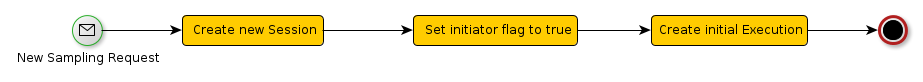
\includegraphics[width=1\textwidth]{../figures/session_creation.png}
\label{fig:session_creation_activity}}\hfill
\subfloat[Contents of a $Session$ right after initialization]{
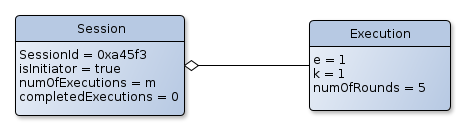
\includegraphics[width=0.6\textwidth]{../figures/session_execution.png}
\label{fig:session_execution}}
\caption{Creation of a new \textit{Session}}
\label{fig:session_creation}
\end{figure}



\subsubsection*{\textit{Initiation}}

The behavior of each node in this phase diverges depending on its role (\textit{initiator} or \textit{participant}). There are certain actions performed only by the \textit{initiator}, while the rest are performed by all nodes.
	
\begin{description}
	\item[Initiator] \hfill \\
	The actions of the \textit{initiator} node $i$ are presented in Task \ref{alg:init_init}:
		\floatname{algorithm}{Task} 
					 \setcounter{algorithm}{0}
					\begin{algorithm}
					\caption{Initiation procedure at node $i$}
					\label{alg:init_init}
					\begin{algorithmic}[1]
					\STATE $x_{i,1} \leftarrow$  Choose a value uniformly from $\{0,1\}$
					\STATE Set $h_i(1)=x_{i,1}$
					\STATE $out\_list \leftarrow$  Get list of \textit{out-neighbors}
					\STATE $weight \leftarrow 1/sizeof(out\_list)$
					\STATE $val \leftarrow x_{i,1}weight $
					\STATE Create an $INIT$ message and add $val$ to it
					\FORALL{$u$ in $out\_list$}
					\STATE Send $INIT$ message to $u$
					\ENDFOR
					\STATE Set $init\_timer$ to initial value
					\end{algorithmic}
					\end{algorithm}	
		
	 The node initially chooses some value $x_{i,1}$ uniformly from the set $\{0,1\}$. This value is also set as the impulse response $h_i(1)$ of round 1. It then gets the list of all its \textit{out-neighbors} from the underlying network. The way this is achieved technically will be explained when presenting the architecture in Section \ref{sec:architecture} and in even more detail in Chapter \ref{sec:implementation}. This list, will be immutable for the \textit{Execution}, until its termination, retaining even failed nodes. This means that once an \textit{Execution} is initiated, a "snapshot" of the network's topology is taken by the node, which does not change through its life-cycle. Even if a new node joins the network in a later round, it will be completely ignored in the context of the particular \textit{Execution}, since it will not be part of its out-neighbors list.
	
	\begin{table}
	\centering
\begin{tabular}{|l|}
		     	   	\hline
		     	   \textbf{\textit{INIT}}\\
		     	   	\hline
		     	   	\hline
		     	   	 \textit{SessionId}\\
		     	     \textit{Total number of Executions}\\
		     	     \textit{Number of new Execution e}\\
		     	     \textit{Total number of rounds k}\\
		     	      \textit{Value} $x_{v,2}$\\
		     	       \hline
		     	   \end{tabular} 
		     	   \caption{Contents of the \textit{INIT} message}
		     	   \label{table:init_msg}
	\end{table}

		     

	Since we want to estimate the uniform transition probability matrix, instead of computing one value $a_{ui}$ for each node $u$, we can simply compute a common weight as shown in line 3, since the probabilities for all nodes $u$ will be the same. If the wanted matrix was different, then the corresponding values should be computed accordingly. 
	
	The next step is to compute the product of $x_{i,1}$ and the $weight$ as defined in the original algorithm and to send this value to all the nodes in the \textit{out-neighbors} list as part of an $INIT$ message. Apart from the value, this message contains all the information required for a node receiving it to create the \textit{Session} and the \textit{Execution}, i.e. the \textit{SessionId}, the execution number $e$ etc. A detailed description of the contents of an $INIT$ message is given at Table \ref{table:init_msg}. Finally an \textit{init\_timer} is set to some globally defined value shared by all the nodes in the network. The value of this timer corresponds to the time left in the \textit{Initiation} phase and is also the time that the node has left to discover its \textit{in-neighbors}.
				
	\item[All nodes] \hfill \\
	The actions described in Task \ref{alg:init_all} are performed by all the nodes in the network, both \textit{initiator} and \textit{participants}:
		\begin{algorithm}
			\caption{Initiation procedure at any node $u$}
			\label{alg:init_all}
			\begin{algorithmic}[1]
			\STATE Upon receipt of an $INIT$ message from node $u$
			\IF{$SessionId$ s does not exist}
			\STATE  Create a new \textit{Session} with id $s$
			\ENDIF
			\IF{$Execution$ $e$ does not exist} 
			\STATE Create a new \textit{Execution} setting its number to $e$
			\STATE Perform the actions described in Task \ref{alg:init_init}
			\ENDIF
			\IF{ $init\_timer$ of \textit{Execution} $e$ has not expired yet}
			\STATE $x_{u,2} \leftarrow x_{u,2}+val$
			\STATE Add $u$ to the \textit{in-list} of $e$
			\ENDIF
			\end{algorithmic}
			\end{algorithm}
	
	 When a node receives an $INIT$ message, it checks whether the \textit{Session} mentioned in the message exists and if not it creates it. The same thing goes for the \textit{Execution}. If the \textit{Execution} did not previously exist, then it should be created as described in Task \ref{alg:init_init}. This means that new $INIT$ messages have to be sent to all the \textit{out-neighbors}, an $init\_timer$ has to be set etc. Finally, in all the cases that the  $init\_timer$ of the \textit{Execution} is still running, the value contained in the $INIT$ message will be added to the values $x_{u,2}$ kept by the \textit{Execution} for round 2 and the node that sent that message will be added to the list of \textit{in-neighbors} of this \textit{Execution}.
	

	
\end{description}


The actions of the \textit{Initiation} phase achieve three things:
\begin{description}
\item[First] They allow all nodes in the network to be informed that a new protocol \textit{Execution} is running. Each node that receives an $INIT$ message, will have a \textit{Session} and an \textit{Execution} with the same id when Task \ref{alg:init_all} terminates. Since each node will send the $INIT$ message to all of its \textit{out-neighbors} and since we have assumed that the graph of the network is strongly connected, we are certain that at some point, all nodes will know about the newly created \textit{Execution}. Also, each node will send an $INIT$ message to its \textit{out-neighbors} for a particular \textit{Execution} only once, that is, when the first $INIT$ message for that \textit{Execution} is received. Thus, the initiation of a new \textit{Execution} is spread to the network nodes using a \textit{controlled flooding} mechanism.
\item[Second] The nodes of the network discover their in-neighbors in the context of the specific \textit{Execution}. One thing that must be noted here is that the proposed method does not guarantee that all in-neighbors will be discovered, since a delay might force an INIT message to arrive after the timer expires. However, a reasonable $init\_timer$ value will allow most of the time the construction of an accurate depiction of the network's actual topology. Additionally, the chances of discovering the actual network topology in a \textit{Session} with more than one \textit{Executions} are increased. Even if the $init\_timer$ of one \textit{Execution} expires before all the \textit{in-neighbors} are located, it is highly likely that the rest of the \textit{Executions} will have better results. Having good results in the majority of \textit{Executions} is enough to get accurate final results, as we shall discuss later in this Section. 
\item[Third] The \textit{impulse response} of round 2 can be computed right after the \textit{Initiation} phase terminates. The reason is that every node that sends an $INIT$ message, appends to it its \textit{impulse} signal for round 2. Thus, the value $x_{u,2}$ used in Task \ref{alg:init_all}, will be the sum of the \textit{impulses} of all the \textit{in-neighbors} of $u$ in round 2, i.e. it will be the \textit{impulse response} of round 2. This is an optimization which reduces the total number of rounds required in the \textit{Data Exchange} phase of the \textit{Execution} by 1.
\end{description}

 
  
\subsubsection*{\textit{Data Exchange}}

Once the $init\_timer$ of an \textit{Execution} terminates, the \textit{Data Exchange} phase begins. This phase consists of a number of rounds $r=3\dots k$. In each round $r$ each node sends an \textit{impulse}, and waits to receive the impulses of the nodes stored in its \textit{in-neighbors} list in order to compute the \textit{impulse response} $h(r)$.\\

\begin{figure} [b]
\centering
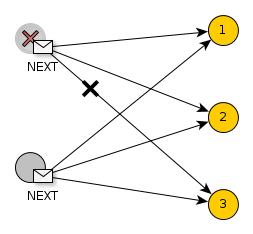
\includegraphics[width=0.3\textwidth]{../figures/partial_network.png}
\caption{Part of a network with a node failing before sending messages for the next round to all its out-neighbors}
\label{fig:partial_network}
\end{figure}

A challenge of this phase is locating in-neighbors which have failed. In the original algorithm a node needs to wait at each round of an execution to receive all incoming messages belonging to this round before proceeding. However, in the case that a node fails before sending all of its messages, its out-neighbors might face a deadlock situation, waiting forever to receive a message that will never arrive. For example, consider the partial network of Figure \ref{fig:partial_network}. All three yellow nodes have an in-neighborhood composed of the 2 gray nodes, so they expect to receive two impulse signals. The gray nodes both send messages containing impulses to the yellow nodes, however the node with the red $X$ fails before sending the message to the third yellow node. Yellow nodes 1 and 2 will proceed without any problem, since they will receive both messages, but node 3 will be permanently blocked waiting the message of the failed node. Such a scenario is avoided in our protocol, as it will be explained in this section, by using a simple failure detection mechanism.\\



\begin{table}
\centering
 \begin{tabular}{|l|}
	     	   	\hline
	     	   \textbf{\textit{NEXT}}\\
	     	   	\hline
	     	   	\hline
	     	   	 \textit{SessionId}\\
	     	     \textit{Number of Execution}\\
	     	     \textit{Number of round}\\
	     	     \textit{Value $x_{v,round}$}\\
	     	       \hline
	   \end{tabular}
	   \caption{Contents of the \textit{NEXT} message}
	   		     	   \label{table:next_msg}
\end{table}



Each round of this phase consists of three tasks. The first actions that a node $u$ performs once a new round is initiated are presented in Task \ref{alg:send_next}: 
\floatname{algorithm}{Task} 
\begin{algorithm}
 		\caption{Initiation of round $r$ of the Data Exchange phase in node $u$}
 		\label{alg:send_next}
 		\begin{algorithmic}[1]
 		\STATE $val \leftarrow h_u(r-1)weight$
 		\STATE Create a $NEXT$ message and add $val$ to it
 		\FORALL{$v$ in $out\_list$}
 		\STATE Send $NEXT$ message to $v$
 		\ENDFOR
 		\FORALL{$i$ in $in\_list$}
 		\STATE $timer(i) \leftarrow$ MAX\_TIME
 		\ENDFOR
 		\end{algorithmic}
 	\end{algorithm}

Initially, the node computes the \textit{impulse}, which should be sent to its \textit{out-neighbors}. The \textit{impulse} of round $r$ is nothing more than the \textit{impulse response} of $u$ in round $r-1$ multiplied by $a_{vu}$, which as in the \textit{Initiation} phase will be $1/sizeof(out\_list)$. Then, $u$ creates a $NEXT$ message containing the computed impulse $val$. This message also contains all the information required by the receiving node in order to add the impulse to the proper \textit{Session}, \textit{Execution} and round. The detailed description of the contents of a $NEXT$ message is given at Table \ref{table:next_msg}. This $NEXT$ message is then sent to all the out-neighbors of $u$, using the list constructed by the \textit{Execution} during the \textit{Initiation} phase. Finally, in each record of the \textit{in-neighbors} list, a field with an $expiry\_time$ is set to a value of MAX\_TIME. This field will be used later to notify the failure detection mechanism that a node should be probed for liveness. \\
 


At this point, the node performs concurrently Tasks \ref{alg:receive_next} and \ref{alg:periodic_task}. Task \ref{alg:receive_next} is executed every time a $NEXT$ message is received:

\begin{algorithm}
 		\caption{Node $u$ receives a $NEXT$ message from node $v$}
 		\label{alg:receive_next}
 		\begin{algorithmic}[1]
		 \STATE $r \leftarrow round\_of(NEXT)$
		 \STATE $val \leftarrow value\_of(NEXT)$
		 \IF{$Execution$ with $SessionId$ $s$ \AND execution number $e$ exists }
		 \STATE $x_{u,r} \leftarrow x_{u,r} + val$
		 \IF{$r$ is current round}
		 \STATE $timer(v) \leftarrow$ INF
		 \ELSE
		 \STATE Add $v$ to $senders\_list(round)$
		 \ENDIF
		 \ENDIF
 		\end{algorithmic}
\end{algorithm}

The node checks whether the \textit{Session} and the \textit{Execution} referenced by the message exist. If they exist, the node adds the value $val$ contained in the message to the values $x_{u,r}$ of round $r$. If they do not exist, the message is completely ignored. Additionally, if the message was intended for the current round, the timer of the sender is set to INF, a special value indicating that an in-neighbor has made contact in the current round. If the message was for a future round, then the id of the sender is stored in a list with all the in-neighbors that have sent a message for that round. \\
\floatname{algorithm}{Task}



Task \ref{alg:periodic_task} is a \textit{periodic} task which runs for each \textit{Execution} and which is responsible for both detecting failures and advancing the protocol to the next round.

\begin{algorithm}
 		\caption{Node $u$ runs the periodic task of the Data Exchange phase in round $r$}
 		\label{alg:periodic_task}
 		\begin{algorithmic}[1]
		 \FORALL{$v$ in $in\_list$}
		 \IF{$timer(v) = 0$}
		 \STATE Probe node $v$ for liveness
		 \IF{$v$ is still alive}
		 \STATE $timer(v) \leftarrow$ MAX\_TIME
		 \ELSE
		 \STATE Remove $v$ from $in\_list$
		 \ENDIF
		 \ENDIF
		 \ENDFOR
		 \IF{all nodes in $in\_list$ have their timer set to INF}
		 \STATE $h_u(r) \leftarrow x_{u,r}$
		 \STATE $r \leftarrow r+1$
		 		 \FORALL{$v$ in $senders\_list(r)$}
		 		 \STATE $timer(v) \leftarrow$ MAX\_TIME
		 		 \ENDFOR
		 \STATE Execute the actions of Task \ref{alg:send_next}
		 \STATE $//$Only in the initial \textit{Execution} of a \textit{Session}
		 \STATE $ratio=num\_of\_rounds/num\_of\_executions$
		 \IF {$u$ is initiator \AND ($r \mod{ratio} =0$) \AND $Session$ has more $Executions$ }
		 \STATE Execute the actions of Task \ref{alg:init_init}
		 \ENDIF
		 \ENDIF
 		\end{algorithmic}
\end{algorithm}

In this task the node first checks all of the nodes in the in-neighbors list of the \textit{Execution} to see if their timers have expired. If the timer of a node $v$ has expired, then that node is probed for liveness. If the node is still alive and replies to the probe, then its timer is renewed, otherwise the node is removed from the list.\\



The node then checks whether all the in-neighbors of the \textit{Execution} have their timers set to INF, in order to proceed to the next round. Since all failed nodes will eventually be removed, at some point all available $NEXT$ messages will be received and the timers of all the live nodes will be set to INF. Thus, the protocol will never block waiting for messages from failed nodes. If the \textit{Exeution} was in round $r$, then the \textit{impulse response} of this round becomes $h_u(r)=x_{u,r}$, since $x_{u,r}$ is the sum of all the values sent by the in-neighbors. The \textit{Execution} then goes to round $r+1$ performing again from the beginning the task described in Task \ref{alg:send_next}, that is, send $NEXT$ messages to out-neighbors and renew the timers of the in-neighbors. It also checks whether any messages were received for the new round during some past round and sets the timer of the sending nodes to INF (lines 14-16).\\

The final step in lines 16-20 is executed only when the initial \textit{Execution} is being checked and if the present node is the \textit{initiator} of the \textit{Session}. This step checks whether a new \textit{Execution} should be initiated in the context of the current \textit{Session}. The ratio computed in line 16, defines the distance, in rounds, of one \textit{Execution} from the next. For example, if we had a Session with 3 Executions of 30 rounds each, the ratio would be 30/3=10, meaning that \textit{Execution} number 2 would be created once the first \textit{Exection} reached round 10 and the third once the first reached round 20. The reason this step is performed only in the initial \textit{Execution} is to avoid creating the same \textit{Execution} multiple times. Otherwise, all the running \textit{Executions} would create new ones in round 10 etc.\\



Once all $k$ rounds of an \textit{Execution} in node $u$ have completed the impulse responses $h_u(1)\dots h_u(k)$ are given as input to Kung's realization algorithm in order to identify matrix $A$ of the dynamic system as explained in Section \ref{sec:kung}. As the final step of the \textit{Data Exchange} phase, the eigenvalues of this matrix are computed and are stored in the \textit{Execution}.






\subsubsection*{\textit{Gossip Round}}

The last phase of the protocol is the \textit{Gossip Round}. This round is very similar to a regular round of the \textit{Data Exchange} phase with the only differences being that instead of impulses, the dominant eigenvalues computed in the end of the previous phase are sent to the out-neighbors and that there are no checks for initiation of new \textit{Executions}.

\begin{table}
	 \centering
	     	     \begin{tabular}{|l|}
	     	     	   	\hline
	     	     	   \textbf{\textit{GOSSIP}}\\
	     	     	   	\hline
	     	     	   	\hline
	     	     	   	 \textit{SessionId}\\
	     	     	     \textit{Number of Execution}\\
	     	     	     \textit{Computed eigenvalues}\\
	     	     	       \hline
	     	     	     	\end{tabular}
\caption{Contents of the \textit{INIT} message}
		     	   \label{table:gossip_msg}
\end{table}	

\noindent The initiation of the \textit{Gossip Round} can be seen in Task \ref{alg:send_gossip}:

\begin{algorithm}
 		\caption{Initiation of \textit{Gossip Round} in node $u$}
 		\label{alg:send_gossip}
 		\begin{algorithmic}[1]
 		\STATE Create a $GOSSIP$ message and add the computed eigenvalues to it
 		\FORALL{$v$ in $out\_list$}
 		\STATE Send $GOSSIP$ message to $v$
 		\ENDFOR
 		\FORALL{$i$ in $in\_list$}
 		\STATE $timer(i) \leftarrow$ MAX\_TIME
 		\ENDFOR
 		\end{algorithmic}
 	\end{algorithm}

This time the node creates a message of type $GOSSIP$ in which the computed eigenvalues are appended. The number of eigenvalues added is not strictly defined by the protocol and setting this parameter should depend on the information we are expecting to receive from the spectral analysis. For example, if we want to compute the \textit{mixing time} of the network, we only need the eigenvalue with the second largest modulus, thus attaching more eigenvalues in the $GOSSIP$ message might be a redundancy. Apart from the eigenvalues, the $GOSSIP$ message used in this phase requires only the $SessionId$ and the execution number $e$ as shown in Table \ref{table:gossip_msg}. Since this phase has only one round, these information are enough for the receiving node to properly handle the message.\\

 

The node sends the $GOSSIP$ message to all of its out-neighbors and sets the timers of all the in-neighbors to a MAX\_TIME value, exactly as in the \textit{Data Exchange} phase. It then runs concurrently Tasks \ref{alg:receive_gossip} and \ref{alg:periodic_task_gossip}. Task \ref{alg:receive_gossip} simply adds the eigenvalues received by any incoming $GOSSIP$ message to a list of proposed values and sets the timer of the sender to INF. 

\begin{algorithm}
 		\caption{Node $u$ receives a $GOSSIP$ message from node $v$}
 		\label{alg:receive_gossip}
 		\begin{algorithmic}[1]
		 \IF{$Execution$ with $SessionId$ $s$ \AND execution number $e$ exists }
		 \STATE Add received eigenvalues to gossip values
		 \STATE $timer(v) \leftarrow$ INF
		 \ENDIF
 		\end{algorithmic}
\end{algorithm}



Finally, Task \ref{alg:periodic_task_gossip} runs periodically checking whether the nodes in the in-neighbors list have sent the expected gossip values or not.

\begin{algorithm}
 		\caption{Node $u$ runs the periodic task of the GOSSIP phase}
 		\label{alg:periodic_task_gossip}
 		\begin{algorithmic}[1]
		 \FORALL{$v$ in $in\_list$}
		 \IF{$timer(v) = 0$}
		 \STATE Probe node $v$ for liveness
		 \IF{$v$ is still alive}
		 \STATE $timer(v) \leftarrow$ MAX\_TIME
		 \ELSE
		 \STATE Remove $v$ from $in\_list$
		 \ENDIF
		 \ENDIF
		 \ENDFOR
		 \IF{all nodes in $in\_list$ have their timer set to INF}
		 \STATE Compute median of proposed eigenvalues
		 \STATE Add \textit{Execution} to list of terminated executions
		 \ENDIF
 		\end{algorithmic}
\end{algorithm}

If the timer of an in-neighbor goes to zero, the node is probed for liveness and if it does not respond, it is removed from the list of in-neighbors. Once all the in-neighbors of the list have their timers set to INF, the gossip phase is over. The final values of the \textit{Execution} are the median of the eigenvalues proposed by the in-neighbors and by the ones computed in the local node. The \textit{Execution} is then appended to a list of terminated executions, stored in the \textit{Session} in which the \textit{Execution} belongs. A \textit{Session} terminates only once the number of \textit{Executions} in this list is equal to the total number of \textit{Executions} $m$, i.e. once all the \textit{Executions} have terminated.



\subsubsection*{Session Termination}

A \textit{Session} terminates only once the number of terminated \textit{Executions} in the context of the \textit{Session} is equal to its total number $m$ of \textit{Executions}. At this point, an estimation of the eigenvalues for the whole \textit{Session} needs to be made.\\ 

Our initial approach in computing the final eigenvalues of the \textit{Session} was to use a simple majority voting scheme, in which the final estimation contains the largest eigenvalues proposed by the majority of \textit{Executions}. However, as we discovered once we ran tests using this approach, such a scheme does not seem to work well and sometimes bad final estimations can be made, even if the majority of the \textit{Executions} propose good estimations. The reason for this is that it is possible for two \textit{Executions} that have made very good estimations to have computed eigenvalues which are slightly different. These differences probably come from the fact that when the protocol is initiated each node chooses as the first impulse either 0 or 1 uniformly at random. Thus, for a network of size $n$, there are $2^n$ initial configurations that the protocol could have, leading into really small differences in the final computed estimations. While these differences are so small that do not affect our results (mixing time etc) they could pose a problem when trying to compute the majority, as two values that we might consider to be equal will actually not be exactly equal. \\

In order to overcome this problem we initially introduced a tolerance value $\epsilon$, so that we could consider two eigenvalues equal even if they had a difference of at most $\epsilon$. In stable networks without the presence of churn, this approach seems to work well, since the differences in accurate estimations are really small. However, when even a single failure is introduced, each \textit{Execution} will propose eigenvalues which are much different than the rest and usually no majority can be found.\\ 

As our final approach, we decided to use the median of all the estimations proposed by all the completed \textit{Executions}. If all the intermediate estimations are accurate, then using this approach we will also give us an accurate final estimation. Even if not all of the estimations are accurate, we still require only the majority, since the median will be part of this majority and thus it will be an accurate estimation. Finally, if all of the estimations are inaccurate, we will at least not end up with an "extreme" estimation, which has a high probability of being very inaccurate.




\subsubsection*{Fault tolerance and Churn}

As explained in the evaluation of the original algorithm by Carzaniga et al. in Section \ref{sec:decentralized_algo}, one problem of the original algorithm is that it's results in the presence of churn or even a single node failure can be very bad. More specifically, the algorithm seems to have a very high percent error when a failure or any topological change occurs in any round $r \ge k/2$. If the number of rounds used is relatively large (e.g. $k=60$) and the failure occurs early on, then the algorithm converges and ultimately returns good results.\\

\begin{figure}[h]
\centering
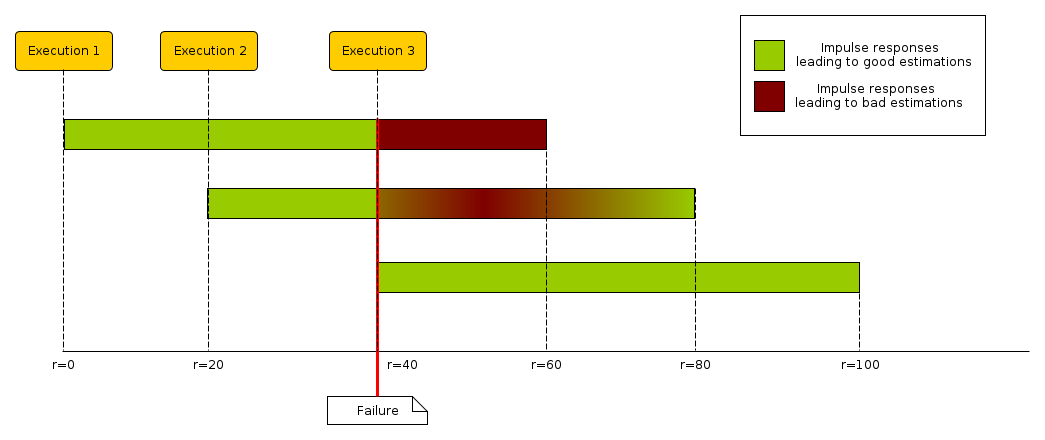
\includegraphics[width=1\textwidth]{../figures/fault_tolerance.png}
\caption{Diagram presenting all the rounds and impulse responses of a \textit{Session}.}
\label{fig:fault_tolerance}
\end{figure}
One very important feature that the proposed protocol offers is its higher tolerance in churn and node failures, compared to the original algorithm, with the use of multiple \textit{Executions} for each sampling request. As explained in the \textit{Data Exchange} phase, the \textit{Executions} of a \textit{Session} are uniformly spaced in time. i.e any \textit{Execution} $e$ will have the same distance $d$ in number of rounds from \textit{Execution} $e-1$. Since failures have negative effects to the estimated results only if they occur in later rounds of an \textit{Execution}, having multiple overlapping \textit{Executions} could lead to a more accurate estimation. For instance, consider a \textit{Session} with 3 \textit{Executions} as illustrated in Figure \ref{fig:fault_tolerance}. The total number of rounds for each \textit{Execution} is 60, thus the total number of rounds in the \textit{Session} because of the pipelining will be 100. If a failure occurs in round $r=40$, \textit{Execution} 1 will already have passed half its rounds and thus it will give a bad estimation. \textit{Execution} 2 will be affected by the failure, however, since this will happen during its $20^{th}$ round it will have plenty of time to recover. Finally, \textit{Execution} 3 will be completely unaffected, since it will be initiated right when the failure occurs. Since 2 out of 3 \textit{Executions} are unaffected, using the median computation scheme previously described will result in the \textit{Session} having accurate results, obliterating the bad estimations due to the failure. \\


Obviously, the effectiveness of this mechanism, greatly depends on the parameters we set for the number of rounds and \textit{Executions}. However, it also depends on the characteristics of the underlying network. For instance, if the network has a high churn rate or a lot of failures occurring frequently, then no \textit{Execution} would be unaffected by the network changes and thus, all estimations would be inaccurate. The magnitude of the error will be defined by the rounds in which the failures will occur.   

\chapter{Software Architecture}
\label{sec:architecture}

This chapter discusses the architecture of our implemented software and presents its constituent components. A lot of the decisions presented in this chapter were made by taking into account the concepts and frequently used technologies presented in Chapter \ref{sec:background} as well as the requirements that we defined in Chapter \ref{sec:design}. This is a high overview of the software, so some inaccuracies and inconsistencies exist in order to keep things simple and to provide a better introduction for the reader. For instance, some parts of the system, like important data structures and detailed descriptions of the components' classes will not be presented here. The actual implementation details of all the software's components will be discussed in depth in Chapter \ref{sec:implementation}.

\section{General overview}

One of the most fundamental challenges that our implementation should address is the protocol's portability into a wide range of different network types with as few modifications as possible. In other words, we desire our implementation to be network-agnostic, making the protocol in a high degree independent from the structure of the underlying network while still retaining all its functionality. \\


Before presenting our proposed approach for providing a network-agnostic service it would be beneficial to briefly discuss the information our protocol requires from the underlying network in order to properly operate and whose acquisition might prove to be challenging due to the distinctive features different types of networks possess.\\

The first requirement for the protocol to properly function is communication with the in and out-neighbors of all the participating nodes. One problem that arises, is that neighbors can be defined differently depending on the network as we have already seen in Chapter \ref{sec:background}.
For instance, as illustrated in Figure \ref{fig:different_neighbors}, in a physical network a neighbor of a node $u$ is considered any other node which directly communicates with $u$. On the other hand, in an overlay network a neighbor of $u$ might be a node physically located several hops away, which has a virtual link to $u$ set according to the rules of the overlay. Additionally, even overlay networks can have completely different definitions for neighboring nodes. For instance, when we analyzed how Chord and Pastry nodes are organized and how routing of messages works in both overlays, we saw that a Chord node would have an immediate communication with the nodes in its \textit{finger table} and its \textit{successor}, while a Pastry node with those in its \textit{leaf set} and the \textit{routing table}.\\

\begin{figure}
\centering
\subfloat[Physical Network]{
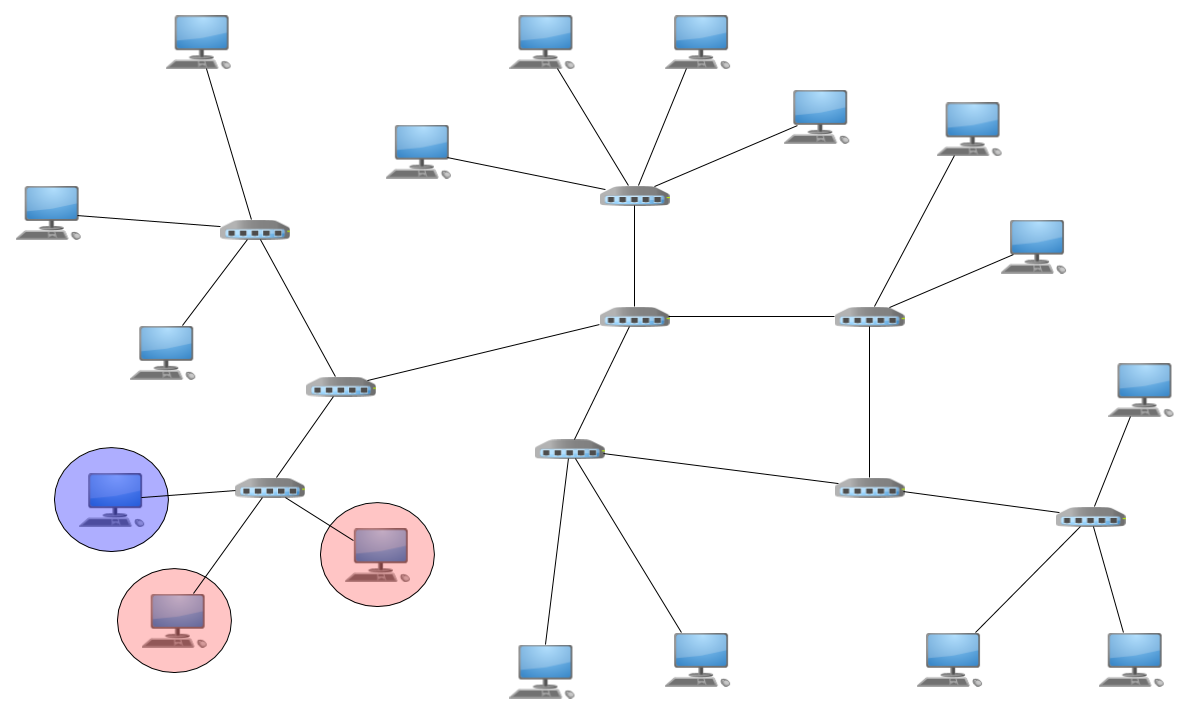
\includegraphics[width=0.45\textwidth]{../figures/physical_neighbors.png}
\label{fig:physical_neighbors}
}\hfill
\subfloat[Overlay Network]{
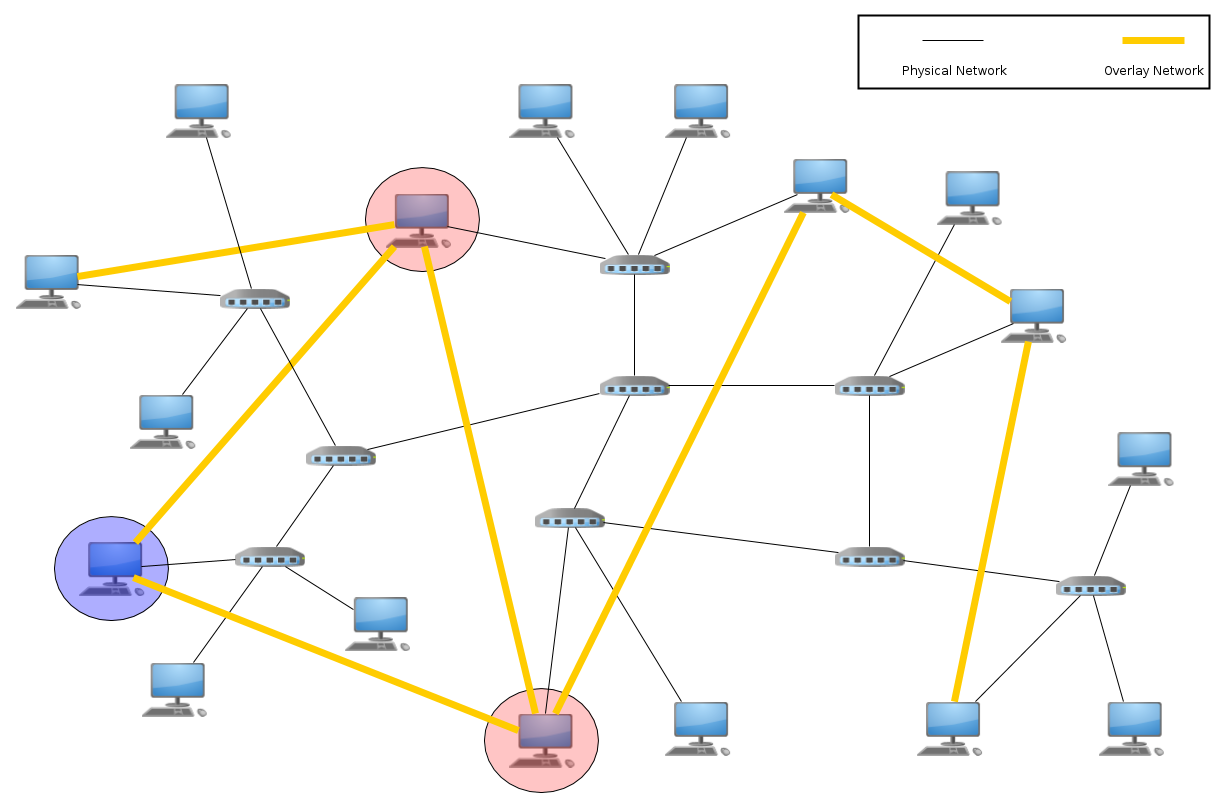
\includegraphics[width=0.45\textwidth]{../figures/overlay_neighbors.png}
\label{fig:overlay_neighbors}
}
\caption{Example of neighboring nodes in physical and overlay networks. The nodes in pink are neighbors of the node in blue. The physical network is in both cases the same.}
\label{fig:different_neighbors}
\end{figure}


The second requirement of the protocol related to the underlying network, which at first glance might not even appear to be a source of trouble, is a way to reference nodes in a unique manner. Every network uses some kind of mechanism for uniquely identifying participating nodes. For instance, in a physical network each node is assigned a unique MAC address distinguishing it from the rest; in a Chord network every node is assigned an $m$-bit identifier after hashing some information with the $SHA-1$ algorithm and in Pastry each node is identified by an 128-bit unsigned integer. It would be ideal for our protocol not to make specific use of any of the aforementioned identification mechanisms for referencing nodes while performing its internal operations, as such an approach would severely restrict the protocol's portability. Instead a more generic referencing mechanism should be used, with its generated references being translated into specific network related ids at a lower level, as Figure \ref{fig:id_mechanism} illustrates. By using such an approach, the network could operate in the same manner for all supporting networks without having to worry about technical details and semantic differences.\\ 


\begin{figure}[h]
\centering
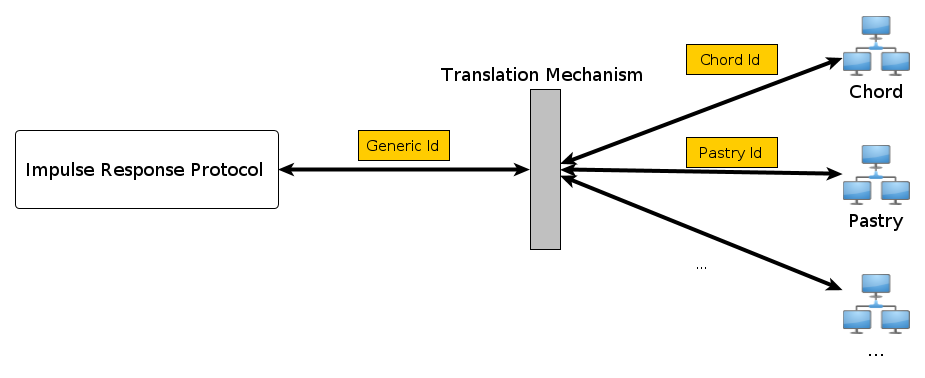
\includegraphics[width=0.9\textwidth]{../figures/id_mechanism.png}
\caption{Id abstraction generic mechanism}
\label{fig:id_mechanism}
\end{figure}


Both the aforementioned requirements demonstrate clearly the need for introducing some kind of abstraction mechanism, which will separate the operations performed as part of the core protocol (i.e. computation of impulse responses, estimation of eigenvalues etc.) from those requiring interaction with the underlying network (i.e. find out-neighbors, find the id of a node etc.). The solution for such a problem is well known and widely applied in networks, through the use of abstraction layers. Perhaps the most well-known example of a layered network architecture is the OSI model \cite{citeulike:915718} used in communication networks to separate the communication operations performed in a node into logical layers, where each layer is responsible for a particular set of operations, independently of how operations in lower layers are implemented. Then for example, operations related to the transport of packets to remote nodes are always performed in the same way, regardless of how nodes are interconnected in the physical level. \\

Using a similar approach our protocol is designed to perform its operations in distinct layers. In Figure \ref{fig:design_overview} we can see the communication stack of a network in which our protocol could be deployed. The base of the stack is the physical network, which we assume to be a network using the IP protocol. While such an assumption is not always valid, the IP protocol is used for communication in the overwhelming majority of real-life networks, both physical and overlays, and thus the choice of developing our protocol on top of IP was made in order to offer better optimizations regarding the mechanisms related to communications (sending messages etc). \\  

\begin{figure}[h]
   \centering
     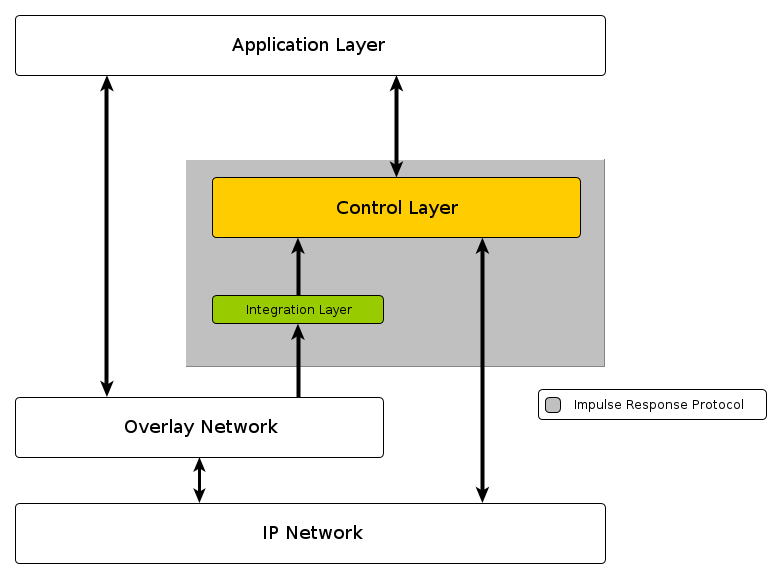
\includegraphics[scale=0.5]{../figures/protocol_stack.png}
	 \caption{Impulse response protocol layered architecture}
     \label{fig:design_overview}
\end{figure}

The second layer in this stack is the overlay network. In this layer we could have any overlay network that could be used on top of IP, e.g. Pastry. The sole assumption that we make for this layer is that in order for an overlay to be supported, it must offer some kind of unique identification for the participating nodes. This is a requirement, which to our knowledge is satisfied by any existing overlay network. The double-sided arrow connecting this layer to the IP layer means that information between the two layers flow unidirectional and it is unrelated to the dependencies of each layer. More specifically, the arrow designates that the overlay uses the IP protocol to both send and receive messages.\\

 
The impulse response protocol implementation is composed of the components in the gray area. We can distinguish two layers; the protocol control layer and the integration layer.


\begin{description}
\item[Control Layer] \hfill \\
 This is the top layer, in which lies the core functionality of our protocol. This layer is responsible for computing impulse responses, managing the protocol's messages ($INIT$, $NEXT$ and $GOSSIP$), estimating matrix $A$ of the surrogate system, computing its eigenvalues etc. It also provides its own generic identification mechanism for referencing remote nodes.

\item[Integration Layer] \hfill \\
 This is the bottom layer of the protocol, which acts as an intermediate between the protocol's control layer and the underlying network. It is responsible for providing the top layer with all the information, which require interaction with the underlying network in order to be obtained. More specifically, this layer provides a mechanism for converting specific network ids to a generic form and a mechanism for obtaining the out-neighbors of the node. The figure shows that this integration layer is connected to the overlay network using a single-sided arrow. This means that this layer does not exchange information with the overlay network, rather pulls any information required once requested by the control layer.
\end{description}

As we can see the protocol control layer communicates with both the integration layer and the IP network, completely overriding the overlay network. As previously mentioned communication with the integration layer is required in order to receive important information regarding the underlying network. On the other hand, the communication of this layer directly to the IP network is required for exchanging information, i.e. sending and receiving protocol-related messages. Communicating with the overlay network, would mean that the impulse response protocol shares traffic with the overlay protocol (i.e. its messages "piggyback" messages of that protocol). While such a design choice might actually allow better performance since no new messages are sent by our protocol, it would also greatly reduce the protocol's portability. "Piggybacking" is also a network-specific operation, different in every overlay, which unfortunately cannot be supported by the integration layer, since not all overlay networks could support it. However, since such a service might improve the protocol's performance it would be interesting to investigate it in some future work.\\

The final layer of the stack is the application layer, in which the application utilizing the overlay network operates. As we can see from Figure \ref{fig:design_overview}, this layer communicates with both the impulse response protocol and the overlay network, which means that from the point of view of the application, the protocol runs in parallel to the operations of the overlay network or as we could say, the overlay network provides the impulse response protocol as an integrated service. While from an architectural point of view this is not accurate, one of the basic ideas of this project is exactly this; anyone who is developing software implementing an overlay network protocol and wishes to gather sampling data, can do so by integrating such a functionality through our proposed software by simply extending it to add support for that specific overlay. More details on how such functionality could be provided in a simple manner will be discussed later in this and the following chapter.



\section{Components}

In this section we give an overview of the components composing each one of the layers presented in the previous section and briefly discuss their interaction. These components do not correspond to software packages or classes in a precise manner, rather they are a logical abstraction created for better explaining things. In reality, some of these components are composed by more than one packages with multiple classes each, while others correspond directly to the actual implementation. These details will be further analyzed in the following chapter, where the implementation of specific classes and their interaction will be presented.

\subsubsection*{Integration Layer}

As discussed earlier, the integration layer exists to provide the impulse response protocol with portability, allowing it to be deployed over any network which fulfills the minimal requirements of providing unique node identification and a list of the node's out-neighbors, regardless of how these neighbors are defined by the overlay. In order to achieve portability, the protocol is designed in a way which allows it to be pluggable. \\

The idea is to further divide the integration layer into two major components or "sub-layers" as illustrated in Figure \ref{fig:integration_layer}. The top sub-layer is composed by a single component which provides the generic interface with which the control layer interacts. Any network-related information is addressed by the control layer in an abstract manner, i.e. there is an abstract way of storing and handling ids and neighbors. Whenever the protocol requires network information it only needs to make a request to the top sub-layer and receive them in the abstract representation it recognizes, without worrying about specific network details. \\

On the other hand, the bottom sub-layer is composed by multiple components, which provide the actual implementation details required for a specific network type. This means that this sub-layer will contain as many components as the number of network types supported by the protocol. These components are responsible for gathering and transforming the data required by the protocol from their concrete representation to their abstract form and to feed them to the top sub-layer, which will in turn make them available to the protocol services.\\

Using the proposed approach greatly increases the protocol's portability as it allows the support of new networks with minimal effort. The only thing that one has to do is to implement methods in the bottom sub-layer of the integration layer, which conform with the abstract interface defined. As it will be shown in Chapter \ref{sec:implementation}, implementing such a component usually requires writing less than 100 lines of code, as long as the API provided by the underlying network allows easy access to the required information (list of neighbors and id of node).


\begin{figure}[]
   \centering
     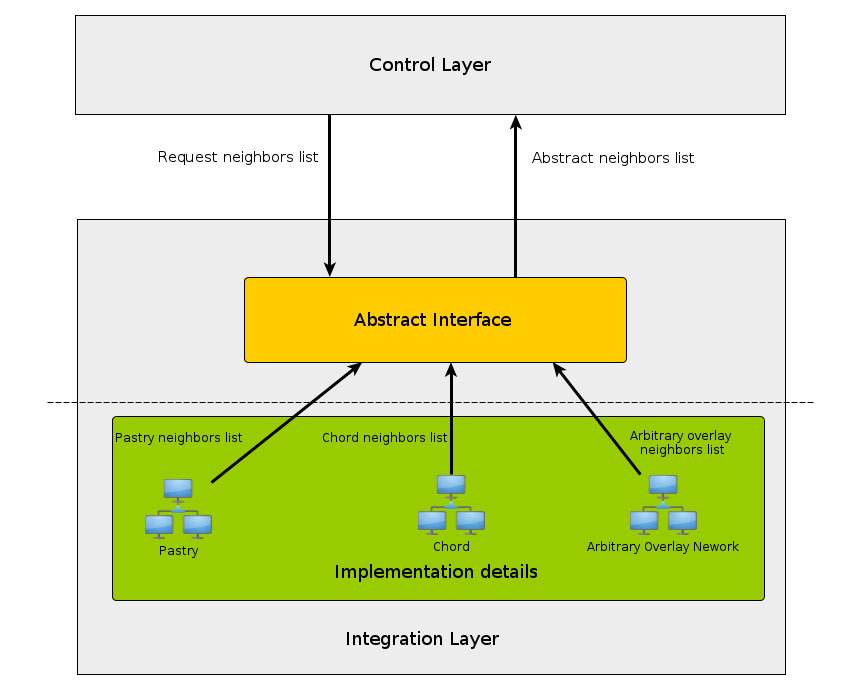
\includegraphics[scale=0.4]{../figures/integration_layer.png}
	 \caption{Interactions in the integration layer}
     \label{fig:integration_layer}
\end{figure}



\subsubsection*{Control Layer}

The top layer of the impulse response protocol is the one that provides the actual protocol service and is composed from the following components, illustrated in Figure \ref{fig:network_agnostic_layer}:

\begin{description}
\item[Protocol Core] \hfill \\
 This is the main software component and is responsible for properly executing the protocol. It also is the most complex component of all, due to the number of actions it performs. First of all, it is responsible for creating and coordinating the various \textit{Sessions} and \textit{Executions} of the protocol, making decisions about the phase they are in, when to advance to the next round, whether they should terminate etc. Additionally, it handles the incoming messages, deciding which value should be added to which \textit{Execution} and whether a new message containing a recently computed value should be sent to the node's out-neighbors. Moreover it is responsible for the protocol's maintenance tasks, like discovering the node's in-neighbors, maintaining the neighbors lists and deciding whether a neighboring node should be probed for liveness. Finally, it provides a simple API, which allows users and applications to make new sampling requests with ease. 
\item[Communications] \hfill \\
The responsibilities of this component are related to the interaction of the protocol with the IP network for sending and receiving messages. As discussed in the previous section, the protocol does not share traffic with the overlay network for portability reasons, which essentially means that any protocol-related messages need to be sent to the remote nodes by direct communication through the IP network. The messages manipulated by this component can be distinguished into two general types, those carrying values and those sent for maintenance tasks. In the first category belong all the messages which carry some value useful for one of the protocol's rounds, i.e. an impulse response-related value for \textit{Initiation} and \textit{Data Exchange} phases or a list of  proposed eigenvalues for the \textit{Gossip} phase. In the second category belong the control messages, sent by the protocol, when probing a node for liveness.\\
\item[Storage] \hfill \\
This component is responsible for storing and retrieving all completed \textit{Sessions} and \textit{Executions}. There are two main reasons for integrating this component to the rest of the software. The first is that we would like to be able to analyze previous network samples which could give us useful information regarding the state of the network. For instance, observing the changes in the network's spectral properties could provide us information about the dynamic evolution of the network \cite{kunegis2007spectral}. The second reason is that the protocol could use the stored information for providing optimizations related to the frequency of taking samples. The basic idea is that if we check the values of previous samples and they are unchanged for a long time, then it is highly likely that we have a stable network, which would require sampling less often. On the other hand, frequent changes in the stored information could be translated in a network with continuous topological changes, requiring samples to be taken in shorter periods of time. This optimization will be presented and explained in depth in the following chapter.
\item[Algorithms and Analysis] \hfill \\
This component is responsible for performing all the algorithmic operations required by the protocol. More specifically, it provides the implementation of Kung's realization algorithm and algorithms for computing and sorting the eigenvalues of matrix $A$ (of the surrogate dynamic system) by the magnitude of their moduli. Additionally, it provides methods for analyzing the estimated eigenvalues after a sampling is complete, e.g. computing mixing time, spectral gap etc. Any new algorithm implemented for the purpose of analyzing the sampling results should also be part of this component.

\end{description}

\begin{figure}
   \centering
     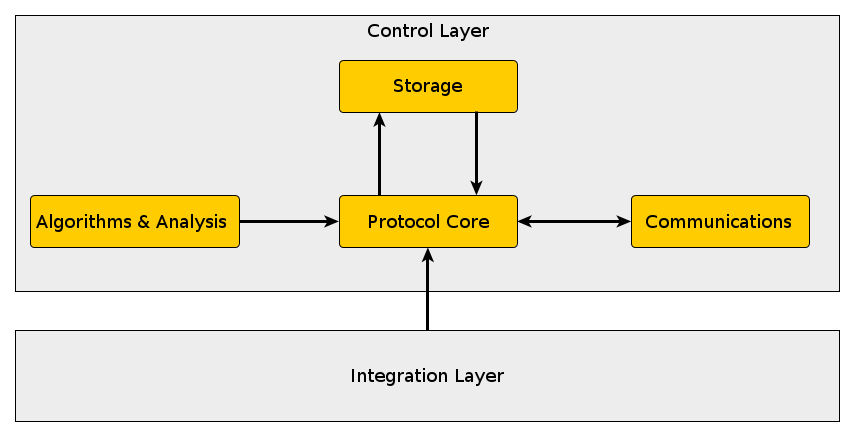
\includegraphics[scale=0.4]{../figures/network_agnostic.png}
	 \caption{Interactions in the control layer}
     \label{fig:network_agnostic_layer}
\end{figure}


\chapter{Implementation}
\label{sec:implementation}

In this chapter we discuss the implementation of each of the impulse response protocol components. Additionally, we present an evaluator component which was created in order to evaluate the results and performance of our software.

\section{Protocol Components}

In this section we discuss the implementation details of the components presented in Chapter \ref{sec:architecture}. Most of the aforementioned components were implemented using the Java programming language, apart from certain mechanisms related to the generation of protocol messages. The points where Java was not used will be highlighted and further explanations of our approach will be provided.

\subsection{Basic Domain Classes and Data Structures}
\label{sec:basic_domain}

Before discussing the implementation of each individual component, we need to present the basic domain classes and data structures used by the protocol. The domain classes used cover three very important issues of the protocol:


\begin{enumerate}
  \item How nodes are identified in the protocol
  \item How the neighbors of a node are internally represented
  \item How the protocol related information (\textit{Executions}, \textit{impulse responses}, rounds etc) are managed internally.
\end{enumerate}

The data structures used are responsible for managing a node's neighbors in an efficient and extensible manner. 


\subsubsection*{Identification Mechanism}

As discussed in the previous chapter, one of the challenges for making the protocol portable is to provide a mechanism for unique identification of the participating nodes. A challenging aspect we faced at this point was that while all types of networks provide some sort of unique node identification, the representation used can vary, i.e. in a physical network the ids are MAC addresses, in a Pastry overlay they are 128-bit unsigned integers, in Chord the ids are produced using the SHA-1 hash function etc.\\

Using the identification mechanism provided by one of these networks would seriously restrict the protocol's applicability to other network types. For instance, let us say that we decided to use IP addresses to reference nodes, since even overlays run on top of the IP network and it is a more generic reference mechanism. In a simple IP network this approach would work well, however, in a network like Pastry, where more than one virtual nodes might run in the same physical machine, the referencing would no longer be unique (both would have the same IP). If on the other hand, we chose to use the identification mechanism of one of the overlays, e.g. Pastry, then our protocol would not be easily portable to other networks like Chord, since we would also need a translation mechanism to map the protocol ids to the Chord ids. Such a mechanism would incur some overhead both in space (to store the translation map) and in time (to look at the map every time we need to contact some node).\\

To tackle this problem, we decided to follow a more generic approach. Any type of data is in reality a collection of bytes, decoded and/or translated in various ways. For instance, in Java, each character of a \classname{String} is represented using two bytes, an integer using 4 bytes etc. This means, that any type of id used by the underlying network can always be represented as an array of bytes. This also means that as long as the ids used by the underlying network are unique, their byte representation will also be unique. For our protocol, we created a  simple wrapper class, called \classname{Id}, which encapsulates the id representation used by any type of underlying network, by simply taking that id and converting it to a byte array. Responsible for converting an id to a byte array is the \textit{Integration Layer} and some examples of conversions will be presented when analyzing that component. \\ 

The ids of our protocol will have varying size, depending on the size of the ids used by the underlying network. For instance when the protocol is deployed on top of Pastry, the ids will be 128-bits long, while in Chord they will be $m$-bits long. The ids can also be easily compared byte-by-byte as shown in Listing \ref{lst:id_comparison}. The big advantage of this approach is that the ids are always provided by the underlying network, while at the same time the control layer of the protocol can reference them in a unique manner through the \classname{Id} class.\\


\begin{lstlisting} [caption=Comparison of ids, label={lst:id_comparison}]
public boolean equals(Id anotherId) {
	// We only need to compare the byte representations of the ids
	return Arrays.equals(this.id.getByteRepresentation(), 
		anotherId.getByteRepresentation());
}
\end{lstlisting}

The final problem of this approach is that even though the byte arrays are practical for internal comparisons while the protocol runs, they are completely impractical when we require a string representation of the ids for verbose execution of the protocol, i.e. for logs etc. Since the binary data of the id are not actual characters, we cannot do a direct conversion to a string. Moreover, presenting the byte array as a hex string could work in cases that the ids are not too long, however since the protocol might be used by various networks with ids of unknown size, we wish to decrease the length of the produced string as much as possible. The way to overcome this problem is by using \textit{Base64} encoding. \textit{Base64} is a binary-to-text encoding scheme, which allows us to represent binary data in an ASCII string format by translating it into a base-64 representation \cite{rfc4648}. This encoding creates strings of smaller length than a hex string, since 4 characters are required for every three bytes, while in hex strings two characters are required for each byte. The results of this conversion is that we get a readable \classname{String} of relatively small length. The different representations of ids using this method can be seen in Table \ref{table:id_representations}.

\begin{table}[bp]
\centering

\begin{tabular}{c |c|}

\cline{2-2}
& \multicolumn{1}{c |}{\textbf{\textit{Pastry Node Id}}} \\
\hline

\multicolumn{1}{|c |}{\textbf{\textit{Original representation}}} & 49940BB1CD20217AA93C5116CCC5A0C9DC94B90B \\
\hline
\multicolumn{1}{|c |}{\textbf{\textit{Id wrapper - Base64}}} & C7mU3MmgxcwWUTypeiEgzbELlEk= \\
\hline
\end{tabular}
\caption{Representation of Pastry ids in their original form (hex) and through the \classname{Id} wrapper }
\label{table:id_representations}
\end{table}

\subsubsection*{Nodes representation and management}

One of the most fundamental elements of the protocol's domain model are the neighbors of each participating node. As a brief reminder, we distinguish the neighbors of a node into \textit{in-neighbors} and \textit{out-neighbors}. In each round $r$ of an \textit{Execution} a node $v$ sends to all of its out-neighbors $u$ the value of the impulse response of the previous round $h_v(r-1)$ multiplied by the element $a_{uv}$ of matrix $A$ and then waits to receive the corresponding values from all of its in-neighbors.  \\

In our implementation, we represent the neighbors of a node by defining a \classname{Neighbor} class. Every \classname{Neighbor} has a unique id of the type \classname{Id} previously described. Additionally, it stores an \classname{InetAddress}, which is used for contacting the node when exchange of information is required by the protocol, i.e. sending messages for some protocol phase or probing a node for liveness. The \classname{Neighbor} class does not store any additional overlay-related information about the remote node, since as explained in Chapter \ref{sec:architecture}, the protocol does not share traffic with the underlying network(i.e. "piggybacking"), rather than uses directly the IP network for its message exchanges.\\

Even though all neighbors share the common features previously described (\classname{Id} and \classname{InetAddress}), they also have certain properties distinguishing them. Each one of the out-neighbors is related to an element of matrix $A$, i.e. element $a_{uv}$ for out-neighbor $u$ of node $v$, where the set of all these elements, constitute the column $A_{v}$ of matrix $A$, stored locally in node $v$. On the other hand, every in-neighbor needs to have a timer, which is required for ensuring that it is alive in the case the local node has not received an expected value from it for a very long time.\\

To handle these differences, the \classname{Neighbor} class was extended by two sub-classes, \classname{PlainNeighbor} and \classname{TimedNeighbor}, as Figure \ref{fig:neighbors_hier} illustrates. A \classname{PlainNeighbor} represents out-neighbors by having an additional \textit{matrixElement} field for storing the proper value of matrix $A$, while a \classname{TimedNeighbor} represents in-neighbors by having a \textit{remainingTime} field. This field will be initialized to a maximum value once the neighbor is created and every time the maintenance task of the protocol executes, the elapsed time since the last check will be subtracted. Once the value of this field gets to 0, the remote node will be pinged to ensure it is alive. Each time a round is complete, the remaining time will be set back to the maximum value. \\

At this point it must be noted, that the \textit{remainingTime} field is not an accurate timer and more precise mechanisms are provided by Java (e.g. \classname{Timer} class). However, there are two main reasons for following this approach. The first is that in most large networks a node is expected to have several in-neighbors. If a timer running in a separate thread was used for each one of them, then the overhead of maintaining and handling this amount of timers would be much higher than just reducing a value whenever a scheduled task ran. The second reason is that we are not that interested in accurately storing the remaining time for each in-neighbor. The only reason that this timer exists in the first place is to avoid deadlocks due to node failures. Our method ensures that a node that is not alive will eventually be probed, even if this happens with a delay of a few milliseconds.\\


\begin{figure} 
   \centering
     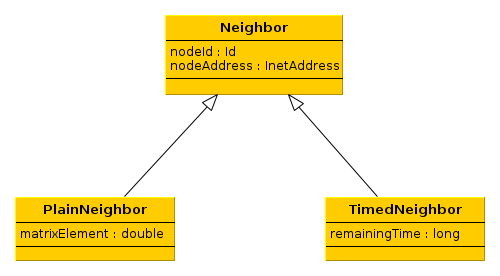
\includegraphics[scale=0.5]{../figures/neighbors.png}
	 \caption{\classname{Neighbor} hierarchy}
     \label{fig:neighbors_hier}
\end{figure}


A final requirement regarding the in and out-neighbors of nodes is that they need to be stored and managed efficiently, so that they do not become a reason for slow protocol responses, due to inefficient neighbor lookups. The approach followed was similar to that of the neighbors themselves as illustrated in Figure \ref{fig:neighbors_tables}. A \classname{NeighborsTable} interface was created, which defines the basic methods that any table maintaining neighbors should implement, i.e. addition and removal of neighbors. This interface was then extended by two additional interfaces, \classname{PlainNeighborsTable} and \classname{TimedNeighborsTable}, one for each of the aforementioned types of neighbors adding additional definitions for management of matrix elements and timers respectively. \\

\begin{figure}
   \centering
     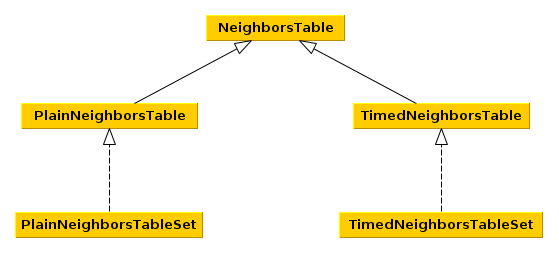
\includegraphics[scale=0.5]{../figures/neighbors_table.png}
	 \caption{\classname{NeighborTable} hierarchy}
     \label{fig:neighbors_tables}
\end{figure}

The reason that \classname{PlainNeighborsTable} and \classname{TimedNeighborsTable} were defined as interfaces and not as concrete classes was to comply with the requirement of extensibility. Using this approach, any developer using the protocol library can easily implement these interfaces using data structures that better suit the needs of a particular network. For instance, networks in which nodes have a large number of in and out-neighbors might require a different data structure from a network where each node has only 2 or 3 neighbors, which can probably be managed effectively using a much simpler and faster data structure.\\

For this project, the implementations provided are \classname{PlainNeighborsTableSet} for the out-neighbors  and \classname{TimedNeighborsTableSet} for the in-neighbors . Both of these classes use the \classname{HashSet<>} class of the \textit{java.util} package. All the operations in these tables have been made thread-safe by using the \textit{synchronizedSet()} method of the \classname{java.util.Collections} class to the underlying hash sets as displayed in Listing \ref{lst:synchronized_tables}. A final notice is that while any actions performed directly over the  
\classname{PlainNeighborsTableSet} and \classname{TimedNeighborsTableSet} tables are thread-safe, synchronization should be done manually when iterating over them.\\

\begin{lstlisting} [caption=Thread-safe PlainNeighborsTableSet with the use of synchronizedSet()., label={lst:synchronized_tables}]
private Set<PlainNeighbor> neighborsList;

//The constructor creates a thread-safe set to store the neighbors	
public PlainNeighborsTableSet() {
	neighborsList = Collections.synchronizedSet(new HashSet<PlainNeighbor>());
}
\end{lstlisting}


\subsubsection*{Representation of protocol related information}

The final part of the protocol's domain model is related to the information concerning the core of the protocol's operation, i.e. management of impulse responses, progress in rounds of execution etc. As discussed in Chapter \ref{sec:design}, the protocol uses two basic structures for these operations, namely a \textit{Session} and an \textit{Execution}. An \textit{Execution} is a part of a protocol run, responsible for completing the tasks described in the original algorithm by Carzaniga et al., while  a \textit{Session} is a full protocol run, containing at least one but possibly multiple overlapping \textit{Executions}. These structures were directly ported into concrete classes using the same names.

\begin{description}
\item[\classname{Execution}] \hfill \\\\
The \classname{Execution} class stores all the information required for one simple execution of the impulse response algorithm (impulse responses, number of current round etc), as well as its computed results, i.e. the realization of matrix $A$ and the computed eigenvalues. An \textit{enum} of type \classname{Phase} (Listing \ref{lst:phases_values}), defines the phase in which an execution is at any point. Setting this phase, is not managed directly by the \classname{Execution} class, rather from a periodically executing maintenance task. This means that the \classname{Execution} does not actively change the phase it is currently in, but this has to be done externally when certain events occur, e.g. the timer of the \textit{Initialization} phase expires etc. This matter will be discussed in further details in Section \ref{sec:protocol_core}, once the protocol's tasks have been presented.


\begin{lstlisting} [caption=Values of the \classname{Phase} enum, label={lst:phases_values}]
public enum Phase {
	INIT, 
	DATA_EXCHANGE, 
	GOSSIP,
	TERMINATED
}
\end{lstlisting}


Additionally, an \classname{Execution} encapsulates a data structure called \classname{GossipData}, in which all the eigenvalues proposed by the in-neighbors of a node are stored during the \textit{Gossip Round} and the median of their moduli is computed. A detail that should be noted at this point, is that there are some cases, where the vectors of the eigenvalues proposed by different neighbors have different sizes, due to the nodes realizing systems of a different order. The reason of why such a thing could happen will be better explained in Section \ref{sec:algorithms} (Algorithms and Analysis). In such cases, only the median of the $k$ largest eigenvalues is computed, where $k$ is the size of the shortest proposed vector of eigenvalues, as in the example shown in Table \ref{table:largest_eigenvalues}. \\


\begin{table}[H]
\centering
\begin{tabular}{c|c|c|c|c|}

\cline{2-5}
& $1^{st}$ eigenvalue & $2^{nd}$ eigenvalue & $3^{rd}$ eigenvalue & $4^{th}$ eigenvalue \\ \hline
\multicolumn{1}{|c|}{$1^{st}$ Proposal} & 0.9856 & 0.7456 & 0.4567 & 0.2178\\
\hline
\multicolumn{1}{|c|}{$2^{nd}$ Proposal} & 0.9882 & 0.7362 & 0.4567 & \cellcolor{lightgray}\\
\hline
\multicolumn{1}{|c|}{$3^{rd}$ Proposal} & 0.9856 & 0.7456 & 0.4278 & 0.2178 \\
\hline
\hline
\multicolumn{1}{|c|}{Median} & 0.9856 & 0.7456 & 0.4567 & \cellcolor{lightgray} \\
\hline

\end{tabular}
\caption{Eigenvalue proposals of different sizes made by 3 nodes and their median. Only the three largest eigenvalues will be computed, since the second proposal does not have a fourth eigenvalue }
\label{table:largest_eigenvalues}
\end{table}


A final thing of importance regarding the \classname{Execution} class is that it has been made thread-safe. The reason for this is that, as we shall see in the protocol core section, there are multiple threads (protocol tasks) which might require concurrent access to an \classname{Execution} in order to modify the values received by in-neighbors. Thus, by making the class thread-safe we avoid possible exceptions of type \classname{ConcurrentModificationException}.
\item[\classname{Session}] \hfill \\\\
The \classname{Session} class holds all the \classname{Execution} objects related to a specific sampling request. It is also responsible for computing the final eigenvalues of the protocol run, by using the median scheme presented in Chapter \ref{sec:design}. As in the eigenvalue proposals gathered by the \classname{Execution} objects, a \classname{Session} can contain \textit{Executions} proposing eigenvalue vectors of various sizes. The approach followed here is exactly the same, i.e. only the median of the $k$ largest eigenvalues is computed, where $k$ is the size of the shortest eigenvalues vector proposed by any execution. \\

A final challenge related to this class is that we want each \textit{Session} to have its own unique id. The problem is that this id has to be unique both in time and space. Unique in time means that we do not wish a newly created \textit{Session} to have an id which has been used in the past by another \textit{Session}. Since \textit{Sessions} are permanently stored for analysis purposes, having two protocol runs with the same id would only cause confusion. Unique in space means that it should not be possible for two sampling requests made at the same time in different nodes of the network to be assigned the same id. If such a thing could happen, then it would be impossible for the protocol to distinguish the recipient of received messages, since the target of any protocol message is located through the \textit{SessionId} and the execution number $e$ contained in it.\\

The solution to this problem comes through the use of universally unique identifiers (UUIDs) \cite{Leach2005}. A UUID is an identifier standard, widely used in distributed systems to identify information without requiring central coordination. UUID numbers are 128-bits long and are represented by 32 hex digits grouped into five groups separated by hyphens for a total of 36 characters. The format of UUIDs is always the same and an example can be seen in Figure \ref{fig:uuid}.

\begin{figure} [H]
   \centering
    \fbox{ 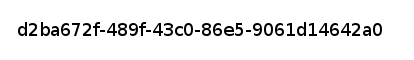
\includegraphics[scale=0.5]{../figures/uuid.png}}
     \caption{The format of a UUID in hex digits is 8-4-4-4-12 for a total of 36 characters}
     \label{fig:uuid}
\end{figure}

Since the length of a UUID is 128-bits, the number of unique ids that can be generated are $2^{128}$. Even though in theory it is possible for a collision between two generated ids to exist, by using strong generation mechanisms, the actual probability of such a collision happening is almost 0. The UUID specification defines five versions which utilize different generation schemes for producing ids, from concatenating the host's MAC address and some time-stamp information to feeding host related information in hash functions like $MD5$ and \textit{SHA-1}. The generation of UUIDs in this project is achieved by using the version 4 scheme, which relies on random numbers. Java provides an implementation of version 4 unique identifiers through the method \textit{randomUUID()} of class \classname{java.util.UUID}. \\

The \classname{Session} class has also been made thread-safe. In the current implementation there is no way of an exception of type \classname{ConcurrentModificationException} occurring since this class is always modified by a single thread. However, it is possible that future versions of the protocol implementation will allow concurrent modification of \classname{Session} objects in order to increase performance and thus, it is useful to have implemented the class from the beginning with these requirements in mind.
\end{description}



\subsection{Integration Layer}
\label{sec:integration_l}

As discussed in Chapter \ref{sec:architecture}, the \textit{Integration Layer} is the component of the protocol, which is responsible for converting all the technical details related to the overlay network into an abstract representation required by the \textit{Control Layer}. We also divided this layer into two "sub-layers", namely the \textit{Abstract Interface} and the \textit{Implementation details}, which conceptually allow us to better explain the connection of our software to the overlay network. In this section we analyze the details of our implementation and we provide two examples of very popular supported overlay networks as a proof of concept, demonstrating the simplicity of porting our software into new network types. 

\subsubsection*{Abstract Interface}

The top sub-layer of the \textit{Integration Layer} is the \textit{Abstract Interface}. As already discussed, this sub-layer is composed by a single component which provides the generic interface with which the control layer interacts in order to receive network related information in an abstract representation.\\

This abstract representation of the underlying network is achieved in Java with the use of the \classname{Node} interface of Listing \ref{lst:node_interface}. This interface defines 3 very simple methods, which can provide to the \textit{Control Layer} with all the required information. These methods are:

\begin{itemize}
\item \classname{getLocalId()}: This method provides the upper layer with the id of the underlying node in an abstract \classname{Id} representation.\\
\item \classname{getOutNeighbors()}: This method provides to the \textit{Control Layer} a set containing the out-neighbors of the present node. The \textit{Control Layer} is then responsible for inserting these neighbors into a \classname{PlainNeighborsTable} and for computing the proper values $a_{uv}$ of matrix $A$ for each. \\
\item \classname{removeOutNeighborNode(String id)}: This method is intended as an optimization and even though it is defined in the interface it can be safely ignored by implementing it to always return a value of \classname{false}. Since our library is using its own failure detection mechanism for discovering failed neighbors, it is possible to discover that some neighboring node has failed before the overlay network does (the overlay could be running its own scheduled maintenance task). Thus, this method is used as a hint of the protocol to the underlying network that the node with the specified id is no longer alive and should be removed from any routing table in which it is currently used. The way that this hint is handled after that, is left to the developer of the overlay.\\
\end{itemize}




\begin{lstlisting} [caption=\classname{Node} interface for abstract node representation, label={lst:node_interface}]
public interface Node {

	public Id getLocalId();

	public Set<Neighbor> getOutNeighbors();
	
	public boolean removeOutNeighborNode(String id);
}
\end{lstlisting}

When a developer needs to port the protocol into a different type of network, she can do so by simply implementing this interface and providing the required information (id, list of neighbors etc) as these are defined for that particular network.


\subsubsection*{Implementation details}

The \textit{Implementation details} sub-layer is composed by nothing more than classes implementing the \classname{Node} interface for particular network types. For a better understanding of how this mechanism works, we present in this section two examples of such implementations provided by our software for two very popular overlays, Pastry and Chord.

\begin{description}
\item[Pastry Implementation] \hfill \\

As discussed in the Background chapter, pastry performs all of its routing operations by using three structures: \begin{inparaenum}[\itshape a\upshape)]
\item a \textit{leaf set},
\item a \textit{routing table} and
\item a \textit{neighbors set}
\end{inparaenum}. From these, only the \textit{leaf set} and the \textit{routing table} are used for actually forwarding messages within the network, while in later versions of Pastry, the \textit{neighbors set} is completely omitted.\\

Our software provides support for one of the most popular implementations of Pastry; \textit{FreePastry} from Rice University \cite{FreePastry}. Using the API provided by \textit{FreePastry}, it was very easy to create a class called \classname{PastryOverlayNode}, which implemented the \classname{Node} interface and provided all the required information in only a few lines of code. \\

Every Pastry node is represented in \textit{FreePastry} by an object of type \classname{PastryNode}. All the network related information of a node (e.g. node id, IP address etc.) are stored in an object of type \classname{NodeHandle} assigned to the corresponding \classname{PastryNode}. A subclass of \classname{NodeHandle} used particularly when the underlying physical network is the IP, is \classname{TransportLayerNodeHandle}. Since for our project we require the existence of an IP physical network, we cast the \classname{NodeHandle} into an object of the aforementioned type (line 3). Then, providing the id of the node to the \textit{Control Layer} of the protocol can be achieved in a very simple manner as shown in Listing \ref{lst:get_node_id}. The id returned by the node's \classname{NodeHandle} is converted to a byte array which is then used to create an object of type \classname{Id} (line 4).

\lstset{
  numbers=left,
  stepnumber=1,    
  firstnumber=1,
  numberfirstline=true
}
\begin{lstlisting} [caption=\classname{getLocalId()} implementation for \textit{FreePastry}, label={lst:get_node_id}]
Id localId = null;
NodeHandle handle = localNode.getLocalNodeHandle();
// Cast the NodeHandle to the subclass providing the IP address of the node
TransportLayerNodeHandle<MultiInetSocketAddress> nh = (TransportLayerNodeHandle<MultiInetSocketAddress>) handle;
localId = new Id(nh.getId().toByteArray());
return localId;
\end{lstlisting}

Discovering the out-neighbors of a node can also be achieved in a simple manner through the provided API. The local node (of type \classname{PastryNode}) provides methods for accessing both its \textit{leaf set} and its \textit{routing table}. These data structures are in reality collections of \classname{NodeHandle} objects of remote nodes, which can be used in the same manner as previously explained to get the node's IP addresses and ids. These information can in turn be used in order to create \classname{Neighbor} objects as in lines 4-5 of the example presented in Listing \ref{lst:pastry_out_neighbors}.

\begin{lstlisting} [caption=Adding nodes from the leaf set to the out-neighbors list in \textit{FreePastry}, label={lst:pastry_out_neighbors}]
for (rice.pastry.NodeHandle remoteNode : leafSetNodes) {
	// Cast the NodeHandle to the subclass providing the IP address of the node
	TransportLayerNodeHandle<MultiInetSocketAddress> nh = (TransportLayerNodeHandle<MultiInetSocketAddress>) remoteNoexternalde;
	byte[] nodeId = nh.getId().toByteArray();
	Neighbor n = new Neighbor(nodeId, nh.getAddress());
	outNeighbors.add(n);
}
return outNeighbors;
\end{lstlisting}

All the aforementioned information could be gathered directly through the API provided by \textit{FreePastry} without any modifications in its original source code, requiring in total less than 100 lines of code. Finally, it should be mentioned that the optional optimization method \classname{removeOutNeighborNode(String id)} was also implemented for Pastry easily, since both the \textit{leaf set} and the \textit{routing table} provide methods for removing remote nodes with a specified id.

\item[Chord Implementation] \hfill \\

In the Background chapter we also explained the operation of the Chord overlay, where all the communications among nodes occur by using a data structure called \textit{finger table}, where a list of successors of node $n$ are stored. If $n$ wishes to forward a message, it will do so by using one of the nodes in this table, with the first record of the table being its immediate successor. Thus, the out-neighbors of the node are all the nodes contained in this data structure. \\

In our software, support is provided for an open source implementation of Chord called \textit{Chordless} \cite{Chordless}. The main reason for choosing \textit{Chordless} over other popular implementations (like \textit{Open Chord}) was due to the simple API it provides for handling network information, which fit perfectly the needs of this project.\\

In \textit{Chordless} every local network node is represented by a \classname{Chord} object assigned a unique identifier. As in \textit{FreePastry}, a class named \classname{ChordOverlayNode} implementing the interface \classname{Node} was created. Transforming the local id to an object of type \classname{Id} was very easy, as shown in Listing \ref{lst:get_node_id_chord}. The identifier of the \classname{Chord} node is converted to a byte array, which is then passed as a parameter to the constructor of \classname{Id}.

\begin{lstlisting} [caption=\classname{getLocalId()} implementation for Chordless, label={lst:get_node_id_chord}]
Id localId = new Id(localNode.getIdentifier().toByteArray());
return localId;
\end{lstlisting}

The out-neighbors discovery is again very simple. The local chord node provides its finger table through the method \classname{getFingerArray()} as shown in line 1 of Listing \ref{lst:chord_out_neighbors}. This table is composed of records containing network information for the successors of the local node in the form of \classname{ServerInfo} objects. Once more, the ids of remote nodes are generated exactly as for the local node (line 3). Finally, since the underlying physical network is the IP, we get the \classname{InetAddress} of a \classname{ServerInfo} object by casting the \classname{SocketAddress} it provides to an object of type \classname{InetSocketAddress} (line 5).

\begin{lstlisting} [caption=Adding nodes from the finger table to the out-neighbors list in \textit{Chordless}, label={lst:chord_out_neighbors}]
ServerInfo [] si = localNode.getFingerArray();
for (ServerInfo server : si) {
	Id nodeId = new Id(server.getIdentifier().toByteArray());
	// Cast the SocketAddress provided by the finger table to also provide IP
	InetSocketAddress isa = (InetSocketAddress) server.getAddress();
	Neighbor n = new Neighbor(nodeId , isa.getAddress());
	outNeighbors.add(n);
}		
return outNeighbors;
\end{lstlisting}

The optional optimization method \classname{removeOutNeighborNode(String id)} was not implemented for \textit{Chordless}, since its API did not provide some public method for manipulating the \textit{finger table}. However, as previously explained, a dummy implementation always returning a value of \classname{false} can be used instead, without interfering with the operation of our protocol.

\end{description}

\subsection{Communications}
\label{sec:communications_impl}

The \textit{Communications} component is part of the protocol's \textit{Control Layer} and is responsible for the construction and exchange of all protocol related messages through the IP network. This section explains how these messages are implemented in an efficient manner, providing an infrastructure for porting the protocol easier into different languages. Additionally, the mechanism for sending and receiving messages through the network is presented and its interaction with the \textit{protocol core} is described.


\subsubsection*{Protocol Messages}

The messages of the protocol were implemented using the \textit{Protocol Buffers} (\textit{protobuf}) library and \textit{protoc} compiler by Google \cite{Varda2008}. Protocol buffers is a flexible, efficient and automated solution for serializing and retrieving structured data. They allow the definition of simple data structures in a special definition language and their compilation to produce classes which represent those structures in wide range of programming languages. The compiled classes provide a heavily-optimized code which allows parsing and serialization of messages in a compact format. \\

As already discussed in Chapters \ref{sec:design} and \ref{sec:architecture}, we can distinguish the protocol messages into two major classes, those carrying a value for one of the \textit{Execution} phases and the control messages, which are used to check whether a node is alive. Each one of these message types contains a number of fields carrying all the required related information (e.g. a value, the \textit{SessionId} etc). Since the protocol messages will be fully structured and can be perfectly handled by \textit{Protocol Buffers}, it makes more sense to use this popular and well-tested method, than defining our own message encoding, which would require further testing to prove its efficiency. Additionally, by using this approach, anyone who wishes to port the protocol in a different language can do so easily and by retaining compatibility with the Java-based implementation, since \textit{Protocol Buffers} provides support for a large number of popular languages, like C++ and Python. \\

The messages involved in the protocol are defined in a "\textit{.proto}" definition file and the accompanying \textit{protoc} compiler is used to generate the Java code from the definitions in that file. The message types defined can be seen in Listing \ref{lst:message_types}. There are 6 types of messages defined. Those in lines 3-5 are the ones used by the protocol for either carrying values in some protocol round or for transferring the computed eigenvalues during the \textit{Gossip Round} (\classname{GOSSIP} type) as explained in Chapter \ref{sec:protocol_description}. The type \classname{NEW} is used only from the initiator node, when a new sampling request is made, in order to pass to the protocol the parameters of the sampling, i.e. the number $m$ of \textit{Executions} and the number $k$ of rounds. The way this mechanism works will be further explained in the \textit{Protocol Core} section. The type \classname{LIVENESS\_CHECK} is used in control messages, to probe a node for liveness. Finally, the \classname{REQUEST\_VAL} type is also used in a control message in order to request from a remote node a value that might not have been received due to network related problem, i.e. the message with the value was sent by the remote node, but it never reached its destination.
 

\lstset{
 language = sh,
  numbers=left,
  stepnumber=1,    
  firstnumber=1,
  numberfirstline=true
}
\begin{lstlisting} [caption=Message types as defined in the "\textit{.proto}" file, label={lst:message_types}]
enum MessageType {
	NEW = 0;
	INIT = 1;
	NEXT = 2;
	GOSSIP = 3;
	LIVENESS_CHECK = 4;
	REQUEST_VAL = 5;
} 
\end{lstlisting}

Apart from the message types, the fields contained in the messages are also defined in the "\textit{.proto}" file and can be seen in Listing \ref{lst:message_fields}. Every field has a keyword (\textit{required}, \textit{optional}, \textit{repeated}), which is used to denote whether and how that field should appear on a message. The \textit{required} keyword denotes a mandatory field, the \textit{optional} keyword an optional field and the \textit{repeated} keyword an optional field that might be repeated multiple times, i.e. an optional list of fields of the same type. All the fields of the messages defined in our protocol are optional, apart from the \textit{type} field. The reason for this is that not all messages contain all the fields defined in the \textit{proto} file. By using the \textit{required} keyword, these fields would be appended to any constructed message, resulting in a message bloated with uninitialized fields. 
	
\begin{lstlisting} [caption=Fields of messages as defined in the "\textit{.proto}" file, label={lst:message_fields}]
required MessageType type = 1;
optional string nodeId = 2;
optional string session = 3;
optional int32 execution = 4;
optional int32 totalNumberOfExecutions = 5;
optional int32 round = 6;
optional double val = 7;
repeated double eigenvals = 8 [packed=true];
\end{lstlisting}

Once the \textit{protoc} compiler is used in the "\textit{.proto}" file, a \classname{ProtocolMessage} class is generated, containing all the methods required for building a message of any of the aforementioned types. This class provides "get" and "set" methods for all the defined fields. The user simply sets the required values to any field that should be part of the message and then calls a \textit{build()} method, to get a message of type \classname{Message}.\\


A problem at this point is that the generated \classname{ProtocolMessage} class allows the construction of messages, which can contain any of the defined fields even if they should not be contained in a message of a particular type. For instance, a \classname{LIVENESS\_CHECK} message could be created, containing an \textit{eigenvals} field, without causing an error, even though it would be semantically wrong. To avoid this situation, a wrapper class \classname{MessageBuilder} was constructed, which provides methods for constructing any type of message, by using only the parameters required by that particular message type. For example Listing \ref{lst:new_message_builder}, shows the method used for generating a message of type \classname{NEW}. This message only requires the number of rounds and executions and using the \classname{MessageBuilder} class ensures that the message will be properly constructed.

\lstset{
 language = Java,
  numbers=none,
  stepnumber=1,    
  firstnumber=1,
  numberfirstline=true
}
\begin{lstlisting} [caption=Fields of messages as defined in the "\textit{.proto}" file, label={lst:new_message_builder}]
public static Message buildNewMessage(int numOfExecutions, int numOfRounds) {
	Message m =
			Message.newBuilder()
			.setType(MessageType.NEW)
			.setTotalNumberOfExecutions(numOfExecutions)
			.setRound(numOfRounds)
			.build();
	return m;
}
\end{lstlisting}

\subsubsection*{Message Exchange Mechanism}

The last part of the \textit{Communications} component is the mechanism for exchanging the messages. We can distinguish this mechanism into two parts, the way messages are sent and the way messages are received. While the protocol is executing, performing samplings, all sorts of messages can be traveling in the network. Obviously, in order to increase the protocol's performance, sending and receiving these messages should be concurrent events, i.e. different threads should be executing for each task independently.\\

\begin{description}
\item[Sending Messages] \hfill \\\\
The class responsible for sending messages is \classname{MessageSender}. This class implements the \classname{Runnable} interface and thus, it can be executed in a separate thread. In order to send any message, \classname{MessageSender} requires an object of type \classname{Message} constructed using the \classname{MessageBuilder} and the \classname{InetAdrress} of the target node. These information are provided by the protocol core, wrapped up in an object of type \classname{TransferableMessage}. This object has additionally a \textit{sendReliably} boolean flag, which defines whether the message should be sent reliably using a TCP connection or if a UDP transmission is acceptable. The initial approach was to send all the messages reliably through TCP without classification. However, since the protocol can send a large amount of messages in a very small period of time, this approach would consume a lot of resources fast. Thus, instead of sending all the messages reliably, only the \classname{INIT} messages are sent that way, because it is important to ensure that they are received, since they will allow a node to discover its in-neighbors. Then, the rest of the messages can be sent through UDP without worrying about them getting lost, since a node can always make a request for a retransmission of an expected message (message of type \classname{REQUEST\_VAL}) if it has not been received after some period of time, as long as its in-neighbors are known. Using this approach and depending on the desirable level of reliability a TCP socket or a datagram is constructed and the message is sent. The protocol defines a constant \classname{PROTOCOL\_PORT} for the port of the remote node in which the message should be sent. The default port currently defined is 11990. \\

A challenge we faced at this point is that when a remote node needs to be probed for liveness, the operation should be blocking, in contrast to sending a message of any other type. The reason for this is that when the protocol core requests to know whether a node is alive or not it needs to get an answer before proceeding, as this will determine whether the remote node's timer should be renewed or the node should be removed from the in-neighbors list. To achieve this, a \textit{makeLivenessCheck()} method is implemented separately and can be executed from the thread of the protocol core, i.e. it is not a part of the \classname{MessageSender}'s \textit{run()} method. As Listing \ref{lst:liveness_check} shows, this method creates a UDP datagram for a \classname{LIVENESS\_CHECK} message and sends this message to the target node. It then sets a timer and waits to receive a reply from the remote node. If a reply is received, a \classname{true} value is returned to the caller (the protocol core). If no reply is received within the defined period, the message is resent. After a number of failed attempts (3 by default), a \classname{false} value is returned to the caller and the remote node is considered dead. It must be noted, that this method does not guarantee that a node reported dead has actually failed. It might be the case that the network was simply congested and all the messages were dropped. However, by properly adjusting the number of failed attempts to the network's characteristics, this method can be effective. For instance, a large network with high traffic and slow connections might require a greater number of failed attempts in contrast to a smaller and faster network.  


\begin{lstlisting} [caption=Simplified snippet of the \textit{makeLivenessCheck()} method., label={lst:liveness_check}]
do{
	// Send a LIVENESS_CHECK message to remote node
	socket.send(datagramPacket);
	try {
		// Wait for 3 seconds for a reply
		socket.setSoTimeout(3000);
		socket.receive(datagramPacketReply);
		// Received a reply. Node is alive
		return true;
	} catch(SocketTimeoutException ste) {
		// Timer expired. Increase number of failed attempts
		numOfTries++;
	}
} while(numOfTries<=3);
// 3 failed attempts. Node is probably not alive
return false;
\end{lstlisting}
\item[Receiving Messages] \hfill \\\\
As previously discussed, messages of the protocol can be sent either using UDP or TCP depending on the defined reliability level. This means, that we need to separate threads for receiving messages, one listening for TCP connections and one expecting UDP datagrams. For TCP connections, a \classname{MessageReceiver} class was created, which opens a \classname{ServerSocket} and awaits for incoming connections in port \classname{PROTOCOL\_PORT}. Any received message is then forwarded to the \textit{protocol core}. \\

In the same manner, a \classname{LightMessageReceiver} class was created for managing UDP datagrams. A \classname{DatagramSocket} expects datagrams from port \classname{PROTOCOL\_PORT} and forwards them to the \textit{protocol core}. If the message is of type \classname{LIVENESS\_CHECK}, then instead of forwarding it, an empty datagram is sent as a reply to the sender in order to prove that the node is still alive. \\

Both classes implement the \classname{Runnable} interface, so that they can be executed in different threads. An additional comment regarding the receiving mechanism is that in the current implementation, the port listening for incoming messages is the same for all the nodes (i.e. \classname{PROTOCOL\_PORT}). This means that virtual nodes are currently not supported by the protocol, since such a feature would require assigning different ports to each virtual node running on the same machine and thus a discovery mechanism for locating each node's listening port would be required.
\end{description}

Another challenge that we faced when designing the communications mechanism is that we do not expect the participating components to have the same workload all the time. For instance, there might be cases in which a node receives a large number of messages in a short period of time, while there might be periods of time with little or no traffic at all. In the same manner, the protocol core is expected to send messages in bursts, e.g. when a new protocol round begins messages should be sent to all the out-neighbors of a node and until the new round ends, little or no other messages need to be transmitted. This means that a synchronization mechanism should be introduced amongst the participating threads to organize and coordinate their execution.\\

\begin{figure}[h]
   \centering
    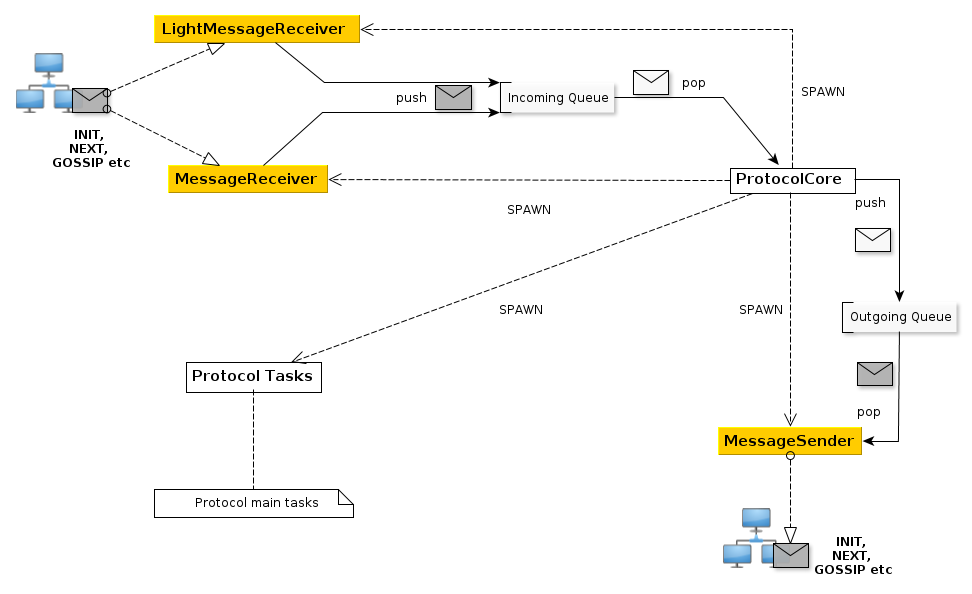
\includegraphics[scale=0.45]{../figures/communication_architecture.png}
     \caption{Synchronization among, sender, receiver and protocol core classes}
     \label{fig:communications_architecture}
\end{figure}

To solve this problem the mechanism illustrated in Figure \ref{fig:communications_architecture} was introduced. When the protocol library is initiated, one of the threads running in the protocol core creates two queues of type \classname{BlockingQueue}, one intended for the incoming messages and one for the outgoing. It then creates 3 new threads; one for each message receiving class, \classname{MessageReceiver} and \classname{LightMessageReceiver}, and one for the sending class \classname{MessageSender}. Then, the protocol core thread blocks on the incoming queue waiting to receive a message. Once a message arrives to any of the receiver classes it is pushed in the incoming queue and it is handled by the protocol core. On the other hand, the message sender is blocked on the outgoing queue waiting to receive an outgoing message. Once the protocol core tasks have some message for one of the node's out-neighbors, the message is placed in the outgoing queue and the sender unblocks and sends the message.\\

Finally, an optimization was made to the way messages are sent, to further improve the protocol's performance. When a message needs to be sent reliably through TCP, a timer is set in the \classname{Socket} used to communicate with the remote node. If the timer expires and a connection has not been established yet, the message is placed in the back of the outgoing queue in order to be resent later. The idea is that if the remote node is very slow or has received two many messages in a short period of time, it might take too long for a connection to be properly established and in the mean time a lot of messages might have been gathered in the local node's sending queue. Then, some remote nodes might be delayed from proceeding to their next round only because they have to wait for a connection with a slower node to be established first by their in-neighbor, before their own message can be sent. However, using a timer would allow the \classname{MessageSender} to send messages faster to responding nodes and then deal with the ones that are slower, which might in turn allow some nodes to terminate faster in the long run.\\

One final remark at this point is that the value of this timer has to be set carefully. If the value is too short, then it could degrade the protocol's performance instead of improving it by not sending messages even to responsive nodes. If on the other hand the value is to big, it could force the \classname{MessageSender} to wait for a very long time, effectively worsening the previously described problem. In our implementation this value has been set to 6000 milliseconds, even though smaller values might also be acceptable (2-3 seconds). 

\subsection{Algorithms and Analysis}
\label{sec:algorithms}

This component is very simple compared to the others, since it only provides implementations for the linear algebra related algorithms required by the protocol. It is composed of only two classes, namely \classname{Algorithms} and \classname{Analyzer}. The \classname{Algorithms} class provides an implementation of Kung's realization algorithm and methods for computing eigenvalues of matrices, while the \classname{Analyzer} class contains all the methods related to the analysis of the estimated eigenvalues to infer useful network properties.\\

\subsubsection*{Algorithms}

All the computations performed by the \classname{Algorithms} class involve operations on matrices. For instance Kung's realization algorithm, which was presented in Chapter \ref{sec:kung}, requires the creation of a Hankel matrix from the impulse responses, its analysis using SVD and then some matrix inversions and multiplications. In order to perform all the required computations efficiently the \textit{jblas} library was used \cite{braschmuejug10}. \textit{jblas} is a linear algebra library for Java, based on the industry-standard libraries for matrix computations, \textit{BLAS} and \textit{LAPACK}. It essentially acts as a wrapper around the routines provided by those libraries to make them Java compatible and performs computations faster than other related projects (e.g. \textit{JAMA}).\\

A point of interest regarding Kung's realization algorithm is the way the order of the surrogate system realization is computed. As explained in Chapter \ref{sec:kung} once the Hankel matrix  of the impulse responses is constructed and singular value decomposition is performed, we end up with three matrices, $U$, $S$ and $V$, such that 

\begin{equation*}
H = USV^T
\end{equation*}

These matrices are then partitioned into sub-matrices for which the number of rows and columns is defined by the order $p$ of the surrogate system. The value of $p$ depends on the number of singular values of $H$ that are above some threshold $thres$. In out implementation, our initial approach was to set a constant value to this threshold, $thres = 1e-7$. However, since the singular values are different depending on the size of the network, making this threshold change dynamically based on the singular values seems to yield better results. For example, consider a case where the first singular value is much larger than the last few. A constant threshold like the aforementioned would probably work well, since the smaller singular values do not carry a lot of information regarding the structure of the system and could be omitted. On the other hand, when all the singular values including the first one are small, then omitting some values using a constant threshold, might result in the loss of useful information. If instead the threshold is relative to the first singular value, the last singular values are omitted only in case they are significantly smaller. In our final approach the threshold was set to $1e-5*s_1$, where $s_1$ is the largest singular value of $H$. \\

A result of the way the order $p$ is computed is that there might be nodes that for the same \textit{Execution} realize systems of a different order. This is because different nodes can gather different impulse responses, which in turn create different Hankel matrices having different singular values. This is also the reason for the approach taken when computing median values in the \textit{Gossip Round} and once a \textit{Session} terminates, where only the $k$ largest eigenvalues of each proposal are taken into account, where $k$ is the size of the shortest proposed vector of eigenvalues (Section \ref{sec:basic_domain}).\\

The rest of the methods in the \classname{Algorithms} class are simple wrappers, which perform any matrix related operation (e.g. computing eigenvalues) by using the \textit{jblas} library and returning the matrices in a double array format. The reason that these wrapper methods are provided and \textit{jblas} is not used directly by the protocol core is to be in line with the extensibility requirement. Using such wrapper functions will allow the easy substitution of \textit{jblas} with another, potentially faster, linear algebra library in the future. 

\subsubsection*{Analyzer}
 
The \classname{Analyzer} class currently supports the estimation of two metrics, the \textit{spectral gap} and the \textit{mixing time}. As explained in Chapter \ref{sec:decentralized_algo}, the \textit{spectral gap} is the difference  $|\lambda_1 - \lambda_2|$ between the two eigenvalues with the largest moduli and since the transition probability matrix we use in our model is stochastic, we have that $\lambda_1=1$ and thus the spectral gap becomes 1-$|\lambda_2|$. Also, the \textit{mixing time} can be approximated by $t_{mix} = \log _{|\lambda_2|}\epsilon$, where $\epsilon$ is the desired error of our estimation.\\

The methods provided by this class are not used directly by the protocol core classes. The protocol core receives sampling requests and returns the estimated eigenvalues, which can then be provided as parameters to any of the methods in the \classname{Analyzer} class to compute some network property. The reason for this approach is to allow the easy extension of the protocol with new analysis capabilities, without tampering with the code of the protocol's core. If all of the analysis computations were performed in the protocol core, then every user who wanted to add some new eigenvalues-based analysis would have to alter the protocol core's functionality, which could potentially break the software. Instead, using this approach, any user can add her analysis method in the \classname{Analyzer} class and then provide the estimated eigenvalues by the protocol core as an input to compute the desired property. The result is much cleaner code and separation of the analysis part from the basic eigenvalues estimation, as illustrated in Figure \ref{fig:analyzer_estimations}.


\begin{figure} [H]
   \centering
    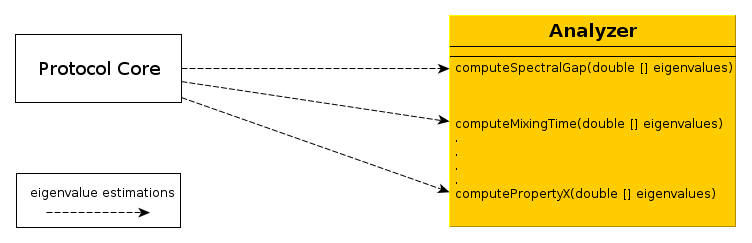
\includegraphics[scale=0.6]{../figures/analyzer.png}
     \caption{Connection of the \classname{Analyzer} class to the protocol core}
     \label{fig:analyzer_estimations}
\end{figure}



\subsection{Protocol Core}
\label{sec:protocol_core}

This component contains all the classes responsible for the coordination and execution of the protocol's operations. It acts as a "control center", utilizing all the components presented so far, in order to perform the requested network samplings and provide eigenvalue estimations to the user. The classes of this component can be divided into three categories: \begin{inparaenum}[\itshape a\upshape)]
\item those performing the main protocol tasks;
\item those responsible for the coordination of these tasks; and
\item the ones responsible for the interaction with the user.
\end{inparaenum}


\subsubsection*{Protocol tasks}

The protocol tasks are all the algorithm-related operations of the protocol, presented formally in the protocol design (Chapter \ref{sec:design}). All these operations are performed by two classes, \classname{MessageHandlerTask} and \classname{MaintenanceTask}.

\begin{description}
\item[MessageHandlerTask] \hfill \\\\
This class is responsible for handling all the messages received by the out-neighbors of the node  apart from the \classname{LIVENESS\_CHECK} messages, which as previously discussed, are directly handled by the \textit{Communications component}. It implements the \classname{Runnable} interface, so that it can be executed in a separate thread and requires three parameters to operate. The first is an object of type \classname{Message}, which is any protocol-related message that needs handling. The second parameter is a list of active \classname{Session} objects, i.e. all the currently running \textit{Sessions} of the protocol. This list is used to locate the \classname{Session} and the \classname{Execution} for which the message is intended, or to add a new \classname{Session} if the received message is of type \classname{NEW} or \classname{INIT}. Finally, the third parameter is the queue of outgoing messages, which is connected to the \classname{MessageSender} and is required in order to send any protocol-related messages to the out-neighbors of the local node, e.g. to send \classname{INIT} messages in the case a new \textit{Session} has been initiated after the node received a message of type \classname{NEW}.\\

Every time a message is received by some in-neighbor, an object of type \classname{MessageHandlerTask} is created and runs in a separate thread. This task performs a check to the type of the message and executes a different handling method accordingly, as shown in Listing \ref{lst:message_handler}. The methods presented in the Listing, are nothing more that the implementations of the message handling tasks described in the protocol design (Chapter \ref{sec:design}). \\

\begin{lstlisting} [caption= Properly handling a message in the \classname{MessageHandlerTask}, label={lst:message_handler}]
switch (incomingMessage.getType()) {
	case NEW:
		this.createNewSession();
		break;
	case INIT:
		this.handleInitMessage();
		break;
	case NEXT:
		this.handleNextMessage();
		break;
	case GOSSIP:
		this.handleGossipMessage();
		break;
	case REQUEST_VAL:
		this.resendVal();
		break;
	default:
		logger.warning("The message was malformed. Dropping...");
		break;
}
\end{lstlisting}



The only method that needs some further explanation is \textit{resendVal()}, which is executed when a message of type \classname{REQUEST\_VAL} is received. As already discussed, all the messages apart from those of type \classname{INIT} are sent unreliably through UDP, which means that it is possible for a message of a particular round to get lost. When a remote node realizes that one of its in-neighbors has not sent a value even though it is still alive, it assumes that the message has been lost and it sends a \classname{REQEUEST\_VAL} to ask for a retransmission. The \classname{MessageHandlerTasks} is then responsible for resending the requested message.\\

A pitfall at this point is that a node might have made a retransmission request, believing that a message was lost, while the message could have just been delayed. The result of this would be to end up with the same message twice, which could lead to computing a wrong impulse response and in turn to make wrong estimations. However, the message handling task has been implemented in such a manner, that duplicate messages can be recognized and ignored, by maintaining a minimal archive of all the received messages for a particular \textit{Execution}, as Table \ref{table:pending_values} illustrates. When a message of a particular round of an \textit{Execution} is received, the sender is marked as seen. If a message from the same in-neighbor and round of an \textit{Execution} is received a second time, it can be safely ignored. For example using the values of Table \ref{table:pending_values}, if a message is received by \textit{node1} for round 2, it will be ignored, while a message for the same round by \textit{node2} will be accepted. This action is performed atomically, which means that there is no way for a duplicate message to be accepted twice. 

\begin{table}[H]
\centering
\begin{tabular}{|c|c|c|}

\hline
\multicolumn{3}{|c|}{\textit{Execution} $x$} \\
\hline
\hline
In-Neighbor Id & Round & Status\\
\hline
\textit{node1} & 1 & seen \\
\textit{node2} & 1 & seen \\
\textit{node1} & 2 & seen \\
\textit{node2} & 2 & pending \\
\hline

\end{tabular}
\caption{Table of pending a received values for \textit{Execution} $x$}
\label{table:pending_values}
\end{table}


\item[MaintenanceTask] \hfill \\\\
This class is responsible for performing the maintenance tasks of the protocol. Similar to \classname{MessageHandlerTask}, it implements the \classname{Runnable} interface, so that it can be executed in a separate thread, and also accepts as parameters a list of the active \classname{Session} objects and the queue of out-going messages connected to the \classname{MessageSender}.

When a \classname{MaintenanceTask} runs, it iterates over the list of active \textit{Sessions} and checks its \textit{Executions}. For each \textit{Execution}, the maintenance tasks described in protocol design (Chapter \ref{sec:design}) are performed. These tasks include the updating of the in-neighbors' timers, the discovery of failed in-neighbors by probing nodes for liveness and the advancement of \textit{Executions} in later rounds if all required messages have been received.\\

\begin{lstlisting} [caption= Probing for liveness and requesting retransmission of a value, label={lst:request_val}]
// Check whether the node is alive 
if (inNeighbor.getTimeToProbe() <= 0) { 
	if (isAlive(inNeighbor)) {
		/* The node is alive. Renew its timer and 
		   request a retransmission for the current round */
		inNeighborsTable.renewTimer(inNeighbor);
		requestPreviousVal(sessionId, executionNumber, executionRound, address);
	}
}
\end{lstlisting}

Additionally, this class is responsible for sending \classname{REQUEST\_VAL} messages to its in-neighbors as shown in Listing \ref{lst:request_val}. When the timer of a node expires, it means that the node should be probed for liveness. If a node replies to the probing, it verifies it is still alive, which means that the reason for not having its timer set to $INF$ could be that the value it has sent for the current round was lost due to the unreliable transmission. Thus, a request for a retransmission of the message for that particular round is made. As previously explained, even if the message was simply delayed and not lost, this action could not cause any harm to the proper computation of the impulse responses; the only disadvantage is that it incurs some additional overhead due to the extra messages sent.



\end{description}



\subsubsection*{Tasks Coordination}

The coordination of the aforementioned protocol tasks and the \textit{Communication component} is performed by the \classname{ProtocolController} class. When the protocol is initiated, an object of this class is created, running on a separate thread. This thread spawns three additional threads, one running the \classname{MessageSender} and the other two running the \classname{MessageReceiver} and \classname{LightMessageReceiver} services. At the same time, it creates two \classname{BlockingQueues}, one for the incoming messages and one for the outgoing and passes them as parameters into the communication threads. Then it schedules an additional thread to run with a fixed delay of one second between consecutive executions, performing the operations of the \classname{MaintenanceTask}. It then goes on an infinite loop, performing the actions illustrated in Figure \ref{fig:protocol_controller}. 

\begin{figure} [H]
   \centering
    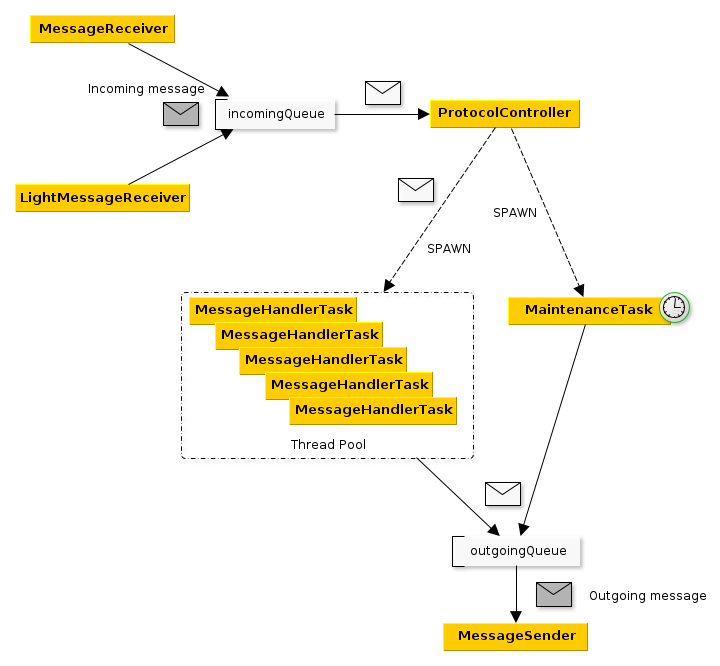
\includegraphics[scale=0.5]{../figures/protocol_controller.png}
     \caption{Coordination of protocol tasks by the \classname{ProtocolController} class}
     \label{fig:protocol_controller}
\end{figure}

The \classname{ProtocolController} blocks on the incoming queue, waiting to receive a new message. When a message arrives to either of the receiving threads, it is pushed in the queue and the controller is unblocked. The incoming message is  then assigned by the controller to a \classname{MessageHandlerTask}, which performs the operations described previously. Since a lot of messages can arrive in a small period of time and in order to improve the protocol's performance, instead of using only one thread running a \classname{MessageHandlerTask}, the controller has a pool with a fixed number of threads, which allows it to execute multiple \classname{MessageHandlerTasks} concurrently. In the current implementation the thread pool is set to provide up to 5 threads simultaneously. It should be noted at this point, that since the \classname{Execution} class has been made thread-safe, there is no problem following this approach, since \classname{MessageHandlerTask} objects can now access the same \classname{Execution} concurrently without worrying for concurrent modification exceptions.\\


\subsubsection*{User interaction}

The interaction of the user with the protocol is achieved through the \classname{ProtocolEngine} class. This class is responsible for initializing the protocol and providing an API for the user to make sampling requests. The only parameter required for the creation of the protocol engine is an object of type \classname{Node}, i.e. an object of one of the classes provided by the \textit{Integration Layer}. This abstract node will be used to bind the protocol to the network over which it is expected to run. For example, Listing \ref{lst:protocol_engine_initialization} shows an example of a \classname{ProtocolEngine} initialization for an application running on top of a Pastry overlay using \textit{FreePastry}. Initially a pastry node is created as it would in any application using \textit{FreePastry} (lines 2-3). This pastry node is then passed as a parameter to an object of type \classname{PastryOverlayNode}. As explained in Section \ref{sec:integration_l}, the class \classname{PastryOverlayNode} implements the interface \classname{Node} and integrates the protocol to a \textit{FreePastry} application. This object is then used by the \classname{ProtocolEngine} as previously mentioned, so that the protocol can be initialized (line 7). Finally, the normal operation of the application is resumed and the pastry node joins the overlay (line 9). This example, demonstrates the simplicity with which the library can be integrated into any application (with only two lines of code), as long as the proper integration layer class is implemented.\\

\lstset{
 language = Java,
  numbers=left,
  stepnumber=1,    
  firstnumber=1,
  numberfirstline=true
}
\begin{lstlisting} [caption=Initialization of \classname{ProtocolEngine} over \textit{FreePastry}, label={lst:protocol_engine_initialization}]
// construct a pastry node
PastryNodeFactory factory = new SocketPastryNodeFactory(nidFactory, bindport, env);
PastryNode node = factory.newNode();
// construct a connector to be used by the protocol library
PastryOverlayNode pon = new PastryOverlayNode(node);
//create the protocol engine
ProtocolEngine pe = new ProtocolEngine(pon);
//boot the pastry node
node.boot(bootaddress);
\end{lstlisting}



\noindent The \classname{ProtocolEngine} performs two operations while initiating:
\begin{description}
\item[First] It opens (or initializes if not already existing) the database where previous \textit{Session} data of the application are stored. This database will be used to store the results of future samplings and to make a decision whether a new sampling should be performed or not using an algorithm that will be presented later in this section. \\
\item[Second] It creates an object of type \classname{ProtocolController}. The \classname{ProtocolController} runs as a daemon service, and as already explained is responsible for synchronizing the communication threads with the classes performing the \textit{Session}-related tasks of the protocol.  \\
\end{description}   

Finally the \classname{ProtocolEngine} provides a simple API which can be used for making sampling requests. The methods provided by this API accept as parameters the number of \textit{Executions} the requested \textit{Session} should contain and the number of rounds in each one of them. The sequence of actions performed when a user makes a request can be seen in Figure \ref{fig:unser_interaction}. When the user makes the request, the \classname{ProtocolEngine} creates an object of type \classname{ProtocolRun}, which runs in a separate thread. This object is responsible for creating a message of type \classname{NEW} with the parameters of the new sampling request. This message is forwarded to the \classname{ProtocolController} through the queue of incoming messages and the \classname{ProtocolRun} object blocks, waiting to receive a reply. Once the sampling is over, the \classname{ProtocolController} stores the computed \textit{Session} in the database and the \classname{ProtocolRun} is notified that the sampling is over. Finally, the computed \textit{Session} is passed to the \classname{ProtocolEngine}, so that it can be returned to the user.\\

\begin{figure}
   \centering
    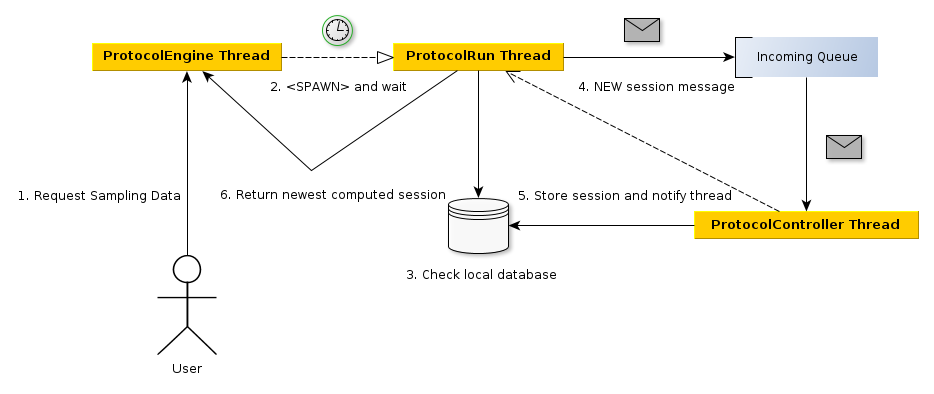
\includegraphics[scale=0.5]{../figures/user_interaction.png}
     \caption{User interaction with the sampling protocol}
     \label{fig:unser_interaction}
\end{figure}

The notification mechanism used for informing a \classname{ProtocolRun} that a sampling request is over is based on \textit{Event Listeners}. More specifically, the \classname{SessionListener} interface presented in Listing \ref{lst:session_listener_definitions} was created. This interface defines three methods related to the different events that might occur in the life-cycle of a \textit{Session} and acts as an \textit{Event Handler}. When a \classname{Session} is initiated or terminates, a \classname{SessionEvent} is created, containing basic information of the \classname{Session}, i.e. \textit{SessionId}, number of \textit{Executions}, ids of out-neighbors etc. This event and the methods that handle it are related to the evaluation mechanism, which will be presented later in this Chapter and have no relation to the \classname{ProtocolRun}. The event that is of interest to us is the \classname{RecordedSession}. A \classname{RecordedSession} is an event created by the storage component once a terminated \classname{Session} is successfully stored and provides the \classname{Session} object having the estimation and a timestamp of the event's occurrence. The \classname{ProtocolRun} fully implements only the \textit{sessionStored()} event handler of the \classname{SessionListener} interface. The other two methods are left void, since they are of no interest at this point.\\

\begin{lstlisting} [caption=\classname{SessionListener} interface, label={lst:session_listener_definitions}]
public interface SessionListener {

	// This is called when the Session is initiated
	public void sessionInitiated(SessionEvent e);
	// This is called weh the Session terminates
	public void sessionCompleted(SessionEvent e);
	// This is called once the Session is stored in the storage component
	public void sessionStored(RecordedSession rs);
	
}
\end{lstlisting}

As already mentioned, the \classname{ProtocolRun} makes a sampling request to the \classname{ProtocolController} and then blocks on a \textit{lock} waiting for the \textit{Session} to terminate. Once the sampling is over and the storage component has it stored, it calls the \textit{sessionStored()} handler, passing it the \classname{RecordedSession} as a parameter. As it can be seen in Listing \ref{lst:session_stored}, the only actions performed by this method are to provide the terminated \classname{Session} to the listening \classname{ProtocolRun} and to notify it that the sampling is over by signaling the aforementioned \textit{lock}. When the \classname{ProtocolRun} thread awakens, it simply returns the \classname{Session} to the \classname{ProtocolEngine} and terminates.  

\begin{lstlisting} [caption=Implementation of the \textit{sessionStored()} method by \classname{ProtocolRun}, label={lst:session_stored}]
public void sessionStored(RecordedSession rs) {
	synchronized (lock) {
		// The RecordedSession is passed to the ProtocolRun
		s = rs.getRecordedSession();
		// The ProtocolRun thread is notified to wake
		lock.notify();
	}
}
\end{lstlisting}

\subsubsection*{Sampling Optimization}

At this point, an optimization was introduced in order to reduce the network traffic caused by the protocol samplings. The idea is that if a network is relatively stable, then consecutive samples with a small time interval would probably provide the same estimations, since the network structure will have remained unchanged. Thus, instead of allowing a new sampling process to be initiated every time a sampling request is made, we could dynamically adjust the sampling intervals depending on the current behavior of the network. In order to achieve this, we define a $current\_threshold$, which dictates what the time interval between two sampling processes should be. As Algorithm \ref{alg:sampling_init} demonstrates, when a new sampling request is made, we check how much time has passed since the last sample was taken and we compare this with the $current\_threshold$. If the elapsed time is less than the $current\_threshold$, then the previous estimation is returned, otherwise a new sampling process is initiated.

\floatname{algorithm}{Algorithm}
\setcounter{algorithm}{2}
\begin{algorithm}
\caption{Sampling initiation algorithm}
\label{alg:sampling_init}
\begin{algorithmic}[1]
\STATE $t \leftarrow$ time of the previous sampling
\IF {current time $-t$ $>current\_threshold$}
\STATE Initiate a new sampling process
\ELSE
\STATE Return the previous sampling estimation
\ENDIF 
\end{algorithmic}
\end{algorithm}		

\noindent The $current\_threshold$ is adjusted dynamically, using a very simple mechanism. Initially, it is set to a minimum value of $minimum\_threshold$. When a sampling terminates, its estimated eigenvalues are compared to the estimations of the previous sample. If they are the same, this means that there was no change in the network structure and thus the $current\_threshold$ can be increased. The increase is computed as

\begin{equation}
increase = current\_increase\_rate \times current\_threshold
\end{equation}
where the $current\_increase\_rate$ is also initially set to some minimum value $minimum\_rate$. Then, the $current\_threshold$  and the $current\_increase\_rate$ become
\begin{eqnarray}
current\_threshold = increase + current\_threshold \\
current\_increase\_rate = current\_increase\_rate+ rate\_step
\end{eqnarray}
where $rate\_step$ is a small value, e.g. 0.05. As we can see, in a stable network the sampling intervals become longer with an ever increasing rate, which means that as time progresses the samplings will be continuously reduced. \\

However, even in stable networks samples have to be taken from time to time in order to make sure that no changes have occurred. Thus, in order to prevent the $current\_threshold$ from becoming really large (no sample will be ever taken), we set an upper bound value $max\_threshold$, where the sampling intervals will once more stabilize. \\

When the compared estimations of the samplings are different, some kind of topological change must have occurred to the network, either due to node failures or from nodes joining in and departing from the network. In this case the $current\_threshold$ and the $current\_increase\_rate$ are reset back to their minimum values. This will make the sampling intervals short again, allowing us to take more samples of the network in order to evaluate its new behavior.

\subsection{Storage}

The final component of the protocol is related to \textit{Storage}. As already mentioned, storing the previous protocol estimations is essential both for regulating the frequency of new sampling requests and for using them for analysis purposes. \\

Storage, as all the protocol's components, can play an important role in the performance of the whole system, especially in cases where a very large amount of estimations is already stored and needs to be retrieved. Depending on the system over which the protocol is deployed, the storage requirements might differ. For instance, there might be systems where simple storage of the estimations in a CSV file might be adequate, while in other cases more complex solutions like relational or temporal databases might be required.\\

In order to offer more extensibility regarding the provided storage capabilities, the \classname{Database} interface presented in Listing \ref{lst:database_interface} was introduced. Any supported storage component should implement this interface, which defines all the required actions that are essential for the protocol to properly function. 

\begin{lstlisting} [caption=The \classname{Database} interface, label={lst:database_interface}]
public interface Database {

	// Add a Session to the database
	public void addSession(RecordedSession rs);
	// Retrieve the last stored Session
	public RecordedSession getLastRecordedSession();
	// Add a SessionListener for monitoring database events
	void addSessionListener(SessionListener listener);
	// Remove the SessionListener
	boolean removeSessionListener(SessionListener listener);
	// Close the database when the protocol terminates
	public void closeDatabase();
	
}
\end{lstlisting}

Storage capabilities are currently provided by our implementation through the use of class \classname{KeyValueDatabase}. This class acts as a wrapper for \textit{jdbm2} library \cite{citeulike:10520984}. \textit{jdbm2} is a key-value database, which provides \classname{HashMap} and \classname{TreeMap} data-structures for storing the \textit{Session} objects, which are backed up by disk storage. The reason this library was used, is that it is a very easy and fast way to persist your data. However, in large deployments where frequent sampling requests might be made, a more complex storage mechanism than \textit{jdbm2} would probably be required.
 

\section{Protocol Evaluator}
\label{sec:evaluator}

Since the protocol we propose will be deployed in a decentralized network, it is important to create a mechanism for the evaluation of our results. For a proper evaluation to be performed, our estimated values should be compared with the actual values. In order to compute the actual values a network node needs to know the structure of the whole network, i.e. it needs to know the number of participating nodes and how these nodes are connected (their links). If the network structure is known, then a node can easily construct the adjacency matrix of the network and it could use this or any other closely related matrix in order to compute the network's actual spectral properties. Unfortunately, since the network is decentralized, each node holds by definition only partial information, which is also the reason we need the proposed decentralized protocol in the first place. More specifically, every node knows only its id and the ids of its out-neighbors, which means that directly constructing the adjacency matrix is impossible.\\

To solve this problem we introduced an evaluation mechanism, which allows a node to learn the structure of the network in order to compute its actual spectral properties. To achieve this we define one node as the \textit{evaluator} and the rest of the nodes as the evaluation \textit{participants}. The \textit{evaluator} is the node controlled by the user, where the experiments will be conducted and the results should be returned. The role of each node is defined by the user beforehand, by providing them the IP of the \textit{evaluator}. Each node simply needs to compare its own IP to the provided one to find out whether it should assume the role of the \textit{evaluator} or the \textit{participant}.\\

Once every node's role has been defined, the user makes queries to the \textit{evaluator} and expects the results. Then, the evaluation mechanism performs two actions. The first is to make a sampling request using the implemented protocol and to store the estimated values. The second is to compute the actual values from the network, by gathering topological information by all the \textit{participants}, as Figure \ref{fig:gather_eval} illustrates. Once the sampling process terminates, all \text{participants} send a message to the \textit{evaluator}, containing all their local topological information, i.e. their id and the list of their out-neighbors. For example node 5, sends a message to the evaluator containing values 4 and 6, since its out-neighbors are the nodes with ids 4 and 6. Using these information, the evaluator can construct the adjacency matrix and any matrix related to it. The computation of the actual network values is then trivial. \\

\begin{figure}
   \centering
    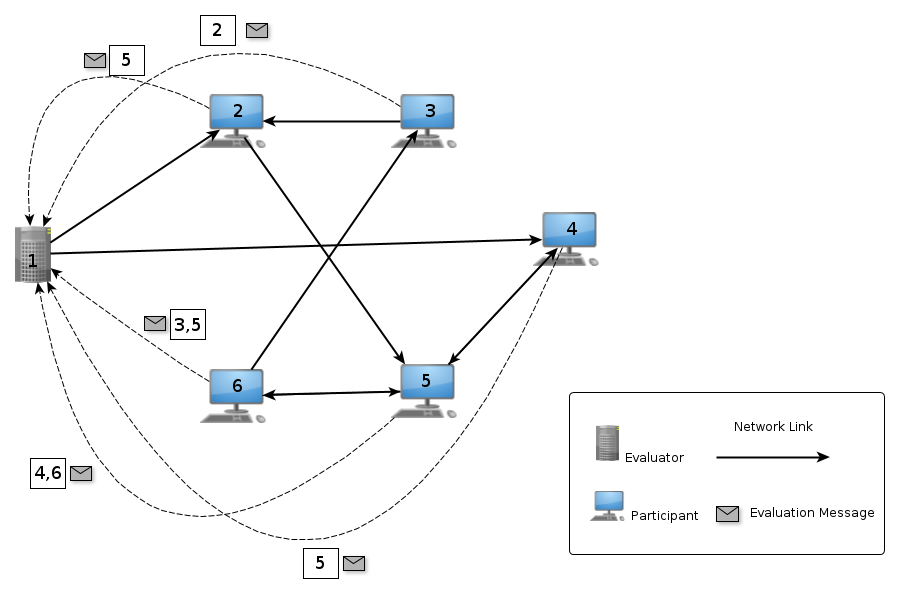
\includegraphics[scale=0.5]{../figures/evaluator.png}
     \caption{Collection of structural information by \textit{evaluator} node}
     \label{fig:gather_eval}
\end{figure}

It should be noted at this point that the aforementioned method works only in case that the network is not very large, e.g. a network of only a few hundred nodes. For networks composed of thousands of nodes, such an approach would probably overload the \textit{evaluator} node, since too many connections would have to be performed at once. However, for the experiments performed in this project this method turned out to be effective and the actual network properties could be computed, as it will be discussed in Chapter \ref{sec:evaluation}.





\section{Deployment and Documentation}

The management of the project's implementation was performed by using \textit{Maven}, a build automation tool mainly used for Java projects. The main advantage of \textit{Maven}, compared to other similar tools, is that it can locate all the project's dependencies through one or more repositories and download them automatically in the local cache, without requiring any intervention by the user. The only dependencies of this project that weren't available in any public repository were the .jar files for \textit{FreePastry} and \textit{Chordless}. For this reason, these files are provided as part of the codebase, located in the \textit{resources} directory of the source code. The protocol can be compiled by issuing in the project home directory (where the \textit{pom.xml} file exists) the following commands:

\begin{verbatim}
mvn clean
mvn compile
\end{verbatim}

\noindent To create a .jar file containing all the class files of the project the following command has to be issued:

\begin{verbatim}
mvn install
\end{verbatim}

\noindent The resulting .jar will not include any dependencies, e.g. \textit{jblas}. To create a .jar file containing all the project's dependencies you have to issue the following command:

\begin{verbatim}
mvn assebly:single
\end{verbatim}

Documentation of the code is provided along the codebase through \textit{Javadoc} which is integrated to the build process. The full documentation can be generated by simply running:

\begin{verbatim}
mvn javadoc:javadoc
\end{verbatim}

\noindent Additional documentation is provided through the unit tests that are also part of the codebase, located in the \textit{test} directory. These tests could be used as examples of how the individual components of the protocol are used in reality, however they provide no additional information regarding the component's synchronization and concurrent execution. These tests can be performed by simply running:

\begin{verbatim}
mvn test
\end{verbatim}

\section{Summary}

In summary, we presented the implementation details of the protocol's constituent components, explaining in-depth their interaction and synchronization mechanisms. Finally, we presented the evaluation mechanism which will be used for the experiments discussed in the next chapter and gave some brief information regarding the protocol's build method and documentation.

\chapter{Evaluation}
\label{sec:evaluation}

In this section we attempt to evaluate the success of this project. An easy way to achieve this is by checking whether the requirements we defined in the protocol design (Chapter \ref{sec:design}) have been met. In addition, we present a realistic scenario, in which our proposed protocol could have practical use, not just as a scientific tool, but for presenting to users useful and interesting statistics. Finally, for completeness, we discuss the limitations that our proposed solution has.

\section{Experimental Setup}

Before attempting to evaluate our results, we need to present our experimental setup. The evaluation methodology and parameters presented here were used throughout all of the conducted experiments of the following sections, unless stated otherwise.\\

As already discussed in the implementation details (Chapter \ref{sec:implementation}), the protocol was implemented with initial support provided for two types of P2P networks, Pastry and Chord, through their open source implementations of \textit{FreePastry} and \textit{Chordless} correspondingly. However, the evaluation of the project was performed only over the Pastry overlay, mainly due to the topological similarities the two overlays share and also because of the time constraints of the project, which did not allow us to thoroughly test our Chord implementation.\\

In order to properly evaluate our results, we required a testbed which could simulate a real network as much as possible. The reason for this is that a real network can present a much different and unpredictable behavior than a simulated environment, which would be useful for strengthening our results. All of our experiments were conducted in \textit{PlanetLab}. \textit{PlanetLab} is a research network, used for development and testing of new network services and is composed of approximately 1000 nodes at about 500 sites spanning across the world. Its power lies in that it runs over the Internet, rendering it far more realistic than a simple simulator.\\

Every \textit{PlanetLab} user is assigned a "slice", i.e. access to virtual machines in a subset of the offered nodes. The user can manage her slice (add or remove nodes) through a simple web interface. Even though managing a slice by using a browser is very simple, it can also be very slow in cases that the user needs to manage a slice composed of a large number of nodes (a hundred or more). As an alternative, an  API is provided, which can be used by scripts to quickly filter the nodes of a slice based on their properties, e.g. the user can define a threshold for the bandwidth or the CPU load the nodes of the slice should have.\\

For the evaluation of our protocol, we used a slice composed of 100 nodes selected at random. This means that these nodes offered various levels of service, e.g. some nodes were very fast with high bandwidth, while others were slower and with very limited bandwidth and memory. Even though selecting only highly performing nodes was an option, the variance in the specifications of participating nodes was required to create a more realistic P2P overlay, since in real networks all kinds of nodes are usually allowed to join.\\

In order to run the implemented protocol, \textit{Java Runtime Environment 7u25} was uploaded and installed in all the participating nodes, along with a .jar file containing the protocol implementation and all of its dependencies. Finally, as described in the implementation of the evaluation mechanism in Chapter \ref{sec:evaluator}, one node was selected at random and was defined as the \textit{evaluator}. This node was used for making sampling requests by passing the desired parameters and it was also the point, where all the evaluation data were gathered and analyzed. \\

Since all of the experiments presented in this chapter were performed in a Pastry overlay network, it would be useful to have a visual perception of how the topologies constructed in such a network look like. Figure \ref{fig:pastry_eval} illustrates a graph constructed using the data gathered by the \textit{evaluator} while performing experiments in a network composed of 20 nodes. As we can see, this topology has a great symmetry, with each node having about the same number of out-neighbors spread over the network ring. Graphs for networks of 50 and 100 nodes were also generated, but they are not presented here, since they produced unclear images due to the large number of edges they contained. However, their results also indicate symmetrical topologies, with all nodes having about the same number of out-neighbors spread over the network ring as presented in Table \ref{table:topology_sizes}.

\begin{table}[b]
     \centering
   	\begin{tabular}{|c|c|}
   	\hline
   \textbf{\textit{Number of Nodes}} & \textbf{\textit{Number of out-neighbors}}\\
   	\hline
   	\hline
   	 20 & 19\\
   	 \hline
     50 & 22\\
     \hline
     100 & 25\\
       \hline
     	\end{tabular}
     	\caption{Number of out-neighbors per node for networks of different sizes}
     	\label{table:topology_sizes}
\end{table}

\begin{figure}
   \centering
    \includegraphics[scale=0.17]{../evaluation_data/topologies/twenty_nodes.png}
     \caption{Example pastry topology of 20 nodes}
     \label{fig:pastry_eval}
\end{figure}

\section{Evaluation of Requirements}

In this section we revisit the requirements set in the design chapter and we evaluate our protocol's performance. This is critical in order to better understand the proposed protocol's strengths and weaknesses.

\subsection{Correctness}

In order to evaluate the correctness of our impulse response protocol implementation, we performed experiments into three networks composed of 20, 50 and 100 nodes respectively. The nodes joined the network one at a time and an idle period was introduced between the construction of the network and the execution of the experiments. This was to ensure that all the nodes have properly joined the network and that their routing tables and \textit{leaf} sets have stabilized, before making any sampling request. Additionally, all the tested networks were without churn, i.e. no new nodes joined the network and no failures or departures occurred.\\

For all the aforementioned networks, we examined two properties computed by using the eigenvalues of the transition probability matrix; their \textit{spectral gap} and their \textit{mixing time}. As a reminder, the \textit{spectral gap} is the difference  $|\lambda_1 - \lambda_2|$ between the two eigenvalues with the largest moduli ($1-|\lambda_2|$ since the matrix is stochastic) and the \textit{mixing time} can be approximated by $t_{mix} = \log _{|\lambda_2|}\epsilon$, where $\epsilon$ is the desired error of our estimation. Both of these properties are considered very important, since they can be used as parameters for algorithms estimating other properties, as we shall later see in section \ref{sec:sampling_app}.\\

For all the experiments, each sampling request was for a \textit{Session} with a single \textit{Execution} ($e=1$). Since the networks were without churn, making sampling requests for multiple \textit{Executions} would not increase the accuracy. The experiments were conducted for various values of parameter $k$ (number of rounds). More specifically, for networks of size 20 and 50, the experiments were performed for $k=1\dots40$ and for networks of size 100 for $k=1\dots50$. \\

Figure \ref{fig:spectral_no_failure} illustrates the spectral gap error for the 10th, 50th and 90th percentile of the estimated values versus the number of gathered impulse responses, i.e. the number of rounds. The blue lines represent the median (50th percentile) and the error bars represent the extremes. As we can see for the 20-nodes network, 5 rounds are enough for the error to drop under $1e-13$ for all the examined percentiles. However, the close-up diagram for rounds $k=5\dots40$ clearly shows that the error never drops exactly to 0 and that it also does not completely stabilize. This instability is probably related to the way the protocol is initialized, since the initial impulse response of each node is selected uniformly at random, leading to different initial network configurations in each execution. The same observations apply to networks of sizes 50 and 100. The only difference is that the 50-nodes network requires about 10-15 rounds to minimize the error and the 100-nodes network requires about 20-30 rounds. A final remark is that as we can see in the close-ups of Figures \ref{fig:spectral_no_failure}b and \ref{fig:spectral_no_failure}c the minimum error for the larger networks is higher (magnitude of $1e10-5 $) compared to the error of the smallest one. However all errors are small enough to prove the correctness of our implementation. \\

Similarly, Figure \ref{fig:mixing_no_failure} illustrates the mixing time error for all networks. Like for the spectral gap, the best mixing time estimations are computed in at most 30 rounds regardless of the network size. As expected, the number of rounds required increases with the size of the network. A difference we can observe in these diagrams is that the error is in general always higher than that of the spectral gap. The reason is that the mixing time is closely related to the spectral gap and thus a small error of the spectral gap could lead to higher mixing time errors. Nonetheless, these results are also noted by Carzaniga et al. \cite{6195806}, verifying the correctness of out results.


\begin{figure}
\centering
\subfloat[spectral gap error in 20 nodes]{
\includegraphics[width=0.6\textwidth]{../evaluation_data/no_failures/spectral_20.png}}
\qquad
\subfloat[spectral gap error in 50 nodes]{
\includegraphics[width=0.6\textwidth]{../evaluation_data/no_failures/spectral_50.png}}
\qquad
\subfloat[spectral gap error in 100 nodes]{
\includegraphics[width=0.6\textwidth]{../evaluation_data/no_failures/spectral_100.png}}

\caption{Spectral gap error for the 10th, 50th and 90th percentile of the estimated values versus the number of gathered impulse responses}
\label{fig:spectral_no_failure}
\end{figure}


\begin{figure}
\centering
\subfloat[mixing time error in 20 nodes]{
\includegraphics[width=0.6\textwidth]{../evaluation_data/no_failures/mixing_20.png}}
\qquad
\subfloat[mixing time error in 50 nodes]{
\includegraphics[width=0.6\textwidth]{../evaluation_data/no_failures/mixing_50.png}}
\qquad
\subfloat[mixing time error in 100 nodes]{
\includegraphics[width=0.6\textwidth]{../evaluation_data/no_failures/mixing_100.png}}
\caption{Mixing time error for the 10th, 50th and 90th percentile of the estimated values versus the number of gathered impulse responses}
\label{fig:mixing_no_failure}
\end{figure}


\subsection{Robustness}

In this section we discuss the robustness of the protocol in the presence of failures or churn. In order to do this properly, we need to analyze different scenarios, in which topological changes could occur for various reasons. Unless stated otherwise, for all the experiments presented in this section, a network of 50 nodes was used. 

\subsubsection*{Single Failure Resistance}

We begin our evaluation by examining the case in which a single failure or departure occurs in the network while the protocol is executing. Before evaluating our proposed fault-tolerant mechanism, we need to analyze the behavior of the protocol in the simple case that each \textit{Session} contains only one \textit{Execution}. To do this, we performed multiple sampling requests, each time using various values for the number of rounds $k$, from 1 up to 40. For every $k$ we used, we ran the experiment multiple times, introducing the failure in a different round each time. For instance, for $k=10$, we ran the experiment 10 times, with the failure occurring at round 1 the first time, at round 2 the second etc.\\

Using the estimated eigenvalues, we computed the network's median spectral gap and mixing time error as before. The results can be seen in the "heat maps" of Figure \ref{fig:single_exec_failure}. Each square of the diagram represents a \textit{Session}, where the values of the x-axis show the number of rounds $k$ and the values of the y-axis show the round in which the failure was introduced. All the elements above the diagonal present \textit{Sessions} for which the failure was introduced after the execution terminated, i.e. the elements above the diagonal are failure-free \textit{Sessions}. The darker the color is in an area, the lower is the error for that particular \textit{Session}. \\

As we can see, \textit{Sessions} near the diagonal have a much higher error than those near the bottom of the diagram. This means that if an error is introduced early in the execution, the protocol has time to recover and provide good estimates. On the other hand, if the failure occurs after $k/2$ rounds, the error can get really high, meaning that stability in the last few collected impulse responses is important for accurate estimations. Finally, we can observe a vertical stripe of high errors in the beginning of each diagram, demonstrating \textit{Sessions} in which the error is very high regardless of the round it was introduced. This is natural, since as we have already seen, the first few rounds (5-10) produce very inaccurate results even in stable networks. All the aforementioned results are as expected and are in league with those presented by Carzaniga et al. \cite{6195806}. 


\begin{figure} [h]
\centering
\subfloat[spectral gap median error]{
\includegraphics[width=0.45\textwidth]{../evaluation_data/single_failure_single_execution/spectral_heatmap.png}}
\qquad
\subfloat[mixing time median error]{
\includegraphics[width=0.45\textwidth]{../evaluation_data/single_failure_single_execution/mixing_heatmap.png}}
\caption{Introduction of a single failure in a network of 50 nodes, using a single \textit{Execution}}
\label{fig:single_exec_failure}
\end{figure}

The next thing that we wanted to test was the behavior of the protocol for a single failure in the case that each \textit{Session} contains multiple \textit{Executions}. For this experiment the failure was always introduced at round $\lfloor \frac{3k}{4} \rfloor$, since our previous results indicated that the error would be higher for a failure at some point after round $k/2$. Also the experiment was performed for \textit{Sessions} containing up to 5 \textit{Executions} and for 10, 15 and 20 rounds. Using these configurations, the average spectral gap percent error was computed.\\

The results of the experiment can be seen in Figure \ref{fig:single_failure_multiple}. As we can see, just by introducing one additional \textit{Execution}, the error becomes significantly smaller. For 3 or more \textit{Executions} in the \textit{Session}, the error seems to stay at about the same level. Even though the error is always higher than the one computed in a stable network, for more than three \textit{Executions} it is always under 10\%, which means that the estimation provided is relatively accurate and could be used. 

\begin{figure}
   \centering
    \includegraphics[scale=0.8]{../evaluation_data/single_failure_multiple_various_executions/samples.png}
     \caption{Spectral gap median error, when introducing one failure at round $3k/4$ using multiple \textit{Executions}}
     \label{fig:single_failure_multiple}
\end{figure}

\subsubsection*{Single Addition Resistance}

In a similar manner to the introduction of a failure, we tested the behavior of the protocol when a node joined the network while a \textit{Session} was running. As previously, we first tested the case of a \textit{Session} with a single \textit{Execution} and for $k=1\dots40$ and computed the median error of the spectral gap and mixing time. \\

The results of this experiment can be seen in Figure \ref{fig:single_exec_addition} and are very different than the ones in the case of a single failure. As we can see in all the cases after round 10, the average error is relatively low, at about 10\%, regardless of when the new node joined the network. This result is closely related to the way the protocol operates. As explained in the protocol design chapter, when a new \textit{Execution} is initiated, it stores a "snapshot" of the network as it was at that time. The information stored include the ids and the IP addresses of all the node's out-neighbors. These data are used throughout the whole life of the \textit{Execution} to send messages to out-neighbors, regardless of any topological changes that might have occurred. Thus, if a node joins the network after an \textit{Execution} is initiated, it will be completely ignored and the \textit{Execution} will make an estimation based on the previous network topology. Because of the way nodes are connected in Pastry, an introduction of a single node will only slightly change the spectral gap and mixing time properties of the network and thus the estimation provided based on the previous topology will still be quite accurate. \\

\begin{figure} [h]
\centering
\subfloat[spectral gap median error]{
\includegraphics[width=0.45\textwidth]{../evaluation_data/single_addition_single_execution/spectral_heatmap.png}}
\qquad
\subfloat[mixing time median error]{
\includegraphics[width=0.45\textwidth]{../evaluation_data/single_addition_single_execution/mixing_heatmap.png}}
\caption{Introduction of single addition in a network of 50 nodes, using a single \textit{Execution}}
\label{fig:single_exec_addition}
\end{figure}

We then performed the experiment in \textit{Sessions} containing multiple \textit{Executions} as in the case of a single failure, by introducing a new node at round $k=\frac{3k}{4}$ and we computed the median spectral gap percent error. The results are illustrated in Figure \ref{fig:single_addition_multiple} and show that as in the case of a single \textit{Execution}, multiple \textit{Executions} within a \textit{Session} do not really affect the final results. 


\begin{figure} [H]
   \centering
    \includegraphics[scale=0.8]{../evaluation_data/single_addition_multiple_executions/addition_samples.png}
     \caption{Spectral gap median error, when introducing one addition at round $3k/4$ using multiple \textit{Executions}}
     \label{fig:single_addition_multiple}
\end{figure}

\subsubsection*{Multiple Failures}

The final thing we tested related to the protocol's robustness is its behavior when multiple failures occur. For this experiment we used a network of 100 nodes instead of 50, since we wanted to have a significantly large network even after introducing several failures. For this experiment we  ignored catastrophic failures which can wipe out a portion of the network and we assumed that all failures are independent from one another. The reason is that dependent failures usually occur in nodes which are physically close and thus they would be very difficult to simulate in our \textit{PlanetLab} deployment, since we do not have the required location information. Additionally, our testbed was not significantly large to allow the introduction of such large-scale failures. \\

An important factor of this experiment was to calculate how many failures are considered realistic 	and should be introduced in order to give some meaningful results. Simply removing a number of nodes from the network without relating their failures to a time frame would not give us a realistic evaluation. For instance, removing 10 nodes in one minute would probably have as a result a very bad estimation, while on the other hand, removing 10 nodes in 5 hours would affect the estimations of our protocol very little if not at all. It is thus significant to better define the way the failures were introduced. \\

Let $t_{ravg}$ be the time required for a round of an \textit{Execution} to complete. Then, the time $t_{tot}$ required for the whole \textit{Session} to terminate will be 

\begin{equation}
\label{eq:total_time}
t_{tot} = t_{ravg} r
\end{equation}

where $r$ is the total number of rounds of the \textit{Session}, i.e. the number of rounds required until the final \textit{Execution} of the \textit{Session} terminates. If $k$ is the number of rounds in an \textit{Execution} and $e$ is the number of \textit{Executions} in a \textit{Session}, then the first \textit{Execution} will be initiated at round 0, the second at round $k/e$, the third at round $ 2k/e$ and the final at round $ (e-1)k/e$. This means that the whole \textit{Session} will finish $k$ rounds after the final \textit{Execution} is initiated, which means that the total number of rounds will be

\begin{equation}
\label{eq:num_r}
r = \frac{(e-1)k}{e} + k = 2k - \frac{k}{e}
\end{equation}

It must be noted that for this type of analysis, we do not take into account the \textit{Gossip Round}, since all the participating nodes will have made their estimations before that round. By knowing the total run time $t_{tot}$ and the failure rate of the network $fr$, we can compute the number of failures $n_f$ we have to introduce as

\begin{equation}
\label{eq:failure_rate}
n_f = t_{tot}fr
\end{equation}

After performing multiple sampling requests, we computed that the average time of a round was $t_{ravg}=1.5s$. Then, by setting the number of rounds in an \textit{Execution} to $k=20$ and by using equations \ref{eq:total_time} and \ref{eq:num_r}, we computed the total time of a \textit{Session} for various number of \textit{Executions} $e$, as shown in Table \ref{table:parameters_computation}. For these values, we computed the number of failures we should introduce to our network of a 100 nodes for failure rates of 0.125\%, 0.250\%, 0.5\% and 1\% by using equation \ref{eq:failure_rate} as presented in Table \ref{table:num_of_introduced_failures}. We then performed our experiments by spreading these failures uniformly in the total execution time.\\

\begin{table}
\centering
\subfloat[Total number of rounds and total time of execution for \textit{Sessions} with multiple \textit{Executions}]{
\begin{tabular}{c|c|c|}
\cline{2-3}
& \textbf{r} & \textbf{$t_{tot}$ (sec)}\\ \hline
\multicolumn{1}{|c|}{\textbf{e = 2}} & 30 & 45\\
\hline
\multicolumn{1}{|c|}{\textbf{e = 3}} & 33 & 49.5\\
\hline
\multicolumn{1}{|c|}{\textbf{e = 4}} & 35 & 52.5\\
\hline
\multicolumn{1}{|c|}{\textbf{e = 5}} & 36 & 54\\
\hline
\multicolumn{1}{|c|}{\textbf{e = 6}} & 37 & 55.5\\
\hline
\end{tabular}
\label{table:parameters_computation}
} \qquad
\subfloat[Number of introduced failures for various failure rates]{
\begin{tabular}{c|c|c|c|c|}
\cline{2-5}
& \multicolumn{4}{c|}{\textbf{Failure Rate}}\\ 
\cline{2-5}
& 0.125\% & 0.25\% & 0.5\% & 1\% \\ \hline
\multicolumn{1}{|c|}{\textbf{e = 2}} & 5 & 11 & 22 & 45 \\
\hline
\multicolumn{1}{|c|}{\textbf{e = 3}} & 6 & 12 & 24 & 49 \\
\hline
\multicolumn{1}{|c|}{\textbf{e = 4}} & 5 & 13 & 26 & 52 \\
\hline
\multicolumn{1}{|c|}{\textbf{e = 5}} & 6 & 13 & 27 & 54 \\
\hline
\multicolumn{1}{|c|}{\textbf{e = 6}} & 7 & 14 & 28 & 55 \\
\hline
\end{tabular}
\label{table:num_of_introduced_failures}}
\caption{Parameters related to the failure rate and a \textit{Session}'s total execution time}
\end{table}

Figure \ref{fig:failure_rates} illustrates the median error of the spectral gap for the aforementioned failure rates. As we can see, for a low to intermediate failure rate, the error is around 20 to 40 percent, meaning that the estimations provided by the protocol are relatively close to the real values and could be used as approximations. However for higher failure rates the error increases rapidly, rendering the estimations completely inaccurate.



\begin{figure}
   \centering
    \includegraphics[scale=0.8]{../evaluation_data/failure_rate/failure_rate.png}
     \caption{Average spectral gap median error estimates for various failure rates}
     \label{fig:failure_rates}
\end{figure}

\subsection{Complexity and Termination}

The time complexity of the protocol is directly translated to the number of rounds required for a \textit{Session} to terminate. This number was computed by equation \ref{eq:num_r}, which did not take into account the extra round required for the \textit{Gossip Round} phase. Thus, the time complexity of the protocol is exactly 

\begin{equation*}
2k - \frac{k}{e} +1
\end{equation*}

An interesting property of the protocol is that the number of rounds required is bound by $2k+1$ regardless of the number $e$ of \textit{Executions} we introduce. Moreover, the maximum number of \textit{Executions} that actually would make sense to use would be $e=k$, since for a parameter $e$ larger than that no new \textit{Execution} will be introduced (we can only create one new \textit{Execution} in each round of the initial \textit{Execution}). Thus, we can also express the time  complexity of the protocol simply in terms of $k$ as $\mathcal{O}(k)$. This is the same as for the original algorithm by Carzaniga et al., which means that our protocol did not incur any additional complexity.\\

The total number of messages exchanged by the protocol can be found by computing the number of both regular and control messages sent over a \textit{Session}. Let $n$ be the size of the network, $e$ the number of \textit{Executions} in one \textit{Session} and $k$ the number of rounds in each \textit{Execution}. Then each node would have in the worst case $n-1$ out-neighbors. \\

We consider the case of an ideal network, i.e. with no failures or churn and with no lost messages. During the \textit{Initiation} phase a node would have to send $n-1$ \textit{INIT} messages, one for each of its out-neighbors. For each of the $k$ \textit{Data Exchange} rounds, $n-1$ \textit{NEXT} messages should be sent for a total of $k(n-1)$ messages. Finally $n-1$ gossip messages should be sent during the \textit{Gossip Round}. Thus, in every \textit{Execution}, the minimum number of messages sent by a node, even in ideal networks, will be in the worst case $(k+2)(n-1)$ and the total number of messages sent in a \textit{Session} will be $ e(k+2)(n-1)$. This means that the total number of messages exchanged over the whole network by $n$ nodes will be $ne(k+2)(n-1)$. Thus, for networks in which $n >> k,e$ the total number of messages will be $\mathcal{O}(n^2)$, which is exactly the same as the number of messages exchanged in the original algorithm by Carzaniga et al. \cite{6195806}.\\

Finally, when our proposed protocol is deployed over a network satisfying the assumptions we made in Chapter \ref{sec:design}, it will always terminate. As a quick reminder, we have made the assumption that nodes do not refuse to cooperate while participating in a protocol execution and that messages are not transformed while they are transmitted over the communication channel. Since the protocol operates in a predefined number of rounds, the only reason for not terminating is that a node $u$ never receives a message expected by some in-neighbor $v$. The cause of this could be either that $v$ has failed or that the message $v$ sent to $u$ was lost. In the former case once the timer of $v$ expires, $u$ will perform a liveness check. Since $v$ has failed, it will never reply to the check and thus $u$ will assume that $v$ has failed and it will proceed to the next round. In the latter case, as long as $v$ is alive and has not sent the required value, $u$ will keep sending \classname{REQUEST\_VAL} messages until it receives a reply message or until it discovers that the node failed. Thus, eventually $u$ will proceed to the next round and the protocol will terminate.

\subsection{Extensibility and Efficiency}

The protocol has been implemented so that it can be efficient, reducing the control messages sent as much as possible. To better measure the efficiency of our implementation, we gathered the logs of one node, after performing 100 sampling requests to a network composed of 100 nodes. Using the information provided by these logs, we classified all the messages the node had sent to all of its out-neighbors depending on their type and we computed the proportion of each message type over the total number of messages sent. As we can see in Figure \ref{fig:messages_number}, the vast majority of the messages contain an impulse or estimations of eigenvalues, i.e. \classname{INIT}, \classname{NEXT} and \classname{GOSSIP} messages. Only 11\% of messages are control messages sent to probe a remote node for liveness or to make a request for a retransmission of a value. In other words, 9 out of 10 messages sent are actually important for executing the algorithm and not intended for maintenance routines.


\begin{figure} [H]
   \centering
    \includegraphics[scale=0.85]{../evaluation_data/messages_number/message_number.png}
     \caption{Message types sent by the protocol}
     \label{fig:messages_number}
\end{figure}

As we have already seen in the Implementation chapter (Chapter \ref{sec:implementation}), almost all of the protocol's components have been implemented with extensibility and portability in mind. A developer wishing to provide support for the protocol in a new type of network can easily do so by implementing the \classname{Node} interface with a new connector class suitable for the needs of that network. Additionally, all the data structures provided for storing and managing in and out-neighbors are used through proper interfaces which can be implemented in different ways in order to achieve different levels of speed or performance. Moreover, we have shown that the database used for storing completed \textit{Sessions} can be replaced by a more complicated relational database solution by simply implementing the provided \classname{Database} interface differently. Finally, new analysis methods for the estimated eigenvalues can be easily added to the currently existing, without making any changes to the source code, since they are completely separated from the main protocol and exist in their own \classname{Analysis} class, which is used after the protocol has provided its estimations.\\

The extensibility of our implementation is further enhanced by the use of \textit{Protocol Buffers} for exchanging messages. A developer wishing to add new messages to the protocol that extend its functionality can do so by simply extending the provided \textit{".proto"} file, adding her own new messages and by compiling it to generate the proper Java \classname{Message} class. This class will not only provide the new functionality, but it will also be backwards compatible so that the protocol can be used to communicate even with nodes running previous versions.\\






\section{Sampling Application}
\label{sec:sampling_app}

In order for this project to be a success it is essential for our implemented protocol to provide estimations not only accurate, but also useful for some user group. While the spectral gap and the mixing time we used as metrics during the evaluation are important spectral properties of a network, they provide little information to a user of the network and because of that they do not appear to be very interesting. In this section we present a simple sampling application we implemented, which operates on top of Pastry and utilizes the estimations provided by our protocol in order to compute the average number of files stored in the participating nodes. Such an application could have many uses. For instance, it could be added as a plugin to a peer-to-peer client providing to users statistical information related to the network.\\

The algorithm we used for making the estimations of the average is \textit{Push-sum} and has already been presented in the Related Work section of Chapter \ref{sec:background}. As a quick reminder, \textit{Push-sum} is a \textit{Gossip} algorithm, used for computing aggregate information regarding some value in the network. Each node begins the execution of the algorithm with the value it has stored locally and then for a number of rounds it \begin{inparaenum}[\itshape a\upshape)]
\item sends this value to one of its out-neighbors;
\item receives values from its in-neighbors and
\item it adjusts its estimations of the average based on the values it has seen so far.
\end{inparaenum} \\

One disadvantage of this algorithm is that the number of rounds required for it to provide an accurate estimation is not predefined and the algorithm should be executed until the estimation converges to some value. Since this algorithm is distributed and in order for the estimation to be accurate in all nodes, the convergence check should be performed in a distributed fashion and not just locally. For instance, it is possible that one node of the network requires only 5 rounds to produce a good estimation, while another node might need 20. This means that the total number of rounds required by the algorithm should be 20, so that all nodes produce accurate estimations. Unfortunately, a distributed convergence check incurs some additional overhead, since it is more difficult for all the nodes to coordinate and agree on when they should terminate. \\

Using the estimations of the mixing time provided by our protocol we propose an alternative solution, which does not require distributed convergence checks and it allows the requesting node to predetermine the number of rounds required in order for a good estimation to be computed by all. Our idea is based on the proof of Sauerwald \cite{Sauerwald:2007:MEE:1781574.1781600} that the upper bound of all push algorithms is $\mathcal{O}(logN + \tau_{mix})$, where $N$ is the size of the network and $\tau_{mix}$ is the mixing time. Since this is an upper bound, we hope that by setting the number of rounds required to $logN + \tau_{mix}$, we will get a good estimation from all the participating network nodes. Obviously, an estimation of the mixing time parameter will be provided by our impulse response protocol. One final problem lies into the fact that we do not know the size of the network $N$. However, an interesting property of Pastry is that the size of the \textit{routing table} held by each node is $\mathcal{O}(logN)$. Thus, we can provide the size of this table as an approximation of the second parameter. In summary, the number of rounds $r$ that will be used when running the \textit{Push-sum} algorithm will be 

\begin{equation}
\label{eq:sampling_rounds}
r = sizeOfRoutingTable+\tau_{mix}
\end{equation}

To test our idea we implemented a very simple application which uses the \textit{Push-sum} algorithm as previously described and we performed tests in three networks composed of 20, 50 and 100 nodes respectively. The number of files stored in each node was known to us beforehand, so we could easily compute the actual average value. We then gathered the estimations of every node for each round of the \textit{Push-sum} algorithm and we computed the average percent error in all nodes as well as the minimum and maximum errors in any node. The results of our computations can be seen in Figure \ref{fig:sampling_app_estimations}.\\

\begin{figure}[h]
\centering
\subfloat[average error in file number estimation for 20 nodes]{
\includegraphics[width=0.45\textwidth]{../evaluation_data/samplig_app_error/20_nodes/sampling_err.png}}
\qquad
\subfloat[average error in file number estimation for 50 nodes]{
\includegraphics[width=0.45\textwidth]{../evaluation_data/samplig_app_error/50_nodes/sampling_err.png}}
\qquad
\subfloat[average error in file number estimation for 100 nodes]{
\includegraphics[width=0.45\textwidth]{../evaluation_data/samplig_app_error/100_nodes/sampling_err.png}}
\caption{Average error in  average number of files per node estimation for networks of  20, 50 and 100 nodes}
\label{fig:sampling_app_estimations}
\end{figure}

The blue line represents the average error of the nodes, while the error bars are used for the minimum and maximum errors for any node. In these diagrams we are interested in two things. The first is that we want the average error to be low, as this means that our estimations were accurate. The second is that we want the upper error bar (i.e. the maximum error) to be as close to the average error as possible. A small deviation between the average and the maximum error means that all nodes computed almost the same estimation which in turn means that the \textit{Push-sum} algorithm converged globally. As we can see by our results, while the average error is usually minimized quickly, the maximum error requires more rounds to drop, which means that there are some nodes converging later. However, in the round the blue line ends (i.e. the number of rounds computed by Equation \ref{eq:sampling_rounds}) the average and the maximum error have a difference of less than 0.5\%, which means that their estimations do not differ by more than one or two files.\\

At this point, it should be noted that since our approach relies on the upper bound for computing the number of rounds for convergence, it is possible that the actual number of rounds required are less. However, our evaluation shows that even if we used the distributed convergence criterion, the required number of rounds for our tests would be almost the same. Additionally, Kempe et al.\cite{Kempe:2003:GCA:946243.946317} have shown that the mixing time is closely related to the diffusion speed of a network, i.e. the speed with which values originating from multiple sources diffuse evenly through the network, which means that using the mixing time as a parameter for the number of rounds is also intuitively correct.


\section{Limitations}

The solution we proposed for providing a concrete implementation of the original algorithm solves a lot of the problems that we could come across in real life networks, however it is not a remedy for every problem and has its own limitations:

\begin{itemize}
\item Our proposed protocol operates under the assumption that all nodes participating in the network are cooperating and never refuse to send protocol related messages to other nodes. However, this is not the case since it is possible, especially in P2P networks, for malicious nodes to join and cause trouble by selectively refusing to send protocol messages to other nodes or to send them malformed. Even in networks with no malicious nodes, these issues might still be present. In our evaluation on the \textit{PlanetLab} deployment we came across certain nodes that refused to send our protocol messages for a long time (e.g. for 1 minute) but at the same time replied to the liveness checks of other nodes. This had as a result the protocol blocking for a long time, waiting for a simple message to arrive. Solving this problem by simply ignoring problematic nodes would introduce a trade-off of accuracy versus speed and since our initial goal was to have correct estimations, we chose not to ignore such nodes.
\item Another limitation of our proposed solution is that the information it uses rely on the implementation of the underlying network. If the information the network provides are not accurate, then the estimations computed by the protocol will also be inaccurate. For instance, if the \textit{FreePastry} implementation we used for supporting the Pastry overlay did not regularly maintain its routing table and leaf set stored nodes which have already failed, then these data would be passed on to the protocol, which would in turn perform wrong computations of the adjacency matrix etc.
\end{itemize} 


\chapter{Conclusion}
\label{sec:conclusion}

A fully decentralized impulse response protocol for estimating the spectral properties in low-diameter networks was proposed and implemented using the Java programming language. This protocol offers an extended version of the Impulse response algorithm by Carzaniga et al. \cite{6195806}, which allows its deployment in asynchronous environments.\\

A problem of the original algorithm was that it was not robust, since it could produce very high errors even in the presence of a single failure or churn. Our idea was to sample the network by running multiple parallel partially overlapping executions of the algorithm and to combine their estimations by using the median of the proposed values to produce the final result. We achieved this by separating the operation of the protocol to \textit{Sessions} and \textit{Executions}, where \textit{Sessions} contain multiple \textit{Executions} and are responsible for combining their results to provide the estimation of a single sampling request.\\

Additionally, we defined as important requirements of our implementation portability and extensibility. We achieved portability by separating our protocol into two layers, where the upper layer is responsible for the high level functionality and the bottom layer takes care of all the network specific details. Additionally, we provided support for the Pastry and Chord overlays as a proof of concept of our claims and demonstrated the simplicity with which the protocol could be ported into new networks. Extensibility was achieved by providing interfaces for all the protocol's components apart from the core, so that a user wishing to implement a behavior differently or to customize the protocol to fit certain needs could do so simply by extending those interfaces accordingly. Furthermore, by using the \textit{Protocol Buffers} technology for all the protocol-related messages, we provide support for possible future protocol extensions, which might require the introduction of new messages. This approach also allows interoperability of our implementation with potential future implementations in different languages, like C++ and Python.\\

Our evaluation over a Pastry network demonstrated the correctness of our implementation, as well as the success of our proposed method in the presence of a single node failure, departure or addition.  Moreover, we studied the robustness of our protocol in networks with various failure rates and concluded that the estimations it provides in networks having low to moderate failure rates could provide useful indications of the network's actual properties. Additionally, we evaluated the complexity of our proposal, which is not higher than the one of the original algorithm and its efficiency in communications by presenting the network traffic produced by control messages over the total number of protocol messages exchanged.\\

Finally, in order to demonstrate the usefulness of such a protocol, we created a simple application which estimates the average number of files stored in each node of the network, by using as one of the parameters for the computation, the mixing time provided by our impulse response protocol. Our evaluation regarding the application demonstrates that the approximation of the mixing time can indeed be useful for providing accurate estimations of aggregate network properties.


\section{Future Work}

Although we achieved most of the requirements we set when starting this project, there are still many open problems that could be studied further and provide interesting topics for future work:

\begin{itemize}
\item As already mentioned in the limitations of our current proposal, our protocol does not take into account any security issues that might arise by nodes refusing to participate to the protocol or by sending wrong or malformed messages. By using the simple approach of ignoring those nodes, our results would be very inaccurate. It would be thus interesting to explore ways of making the protocol adaptive to such issues while still retaining its robustness.
\item Our approach assumes that any node of the network can make a request for a sampling initiation. However it is not clear whether this behavior is something we actually want or if there should be a coordination mechanism that would somehow designate which node would be responsible for making requests at any point in time. Choosing the protocol initiator could be based in a number of parameters, like its position in the network (central nodes might be preferred), its uptime (nodes that are present for a long time could probably be used longer) etc. 
\item The experiments performed for this project were limited to 100 nodes. However, to fully test our implementation we need a larger network with preferably thousands of nodes. Such a testbed cannot be found easily outside of simulation environments unless our protocol is used as an experimental plugin by real users. Providing a service similar to the one of our simple sampling application for the client of a real overlay network e.g. a plugin for \textit{Frostwire} would be really interesting.
\item While the current implementation has been tested and proven to work in networks of up to 100 nodes, it is certain that it still has a large number of bugs, mostly due to the high concurrency of the executing tasks. Locating and fixing these bugs is difficult and would also probably require a larger testbed.
\item Our implementation does not currently support virtual nodes, i.e. nodes running in the same host. Doing so would require a somehow different mechanism for communication, since each virtual node would have to listen to its own port for protocol messages. A mechanism for  discovering the port in which a node offers its service is not a trivial matter and should be further investigated.
\item In our implementation we assume that the probabilities of a node sending a message to any of its out-neighbors are the same. However, such an assumption does not always hold, since these probabilities depend on the type of network we have. Just by changing the transition probability matrix, we would get a completely different estimation of the same properties. For this reason, it should be further investigated what are these probabilities for various popular overlays.
\end{itemize} 


\bibliography{bibl}
\bibliographystyle{plain}

\blankpage

\begin{appendices}

\blankpage
\chapter{Node interface and connector classes for Pastry and Chord}

\section{Node interface}

This is the interface provided by the integration layer of the protocol to act as the connector between the higher layer and the underlying network:

\begin{lstlisting}
package network;

import java.util.Set;

import util.Id;
import util.Neighbor;

public interface Node {

	/**
	 * This method is responsible for providing the higher protocol
	 * layer with a set containing the local node's
	 * out-neighbors
	 * @return A set containing the local node's out-neighbors
	 */
	public Set<Neighbor> getOutNeighbors();
	
	
	/**
	 * This method returns the Id of the local node 
	 * @return
	 */
	public Id getLocalId();
	
	
	/**
	 * Optional method that provides a hint to the underlying
	 * network for a failed node which should be removed. 
	 * The network can choose to accept or ignore this hint
	 * @param id The id of the failed node in a String format
	 * @return true if the network actually removes the node, otherwise false
	 */
	public boolean removeOutNeighborNode(String id);
}

\end{lstlisting}

\section{Pastry}
This is the full connector class, called \classname{PastryOverlayNode}, provided for the open source implementation of Pastry, i.e. \textit{FreePastry} from Rice University:

\begin{lstlisting}
package network;

import java.util.HashSet;
import java.util.List;
import java.util.Set;
import org.mpisws.p2p.transport.multiaddress.MultiInetSocketAddress;
import rice.pastry.PastryNode;
import rice.pastry.leafset.LeafSet;
import rice.pastry.routing.RoutingTable;
import rice.pastry.socket.TransportLayerNodeHandle;
import util.Id;
import util.Neighbor;

public class PastryOverlayNode implements Node {

	private PastryNode localNode;
	
	/**
	 * Class constructor
	 * @param localNode The PastryNode object provided by the FreePastry overlay
	 */
	public PastryOverlayNode(PastryNode localNode) {
		this.localNode = localNode;
	}
	
	@Override
	public Set<Neighbor> getOutNeighbors()  {
		HashSet<Neighbor> outNeighbors = new HashSet<Neighbor>();
		
		//Get the routing table of the local node
		RoutingTable rt = localNode.getRoutingTable();
		List<rice.pastry.NodeHandle> routingTableNodes = rt.asList();
		
		// Convert each record of the routing table in a Neighbor object
		// and add it to the set of neighbors
		for (rice.pastry.NodeHandle remoteNode : routingTableNodes) {
			// The remote node must be using the IP protocol for communication
			// Unsafe if the underlying network is not IP 
			TransportLayerNodeHandle<MultiInetSocketAddress> nh =
					(TransportLayerNodeHandle<MultiInetSocketAddress>) remoteNode;
			Neighbor n = new Neighbor(nh.getId().toByteArray(), 
					nh.getAddress().getInnermostAddress().getAddress());
			outNeighbors.add(n);
		}
		//Get the leaf set of the local node
		LeafSet ls = localNode.getLeafSet();
		List<rice.pastry.NodeHandle> leafSetNodes = ls.asList();
		
		// Convert each record of the leaf set in a Neighbor object
		// and add it to the set of neighbors
		for (rice.pastry.NodeHandle remoteNode : leafSetNodes) {
			// Like in the routing table, the remote node 
			// must be using the IP protocol for communication
			TransportLayerNodeHandle<MultiInetSocketAddress> nh =
					(TransportLayerNodeHandle<MultiInetSocketAddress>) remoteNode;
			byte[] nodeId = nh.getId().toByteArray();
			Neighbor n = new Neighbor(nodeId, 
					nh.getAddress().getInnermostAddress().getAddress());
			outNeighbors.add(n);
			
		}
		return outNeighbors;
	}

	@Override
	public Id getLocalId() {
		Id localId = null;
		// Convert the handle of the local node to a handle operating over IP
		// Unsafe operation if the network is not IP
		TransportLayerNodeHandle<MultiInetSocketAddress> nh = 
				(TransportLayerNodeHandle<MultiInetSocketAddress>) localNode.getLocalNodeHandle();
		localId = new Id(nh.getId().toByteArray());
		return localId;
	}

	@Override
	public boolean removeOutNeighborNode(String Id) {
		boolean removed = false;
		
		//Get the routing table of the local node
		RoutingTable rt = localNode.getRoutingTable();
		List<rice.pastry.NodeHandle> routingTableNodes = rt.asList();
		
		// Check every node in the routing table to see whether
		// the node of interest with id Id is available
		for (rice.pastry.NodeHandle remoteNode : routingTableNodes) {
			TransportLayerNodeHandle<MultiInetSocketAddress> nh =
					(TransportLayerNodeHandle<MultiInetSocketAddress>) remoteNode;
			Id i = new Id(nh.getId().toByteArray());
			// If it is remove it
			if(i.toString().equals(Id)) {
				rt.remove(nh);
				removed = true;
			}
		}
	}
	// Do the same for the leaf set
	LeafSet ls = localNode.getLeafSet();	
	List<rice.pastry.NodeHandle> leafSetNodes = ls.asList();
		
	for (rice.pastry.NodeHandle remoteNode : leafSetNodes) {
		TransportLayerNodeHandle<MultiInetSocketAddress> nh =
				(TransportLayerNodeHandle<MultiInetSocketAddress>) remoteNode;
		Id i = new Id(nh.getId().toByteArray());
		if(i.toString().equals(Id)) {
			ls.remove(nh);
			removed = true;
		}	
	}
	return removed;
	}
}

\end{lstlisting}

\section{Chord}
This is the full connector class, called \classname{ChordOverlayNode}, provided for the open source implementation of Pastry, i.e. \textit{FreePastry} from Rice University:

\begin{lstlisting}
package network;

import java.net.InetSocketAddress;
import java.util.HashSet;
import java.util.Set;
import cx.ath.troja.chordless.Chord;
import cx.ath.troja.chordless.ServerInfo;
import util.Id;
import util.Neighbor;

public class ChordOverlayNode implements Node {

	private Chord localNode;
	
	/**
	 * Class constructor
	 * @param localNode The Chord object provided by the Chordless overlay
	 */
	public ChordOverlayNode(Chord localNode) {
		this.localNode =  localNode;
	}
	
	@Override
	public Set<Neighbor> getOutNeighbors() {
		HashSet<Neighbor> outNeighbors = new HashSet<Neighbor>();
		// Get an array of all the successors contained in the Finger Table
		ServerInfo [] si = localNode.getFingerArray();
		//Create a Neighbor object for each successor
		for (ServerInfo server : si) {
			Id nodeId = new Id(server.getIdentifier().toByteArray());
			// Unsafe if the protocol is not IP
			InetSocketAddress isa = (InetSocketAddress) server.getAddress();
			Neighbor n = new Neighbor(nodeId , isa.getAddress());
			// Add the Neighbor to the set of out-neighbors for the node
			outNeighbors.add(n);
		}		
		return outNeighbors;
	}

	@Override
	public Id getLocalId() {
		// Convert the id of the local node to an object of type Id
		Id localId = new Id(localNode.getIdentifier().toByteArray());
		return localId;
	}

	@Override
	public boolean removeOutNeighborNode(String Id) {
		/* This optional method is not implemented for Chord
	 	 * Just ignore the hint of the protocol for removal of 
		 * the node with id Id 
		 */
		return false;
	}
}
\end{lstlisting}

\chapter{Detailed design of the impulse response protocol}

\section{List of packages and classes}

\begin{figure} [H]
\centering
\subfloat{
\includegraphics[width=0.45\textwidth]{../figures/packages/core.png}
}\hfill
\subfloat{
\includegraphics[width=0.5\textwidth]{../figures/packages/domain.png}
}
\end{figure}

\begin{figure} [H]
\centering
\subfloat{
\includegraphics[width=0.45\textwidth]{../figures/packages/domain_structure.png}
} \hfill
\subfloat{
\includegraphics[width=0.45\textwidth]{../figures/packages/domain_network.png}
}
\end{figure}

\begin{figure} [H]
\centering
\subfloat{
\includegraphics[width=0.40\textwidth]{../figures/packages/evaluation.png}
} \hfill
\subfloat{
\includegraphics[width=0.5\textwidth]{../figures/packages/io.png}
}

\end{figure} 

\begin{figure} [H]
\centering
\subfloat{
\includegraphics[width=0.35\textwidth]{../figures/packages/app.png}
} \hfill
\subfloat{
\includegraphics[width=0.35\textwidth]{../figures/packages/storage.png}
}

\end{figure}


\begin{figure} [H]
\centering
\subfloat{
\includegraphics[width=0.25\textwidth]{../figures/packages/algorithms.png}
} \hfill
\subfloat{
\includegraphics[width=0.25\textwidth]{../figures/packages/analysis.png}
} \hfill
\subfloat{
\includegraphics[width=0.25\textwidth]{../figures/packages/event.png}
}
\end{figure}

\begin{figure} [H]
\centering
\subfloat{
\includegraphics[width=0.9\textwidth]{../figures/packages/comm.png}
}
\end{figure}

\newpage

\section{Dependency graph}
\begin{figure} [H]
\centering
\includegraphics{../figures/dependency_graph.png}
\end{figure}

\end{appendices}

\end{document}